%%
%% Copyright 2019-2020 Elsevier Ltd
%%
%% This file is part of the 'CAS Bundle'.
%% --------------------------------------
%%
%% It may be distributed under the conditions of the LaTeX Project Public
%% License, either version 1.2 of this license or (at your option) any
%% later version.  The latest version of this license is in
%%    http://www.latex-project.org/lppl.txt
%% and version 1.2 or later is part of all distributions of LaTeX
%% version 1999/12/01 or later.
%%
%% The list of all files belonging to the 'CAS Bundle' is
%% given in the file `manifest.txt'.
%%
%% Template article for cas-dc documentclass for
%% double column output.


%% ============================================================
%% PREAMBLE
%% ============================================================

%\documentclass[a4paper,fleqn,longmktitle]{cas-dc}
\documentclass[a4paper,fleqn]{cas-dc}

%% Citation style
\usepackage[numbers]{natbib}
%\usepackage[authoryear]{natbib}
%\usepackage[authoryear,longnamesfirst]{natbib}

%% Math
\usepackage{amsmath}
\usepackage{mathrsfs}
\usepackage{euscript}

%% Graphics & figures
\usepackage{graphicx}
\usepackage{subcaption}
\usepackage[hypcap=false]{caption}
\usepackage{tikz}

%% Tables
\usepackage{booktabs}
\usepackage{arydshln}

%% Float control
\usepackage{stfloats}
\usepackage{placeins}
\usepackage{balance}

%% Misc
\usepackage{todonotes}

%%% Author definitions
\def\tsc#1{\csdef{#1}{\textsc{\lowercase{#1}}\xspace}}
\tsc{WGM}
\tsc{QE}
\tsc{EP}
\tsc{PMS}
\tsc{BEC}
\tsc{DE}
%%%

\usepackage{hyperref}


%% ============================================================
%% DOCUMENT SETTINGS
%% ============================================================

%% Float spacing
\setlength{\floatsep}{8pt plus 2pt minus 2pt}
\setlength{\textfloatsep}{10pt plus 2pt minus 4pt}
\setlength{\intextsep}{8pt plus 2pt minus 2pt}
\setlength{\dblfloatsep}{8pt plus 2pt minus 2pt}
\setlength{\dbltextfloatsep}{10pt plus 2pt minus 4pt}

% Uncomment and use as if needed
%\newtheorem{theorem}{Theorem}
%\newtheorem{lemma}[theorem]{Lemma}
%\newdefinition{rmk}{Remark}
%\newproof{pf}{Proof}
%\newproof{pot}{Proof of Theorem \ref{thm}}

\begin{document}

\let\WriteBookmarks\relax
\raggedbottom

%% Float fraction limits
\renewcommand{\topfraction}{.95}
\renewcommand{\bottomfraction}{.85}
\renewcommand{\textfraction}{.05}
\renewcommand{\floatpagefraction}{.8}
\renewcommand{\dbltopfraction}{.95}
\renewcommand{\dblfloatpagefraction}{.8}

%% Float counters
\setcounter{topnumber}{5}
\setcounter{bottomnumber}{5}
\setcounter{totalnumber}{10}
\setcounter{dbltopnumber}{5}

%% Float separation (tighter than defaults)
\setlength{\dbltextfloatsep}{6pt plus 2pt minus 2pt}
\setlength{\textfloatsep}{6pt plus 2pt minus 2pt}


%% ============================================================
%% TITLE / AUTHORS
%% ============================================================

% Short title
\shorttitle{Brain Tumor Segmentation in 3D MRI}

% Short author
\shortauthors{Laha et~al.}

% Main title
\title[mode = title]{A Novel 3D U-Net-Based Framework for Brain Tumor Segmentation in 3D Magnetic Resonance Imaging}

% Title footnote mark
% eg: \tnotemark[1]
%\tnotemark[1,2]

% Title footnote 1.
% eg: \tnotetext[1]{Title footnote text}
% \tnotetext[<tnote number>]{<tnote text>}
%\tnotetext[1]{This document is the results of the research
%   project funded by the National Science Foundation.}

%\tnotetext[2]{The second title footnote which is a longer text matter
%   to fill through the whole text width and overflow into
%   another line in the footnotes area of the first page.}


%% Authors
% Options: Use if required
% eg: \author[1,3]{Author Name}[type=editor,
%       style=chinese,
%       auid=000,
%       bioid=1,
%       prefix=Sir,
%       orcid=0000-0000-0000-0000,
%       facebook=<facebook id>,
%       twitter=<twitter id>,
%       linkedin=<linkedin id>,
%       gplus=<gplus id>]

\author[1,4]{Arkaprabha Laha}
\cormark[1]
\ead{arkalaha2002@gmail.com}
\ead{25dr0298@iitism.ac.in}
% \credit{Conceptualization, Methodology, Software, Writing - Original Draft}

\author[1]{Puspen Lahiri}
% \credit{Supervision, Validation, Review and Editing}

\author[1]{Shubhomay Kundu Poddar}
% \credit{Implementation, Data Processing, Experimental Analysis}

\author[1]{Supriyo Ghosh}
% \credit{Implementation, Backend Support, Validation}

\author[1]{Shubradip Chowdhury}
% \credit{Implementation, Backend Support, Validation}

\author[2]{Hiranmoy Roy}
% \credit{Supervision, Review and Editing}

\author[3]{Debotosh Bhattacharjee}
% \credit{Guidance, Review and Editing}


%% Affiliations

\affiliation[1]{
    organization={Department of Computer Science and Engineering, MCKV Institute of Engineering},
    city={Howrah},
    state={West Bengal},
    country={India}
}

\affiliation[2]{
    organization={Department of Information Technology, RCC Institute of Information Technology},
    city={Kolkata},
    state={West Bengal},
    country={India}
}

\affiliation[3]{
    organization={Department of Computer Science and Engineering, Jadavpur University},
    city={Kolkata},
    state={West Bengal},
    country={India}
}

\affiliation[4]{
    organization={Department of Computer Science and Engineering, Indian Institute of Technology(ISM)},
    city={Dhanbad},
    state={Jharkhand},
    country={India}
}

% Corresponding author
\cortext[cor1]{Arkaprabha Laha}

% For a title note without a number/mark
%\nonumnote{This note has no numbers. In this work we demonstrate $a_b$
%  the formation Y\_1 of a new type of polariton on the interface
%  between a cuprous oxide slab and a polystyrene micro-sphere placed
%  on the slab.
%  }


%% ============================================================
%% ABSTRACT / KEYWORDS
%% ============================================================

\begin{abstract}
In this paper, a novel 3D U-Net-based framework is proposed, which is specifically designed for brain tumor segmentation in volumetric Magnetic Resonance Imaging (MRI), utilizing advanced architectural innovations to address challenges such as complex tumor morphology, intensity heterogeneity, and indistinct tissue boundaries. This architecture synergistically integrates Dense Residual Inception Convolution (DRIC) blocks, attention gates, and a multiscale feature fusion module to significantly enhance feature extraction and segmentation precision. The DRIC blocks combine three powerful mechanisms, namely dense connections, inception modules, and residual links. This combination enables the model to effectively capture both fine-grained tumor contours and global structural relationships across 3D MRI volumes. Attention gates are embedded within the skip connections of the U-Net, particularly at the deepest layers, allowing the network to selectively focus on critical tumor regions, such as the core and edema, while suppressing less informative anatomical regions. The Multiscale Feature Fusion module adaptively merges features across different hierarchical levels using learned, scale-sensitive weights instead of basic concatenation. Trained on the BraTS dataset, the model processes multimodal MRI sequences to precisely segment key tumor sub-regions, including enhancing tumor, tumor core, and whole tumor. An adaptive hybrid loss function, combining focal loss and dice loss are used to guide the training process, ensuring robust convergence and improved prediction accuracy of 99.03\% at the voxel-level prediction accuracy.
\end{abstract}

% Use if graphical abstract is present
%\begin{graphicalabstract}
%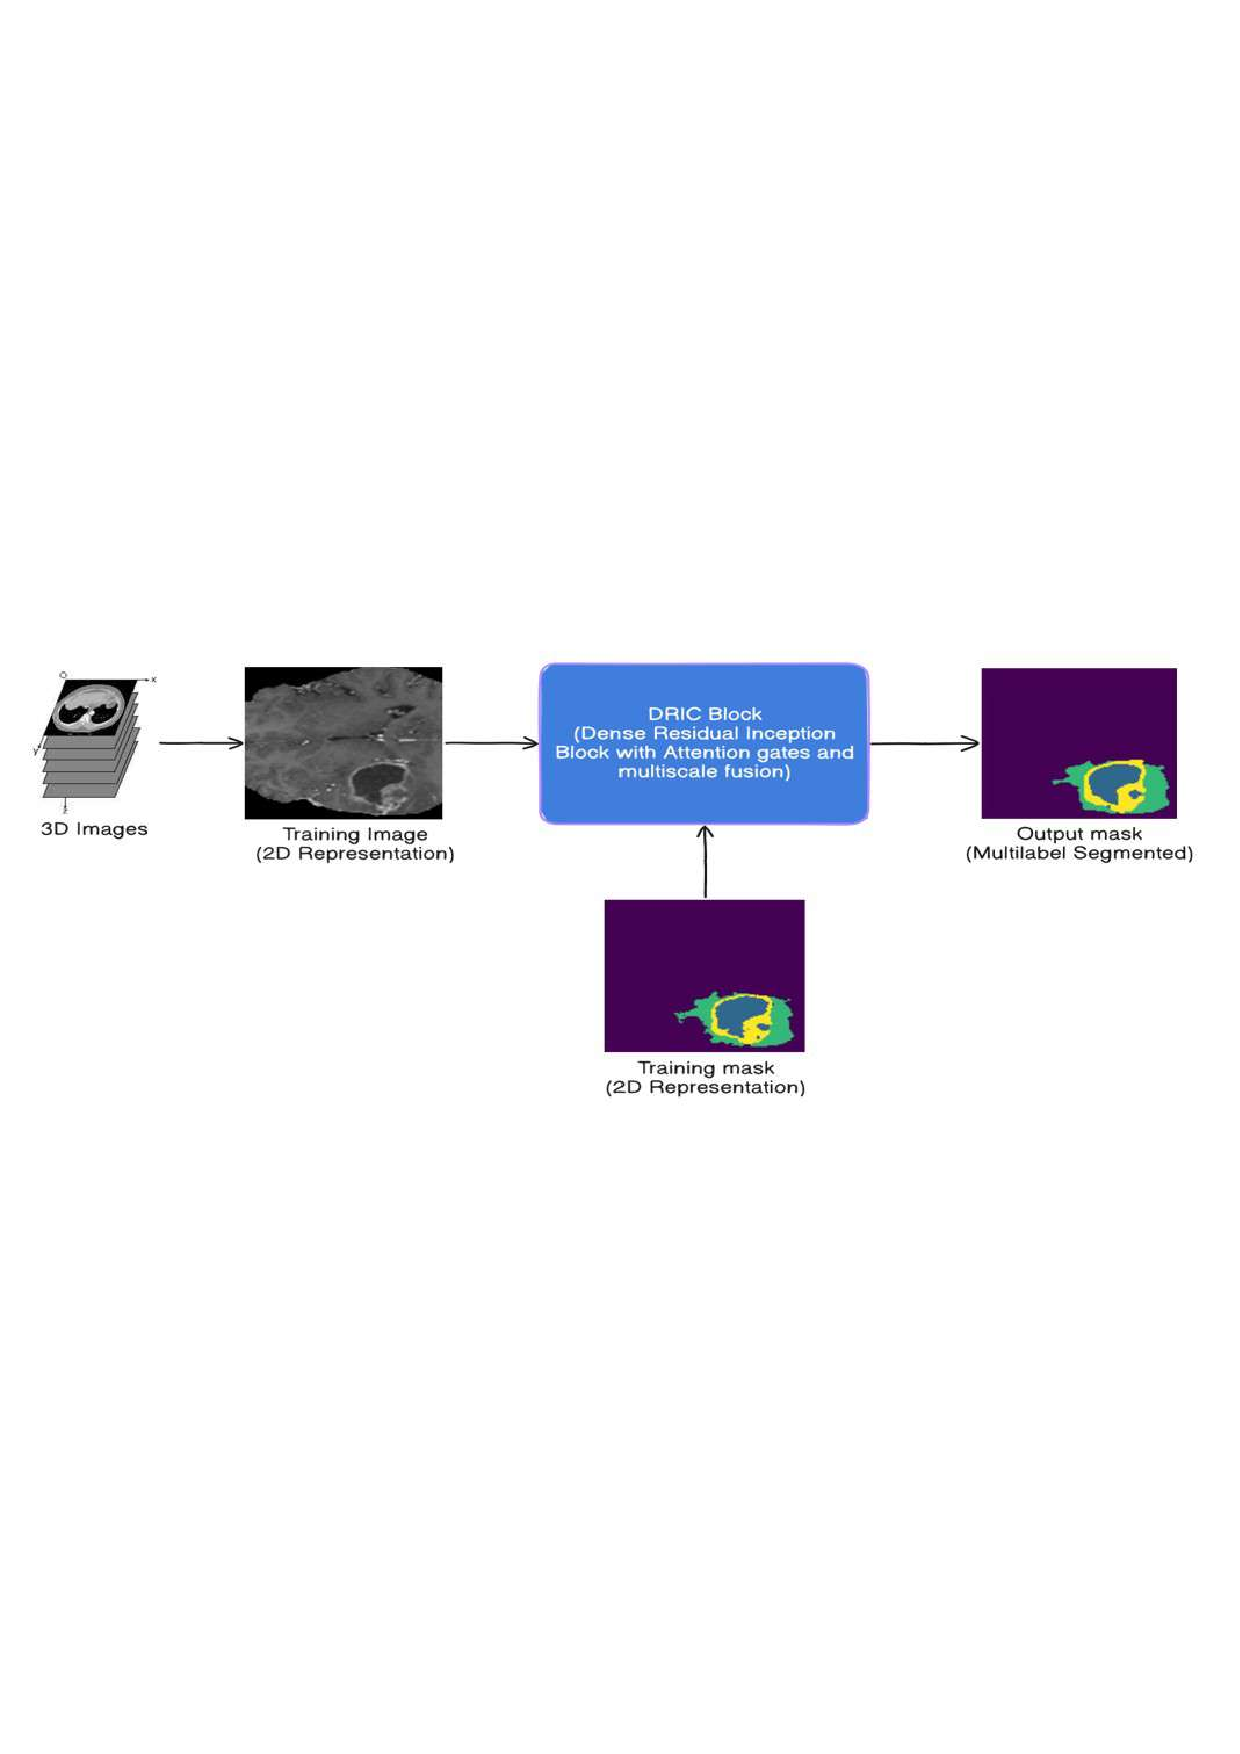
\includegraphics{figs/Graphical Abstract.pdf}
%\end{graphicalabstract}

% Research highlights
\begin{highlights}
    \item Research highlights item 1
    \item Research highlights item 2
    \item Research highlights item 3
\end{highlights}

% Keywords — each keyword separated by \sep
\begin{keywords}
Dense Residual Inception Convolution (DRIC) blocks \sep
Attention gates \sep
Multiscale feature fusion module \sep
U-Net \sep
Adaptive hybrid loss function
\end{keywords}


\maketitle

\begin{figure*}[!htb]
    \centering
    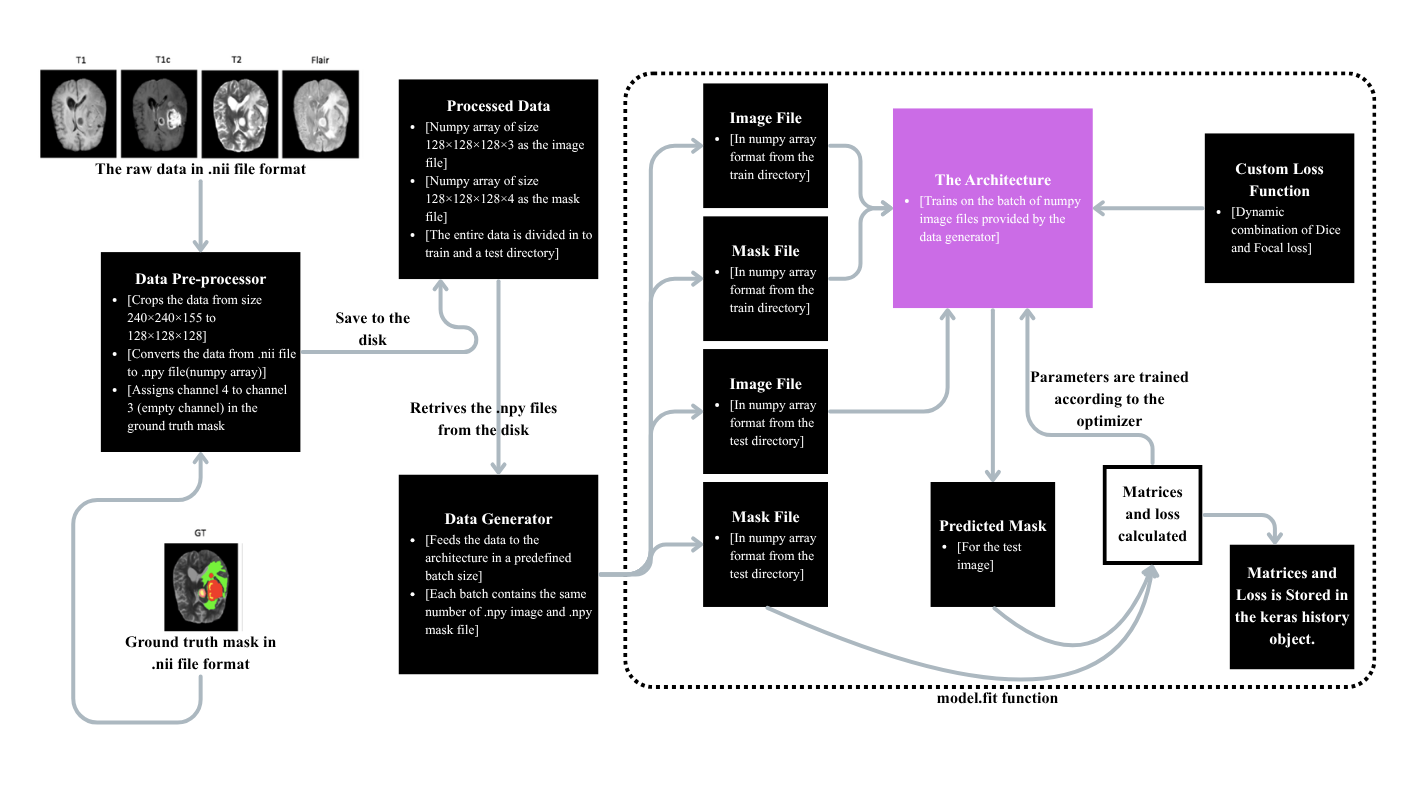
\includegraphics[width=\textwidth]{figs/Abstract Graphical.png}
    \caption{Graphical illustration of the proposed framework.}
    \label{fig:graphical_abstract}
\end{figure*}


%% ============================================================
%% SECTION: Introduction
%% ============================================================

\section{Introduction}

Brain tumor \cite{deangelis2001brain} encompasses various abnormal growths called neoplasms with distinct biology, prognosis, and treatment, often referred to as intracranial neoplasms. Modern medical science has advanced significantly in the understanding of the human brain, now using technologies like Magnetic Resonance Imaging (MRI) \cite{hashemi2012mri,brown2011mri} for non-invasive visualization and diagnosis of life-threatening diseases such as brain tumors. Magnetic Resonance Imaging (MRI) is a highly promising imaging modality that provides multicontrast information and fine anatomical detail for accurate tumor segmentation and precise boundary delineation, while also supporting tumor growth prediction, early prognosis, treatment optimization, and improved evaluation of patient outcomes \cite{amin2020distinctive}. Despite the advantages of MRI, brain tumor segmentation remains an inherently complex and challenging task due to the complex nature of certain tumor types, such as gliomas and glioblastomas. Gliomas and glioblastomas \cite{bahadure2017image} are difficult to accurately segment due to their diffuse boundaries, irregular shapes, and poor contrast with surrounding tissue, along with the wide variability in their appearance in different regions of the brain and imaging protocols. In addition to that, Glioblastomas exhibit infiltrative growth, which makes their margins indistinct from normal tissue. To improve delineation, multiple MRI modalities such as T1, T1 contrast enhanced (T1ce), T2, PD, dMRI, and fluid attenuated inversion recovery (FLAIR) are utilized, as complementary contrasts provide quasi-unique tissue signatures \cite{li2019multi, islam2021glioblastoma, rathore2018radiomic, hasan2016segmentation}.

The lack of standardization in the intensities of the MRI voxels further complicates the segmentation, as identical tumor tissues can present differently depending on the strength of the scanner and the acquisition settings. Consequently, automated annotation of volumetric MRI images has become an essential deep learning endeavor in supporting healthcare professionals to simplify and unify the process of labeling intricate 3D medical images for precise and consistent analysis. Conventional automatic brain tumor segmentation techniques rely predominantly on handcrafted feature engineering \cite{menze2014multimodal}, following a traditional machine learning framework where feature extraction and classifier training are performed independently. In contrast, deep neural networks enable end-to-end learning of hierarchical, task-specific feature representations directly from multimodal MRI data, facilitating more effective brain tumor segmentation \cite{bengio2013representation}.

Accurate and efficient brain tumor segmentation from multimodal MRI remains a challenge due to the substantial variability in tumor appearance, size, location, and morphology. Mohammad Havaei et al.~\cite{havaei2017brain} proposed a fully automatic deep convolutional neural network framework that integrates local and global contextual features, class-imbalance-aware training, and cascaded refinement to achieve competitive BraTS segmentation performance with reduced computational complexity and inference time. El-Sayed A et al.~\cite{el2014computer} proposed a hybrid machine learning framework that combines pulse-coupled neural network-based segmentation, wavelet feature extraction, principal component analysis, and neural network classification, achieving high accuracy in distinguishing normal and abnormal brain MRI scans while demonstrating robustness and computational efficiency. In addition, their comprehensive review of contemporary CAD-based brain MRI segmentation and classification techniques \cite{maitra2008hybrid, el2010hybrid, cheng2010automated, cherkassky2007learning} provided valuable insights into existing challenges and future research directions.

Despite the promising results reported by existing CAD systems and deep learning-based approaches, accurate segmentation of heterogeneous brain tumor subregions from volumetric MRI data remains a challenging problem. The limitations of handcrafted feature-based methods and the growing demand for exploiting three-dimensional spatial context have encouraged the development of 3D MRI segmentation frameworks capable of learning more discriminative tumor representations. Motivated by these observations, this work proposes a novel 3D deep learning-based brain tumor segmentation framework to improve segmentation accuracy and robustness while maintaining computational efficiency.

\vspace*{-1\baselineskip}


%% ============================================================
%% SECTION: Related Work
%% ============================================================

\section{Related work}

\subsection{Motivation}

Brain MRI data are inherently volumetric, which makes the exploitation of three-dimensional spatial information crucial for accurate tumor delineation. Consequently, 3D convolutional neural networks have emerged as a promising paradigm for brain tumor segmentation, as they can effectively model inter-slice contextual relationships and complex tumor morphology. Recent studies have demonstrated the potential of 3D deep learning architectures for improving segmentation performance on benchmark datasets such as BraTS ~\cite{abidin2024recent,krishnapriya2023survey,zhang2024etunet}. [To add more related works under this section, followed by Proposed Framework] Inspired by these developments, the present work explores a 3D deep learning framework for robust and computationally efficient brain tumor segmentation.

\subsection{Contribution}


%% ============================================================
%% SECTION: Our Proposal
%% ============================================================

\section{Our Proposal}

In this work, we adopt a Three-Dimensional Convolutional Neural Network (3D-CNN) framework tailored for the segmentation of volumetric brain tumors. Unlike Two-Dimensional slice-based methods, our model operates directly on cropped volumes of size $128\times128\times128$, thus preserving the spatial context across all three dimensions. The network input consists of three MRI modalities: T1 contrast enhanced (T1ce), T2 and FLAIR stacked as channels, while the T1 modality is excluded to avoid redundancy, as T1ce provides most of the anatomical information available in T1 while additionally highlighting contrast-enhanced regions. Our Convolutional approach is built on the classical U-Net shape backbone where there is an encoder (contracting path) and a decoder (expanding path) connected through a bottleneck and skip connections(residual connections). But in our approach we replace the classical $3\times3\times3$ convolution used for the basic U-net with custom Dense Inception Residual Convolution (DRIC) blocks to capture multi-scale features and attention gates to selectively emphasize tumor regions during feature propagation through skip connections. Although computationally more demanding, 3D convolutions were adopted to preserve volumetric context rather than segmenting each 2D slice as in our literature review, which tends to capture more volumetric context. To address the high memory requirements of 3D volumetric images by cropping into the data and discarding the empty spaces present. Now, there are few major components that make up our approach in building this architecture.


%% ============================================================
%% SECTION*: Part I — Module-Wise Architectural Description
%% ============================================================

\section*{Part I: Module-Wise Architectural Description}

\subsection{Dense Inception Residual Convolution (DRIC) Blocks}

The first step in improving the classical U-Net architecture is to replace the $3\times3\times3$ convolution with something more modern that can capture both fine and coarse features in a single go. To address this limitation, inception-style parallel convolutions are employed, where parallel convolutional operations are performed using multiple sizes of kernels to extract feature on every scale. In our approach, we also added Dense and Residual Connections in the block so that feature preservation is improved during deep feature transformation. So, the fundamental feature extraction unit in our architecture combines three design principles: inception-style multi-branch convolution, dense connectivity, and residual learning, shown in Figure \ref{FIG:DRIC Block}.

\begin{center}
\begin{minipage}{\columnwidth}
    \centering

    % Main Figure
    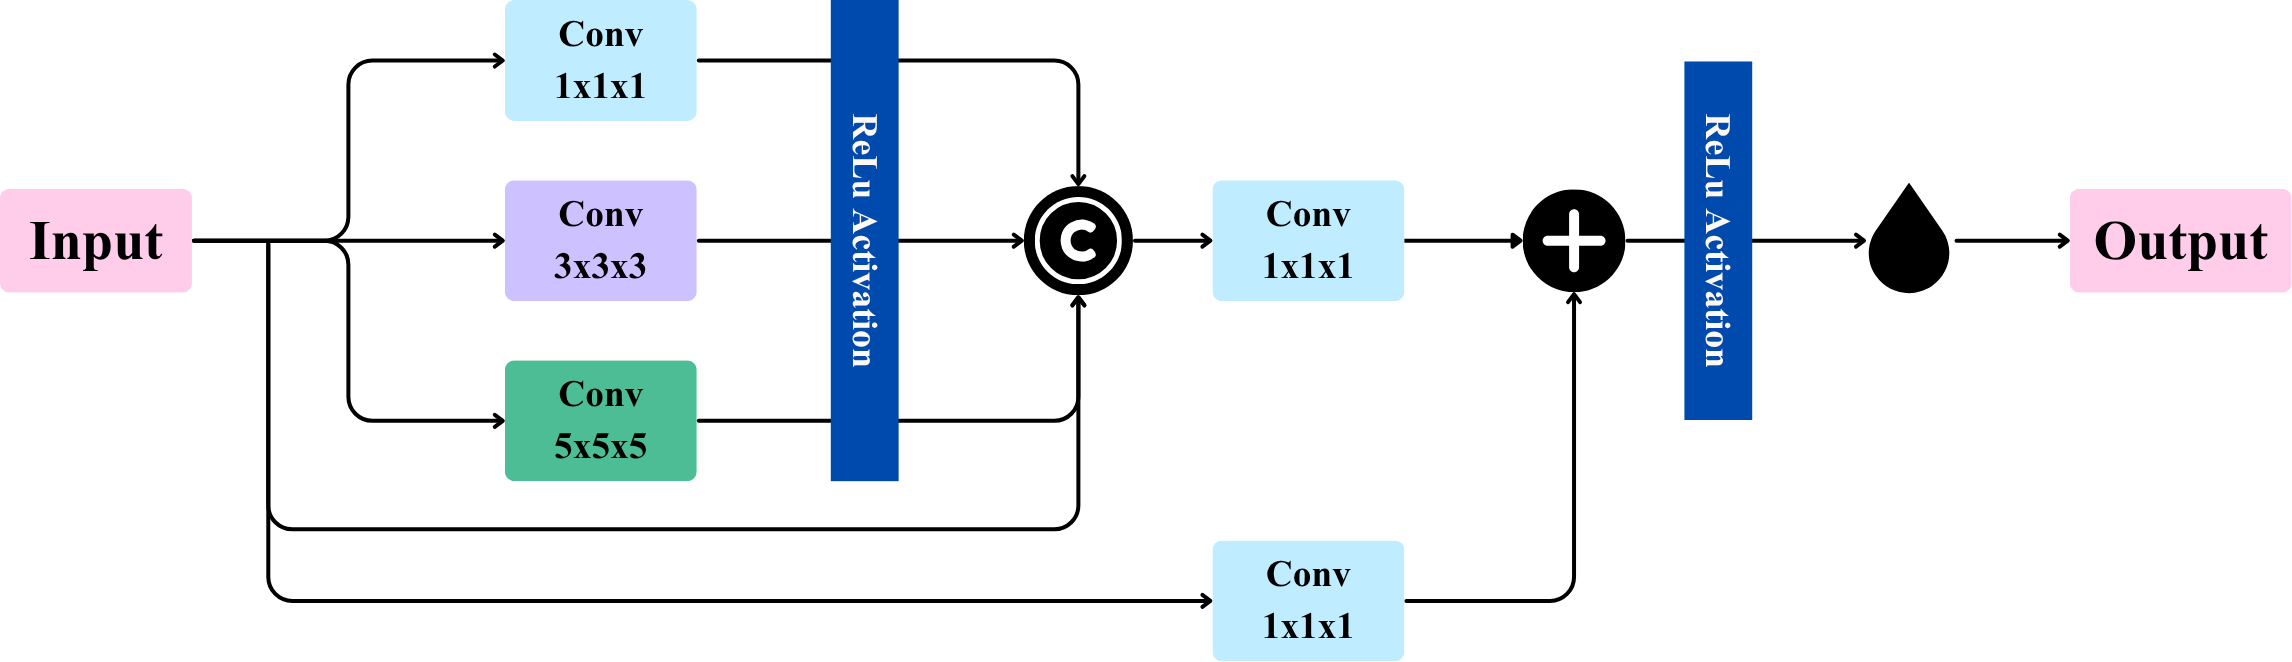
\includegraphics[
        height=0.085\textheight,
        width=0.9\textwidth
    ]{figs/Dense Inception-Residual Block.png}

    \vspace{1mm}

    % Dashed line settings
    \setlength{\dashlinedash}{0.5pt}
    \setlength{\dashlinegap}{1.5pt}

    % Legend Box
    \fbox{
    \begin{tabular}{cl|cl|cl}
        
\includegraphics[width=0.018\textwidth]{figs/Label1/1.png}
        & \hspace{-1.3em}\scriptsize Concatenation
        &
        
\includegraphics[width=0.018\textwidth]{figs/Label1/6.png}
        & \hspace{-1.3em}\scriptsize Dropout
        &
        
\includegraphics[width=0.018\textwidth]{figs/Label1/5.png}
        & \hspace{-1.3em}\scriptsize Add
    \end{tabular}
    }

    \captionof{figure}{Dense Inception-Residual Block}
    \label{FIG:DRIC Block}
\end{minipage}
\end{center}

\subsubsection{Inception-style multi-branch convolution}

Traditional convolutional layers use a single kernel size, which limits the receptive field per layer. Instead, the DRIC block applies multiple convolutional kernels of different sizes in parallel to capture features at different spatial scales. Formally, let the input tensor for the block be: $X\in H \times W \times D \times C_{in}$, where $H, W, D$ denote spatial dimensions, and $C_{in}$ is the number of input channels. Each branch applies a convolution with kernel size $\kappa\in 1,3,5:$
$F_k = \sigma(\mathcal W_k * X + b_k ), k\in 1,3,5,$ where * denotes 3D convolution, $\mathcal W_k$ and $b_k$ are trainable weights and biases, and $\sigma(\cdot)$ is a non-linear activation function (ReLU in our implementation).
The multi-branch outputs are concatenated channel-wise: $F_{concat} =[F_1 \| F_3 \| F_5 ],$ yielding a feature tensor enriched with both local fine details ($1\times 1\times 1$ and $3\times 3\times 3$) and broader contextual information ($5\times 5\times 5$).

\subsubsection{Dense connectivity}

To encourage feature reuse and strengthen gradient flow, the DRIC block incorporates dense connections. Instead of passing only the output of the previous block, the concatenation includes the input feature maps: $F_{dense} =[X \| F_{concat}]$. This ensures that each layer has direct access to all preceding feature maps, reducing redundancy, and improving parameter efficiency.

\subsubsection{Residual learning}

Direct stacking of inception-dense modules may increase feature dimensionality excessively, leading to optimization difficulties. To address this, the DRIC block applies a residual connection to stabilize training. A $1\times 1\times 1$ convolution is used to match the dimensions between the input and output before addition: $F_{res} =\sigma (\mathcal W_{res} * X + b_{res})$. Finally, the output of the DRIC block is: $Y = F_{dense} +F_{res}$. This residual formulation mitigates vanishing gradients and accelerates convergence by allowing the block to learn perturbations over the identity mapping rather than the full transformation.

\subsection{Multi-Scale Input Strategy}

\begin{center}
    \centering

    % Main Figure
    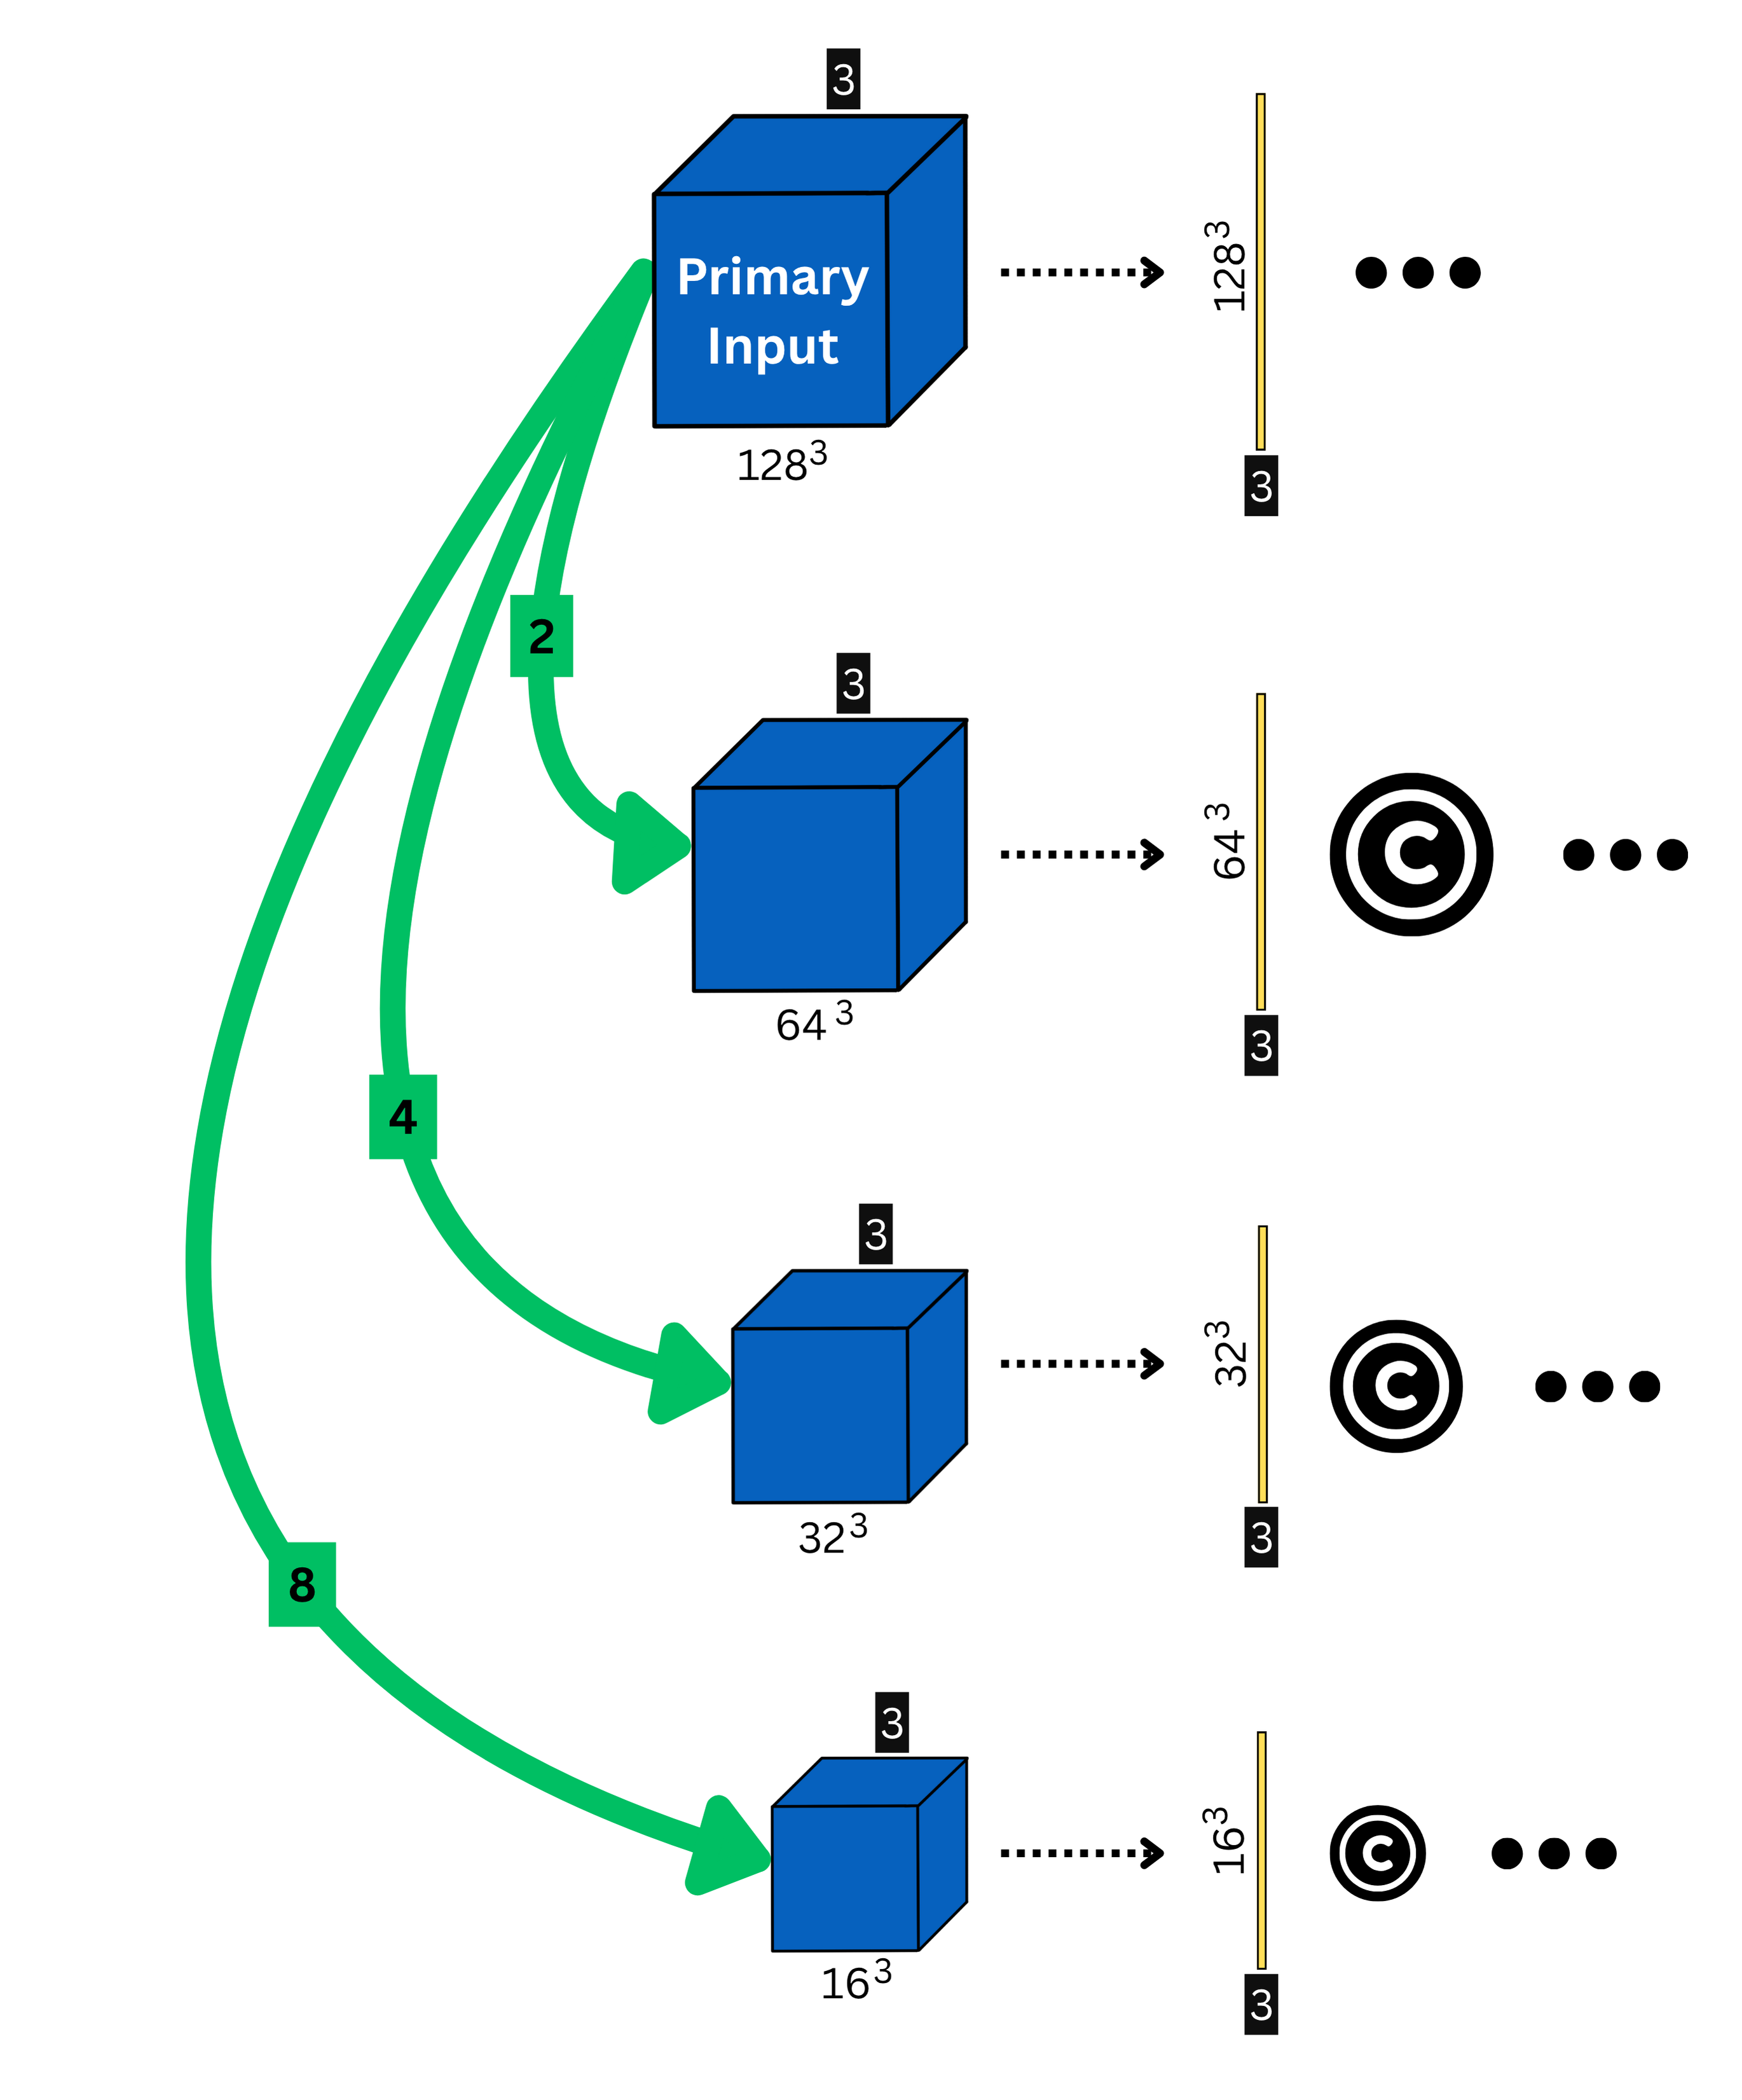
\includegraphics[
        %height=0.22\textheight,
        width=0.3\textwidth
    ]{figs/Input, Multi-Scale Paths.png}

    \vspace{2mm}

    % Dashed line settings
    \setlength{\dashlinedash}{0.5pt}
    \setlength{\dashlinegap}{1.5pt}

    % Legend Box
    \fbox{
    \begin{tabular}{cl|cl}
        
\includegraphics[width=0.018\textwidth]{figs/Label1/1.png}
        & \scriptsize Concatenation
        &
        
\includegraphics[width=0.032\textwidth]{figs/Label1/2.png}
        & \scriptsize Average-pooled by factor of $n$
        \\[1.5mm]
        \hdashline
        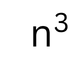
\includegraphics[width=0.030\textwidth]{figs/Label1/3.png}
        & \scriptsize Dimension
        &
        
\includegraphics[width=0.030\textwidth]{figs/Label1/4.png}
        & \scriptsize Number of channels
    \end{tabular}
    }

    \captionof{figure}{Multi-Scale Input Strategy}
    \label{FIG:Multi-Scale Input}
\end{center}

To enhance contextual understanding of tumors with highly variable size and appearance, our network incorporates a multi-scale input strategy shown in Figure \ref{FIG:Multi-Scale Input}. Instead of relying only on the hierarchical down-sampling of the encoder, we explicitly inject down-sampled versions of the input volume into the corresponding encoder stages.
Let the input be $X_0\in \mathbb{R}^{(128\times 128\times 128\times C)}, C=3,$ where $C$ is the number of MRI modalities (T1ce, T2, FLAIR). Scaled versions are obtained by applying a down-sampling operator $S_\kappa (\cdot): X_0^{(i)}=S_{2^{(i-1)}}(X_0), i=1,\cdots, 4,$ producing inputs at resolutions $128^3, 64^3, 32^3,$ and $16^3$. Each $X_0^{(i)}$ is passed through a shallow convolutional stem to produce features $F_0^{(i)},$ that are concatenated with encoder features $F_{l} $ at the corresponding stage $Z_{l} =Concat(F_{l} ,F_0^{(i)})$.
This design ensures that fine-scale structures ($e_\cdot g_\cdot$ enhancing tumor cores) are reinforced by high-resolution features, while large-scale abnormalities ($e_\cdot g_\cdot$ edema) benefit from the coarse global context. Empirically, the multi-scale input improved boundary precision and reduced false positives compared to encoder-only baselines.


\subsection{Encoder (Contracting Path)}

\begin{center}
    \centering

    % Main Figure
    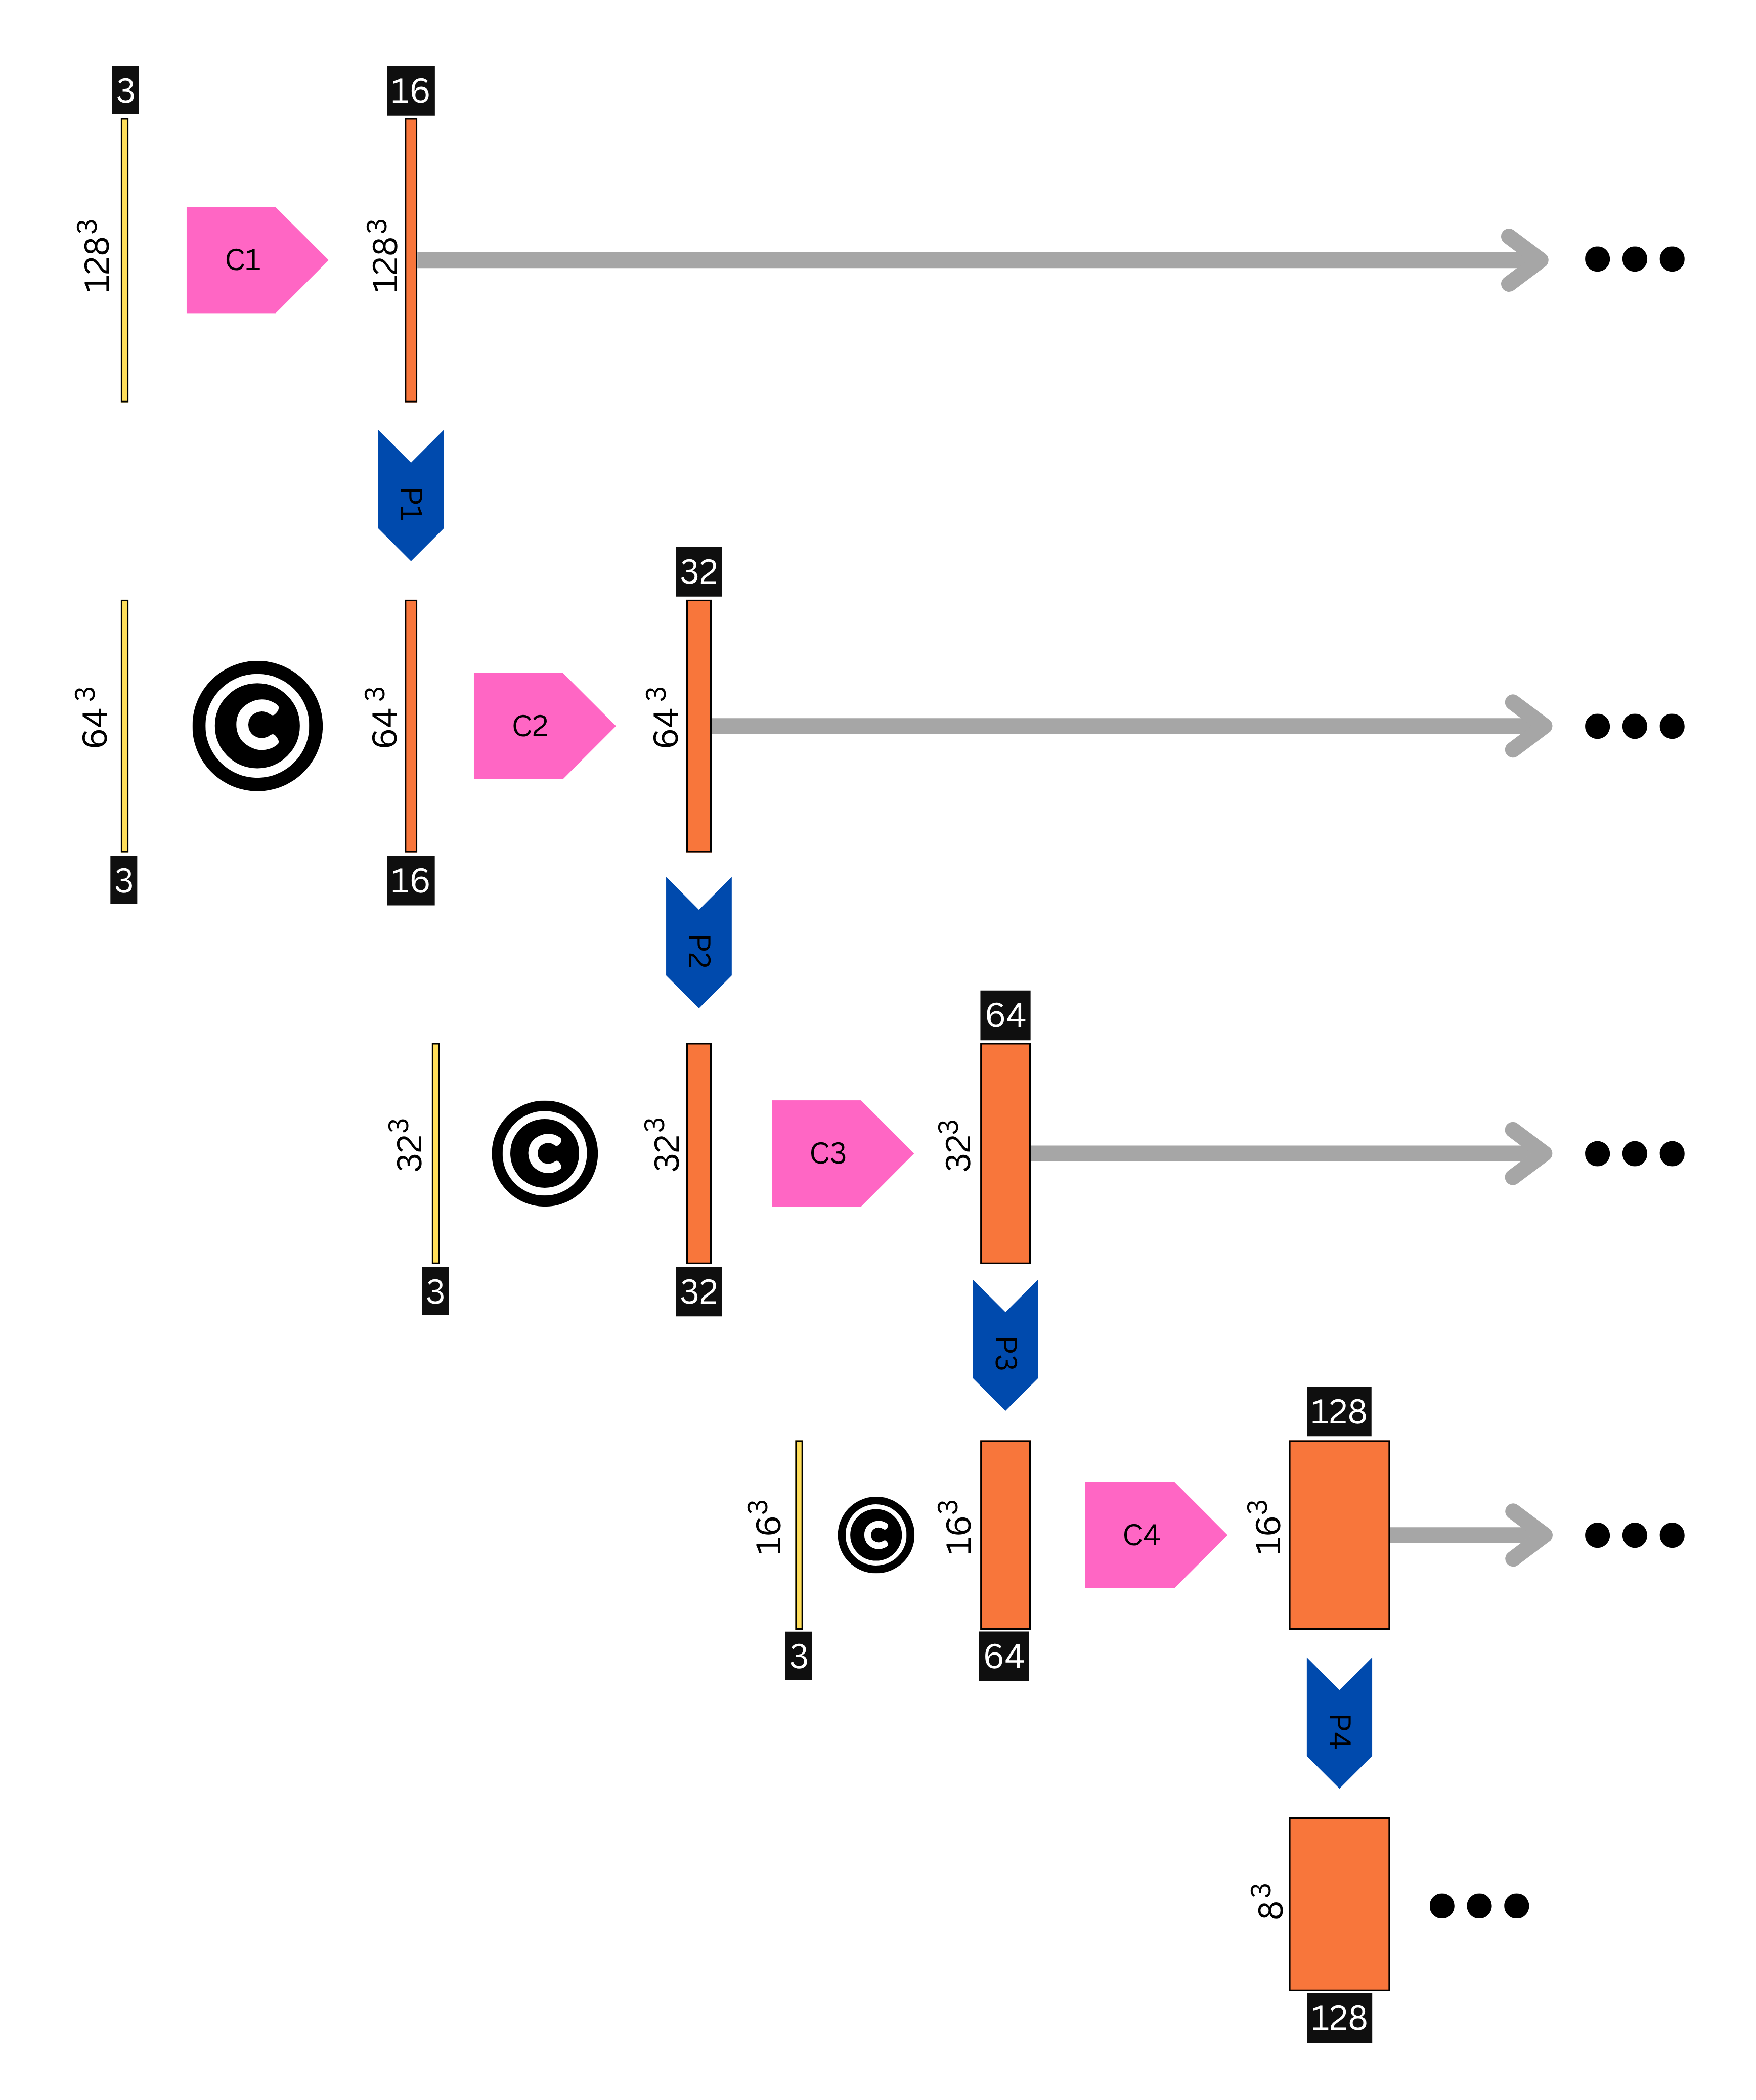
\includegraphics[
        %height=0.22\textheight,
        width=0.3\textwidth
    ]{figs/Encoder Path.png}

    \vspace{2mm}

    % Dashed line settings
    \setlength{\dashlinedash}{0.5pt}
    \setlength{\dashlinegap}{1.5pt}

    % Legend Box
    \fbox{
    \begin{tabular}{cl|cl}
        
\includegraphics[width=0.018\textwidth]{figs/Label1/1.png}
        & \scriptsize Concatenation
        &
        
\includegraphics[width=0.015\textwidth]{figs/Label1/9.png}
        & \scriptsize MaxPool
        \\[1.5mm]
        \hdashline
        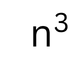
\includegraphics[width=0.030\textwidth]{figs/Label1/3.png}
        & \scriptsize Dimension
        &
        
\includegraphics[width=0.030\textwidth]{figs/Label1/4.png}
        & \scriptsize Number of channels
        \\[1.5mm]
        \hdashline
        
\includegraphics[width=0.030\textwidth]{figs/Label1/8.png}
        & \scriptsize Dense Inception-Res Block
    \end{tabular}
    }

    \captionof{figure}{Encoder Path}
    \label{FIG:Contracting Path}
\end{center}

The encoder path, in Figure \ref{FIG:Contracting Path}, of our network is designed to progressively down-sample the input volume while simultaneously extracting rich hierarchical features. This is achieved by stacking multiple DRIC blocks interleaved with down-sampling operations (3D max-pooling).
Let the network input be: $X\in \mathbb{R}^{(H\times W\times D\times C_0)},$ where in our implementation the spatial dimensions are $128\times 128\times 128$ with $C_0 = 3$ representing the number of input channels, namely T1ce, T2 and FLAIR. Applying a DRIC block to each encoder stage $l$, the transformation corresponds to: $F_l=DRIC_l(X_{l-1}),$ where $X_{l-1}$ is the input to stage $l$, and $F_l$ is the output feature tensor. Extending the prior definition of the DRIC block $F_l$ can be expressed as $F_l=[X_{l-1} \| \sigma(W_1 *X_{l-1}) \| \sigma(W_3 *X_{l-1} ) \| \sigma(W_5 *X_{l-1} )]+W_{res} *X_{l-1}$, where $1, 3,$ and $5$ represent the kernel sizes in the inception-style parallel branches, while the final summation corresponds to the residual mapping.
After feature extraction, spatial resolution is reduced by applying 3D max pooling with stride 2:   $X_l=MaxPool3D(F_{l,p=2}),$ where $p$ is the size of pooling window. This leads to a twofold reduction in spatial dimensions: $H_l=\tfrac{H_{l-1}}{2}, W_l=\tfrac{W_{l-1}}{2}, D_l=\tfrac{D_{l-1}}{2}$. Thus, the encoder creates progressively deeper representations while shrinking the spatial extent.
The encoder is composed of L-stages, each consisting of one DRIC block followed by down-sampling. In practice, $L=4$. The recursive formulation is: $X_l=MaxPool3D(DRIC_l (X_{l-1})), l=1,\cdots,L$.
At the end of the encoder, we obtain a multi-resolution feature pyramid: $F=\{F_1,F_2,\cdots,F_L\},$ where $F_l$ represents features at stage $l$ before pooling. These tensors are later forwarded to the decoder through skip connections.


\subsection{Decoder (Expanding Path)}

\begin{center}
    \centering

    % Main Figure
    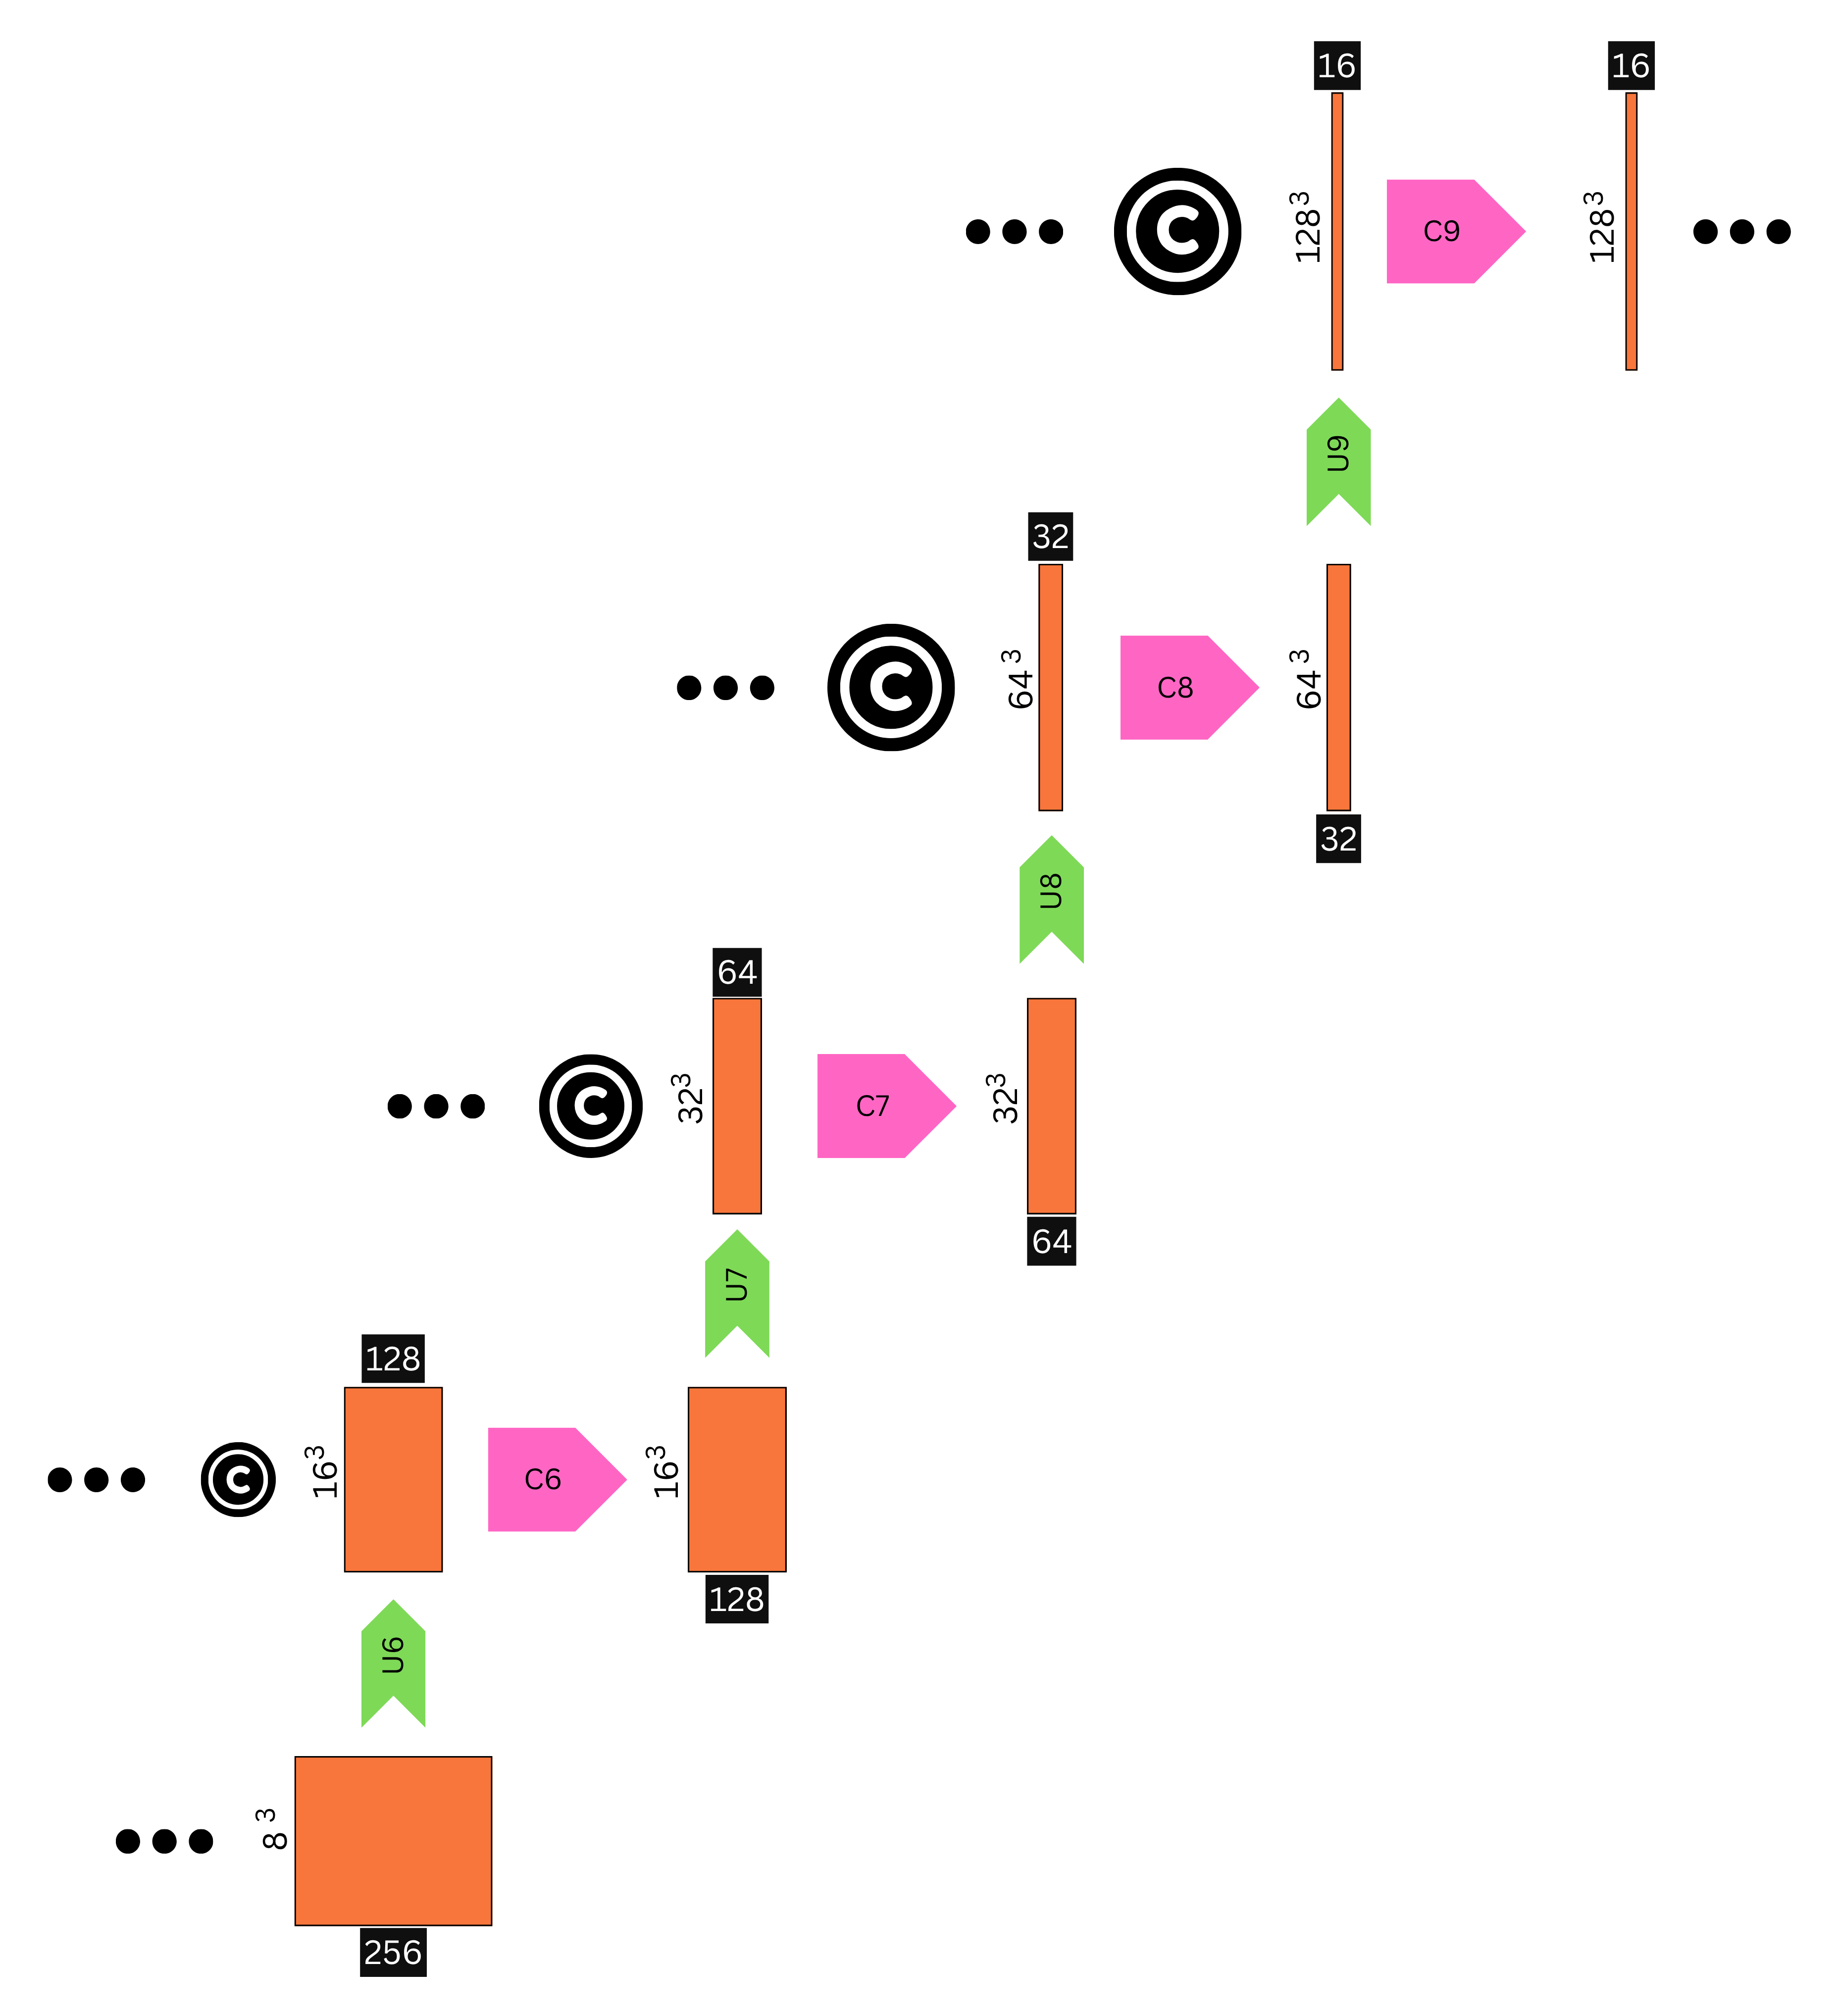
\includegraphics[
        height=0.22\textheight,
        width=0.33\textwidth
    ]{figs/Decoder Path.png}

    \vspace{2mm}

    % Dashed line settings
    \setlength{\dashlinedash}{0.5pt}
    \setlength{\dashlinegap}{1.5pt}

    % Legend Box
    \fbox{
    \begin{tabular}{cl|cl}
        
\includegraphics[width=0.018\textwidth]{figs/Label1/1.png}
        & \scriptsize Concatenation
        &
        
\includegraphics[width=0.015\textwidth]{figs/Label1/7.png}
        & \scriptsize TransConv
        \\[1.5mm]
        \hdashline
        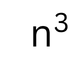
\includegraphics[width=0.030\textwidth]{figs/Label1/3.png}
        & \scriptsize Dimension
        &
        
\includegraphics[width=0.030\textwidth]{figs/Label1/4.png}
        & \scriptsize Number of channels
        \\[1.5mm]
        \hdashline
        
\includegraphics[width=0.030\textwidth]{figs/Label1/8.png}
        & \scriptsize Dense Inception-Res Block
    \end{tabular}
    }

    \captionof{figure}{Decoder Path}
    \label{FIG:Expanding Path}
\end{center}

The decoder path, in Figure \ref{FIG:Expanding Path}, of our network is designed to progressively up-sample the compressed bottleneck representation and reconstruct the segmentation mask at full resolution. This is achieved by combining learned up sampling operators, attention-gated skip connections, and DRIC blocks for feature refinement.
Let the bottleneck feature map be: $X\in \mathbb{R}^{(H_B\times W_B\times D_B\times C_B)}, where H_B, W_B, D_B$ are the spatial dimensions of the bottleneck and $C_B$ the number of channels. The decoder consists of $L$ stages that mirror the depth of the encoder.
At each decoder stage $l$, the first operation is learned up-sampling by a 3D transposed convolution: $U_l=ConvTranspose3D(X_{l+1},k=2,s=2),$ where $k$ is the kernel size and s the stride. This doubles the spatial dimensions: $H_l=2H_{l-1}, W_l=2W_{l-1}, D_l=2D_{l-1}$.
The up sampled tensor $U_l$ is then fused with the encoder feature map $F_l$ via an attention gate. The gating function suppresses irrelevant encoder activations and is defined as: $S_l=\alpha_l\odot F_l, \alpha_l=\sigma(W_u U_l+W_e F_l+b),$ where $\sigma$ is the sigmoid function, $W_u, W_e$ are learnable projections and $\odot $ is element-wise multiplication. This ensures that only the salient encoder features are propagated.
The decoder feature at stage $l$ is then formed by concatenating the up-sampled tensor and the attended skip features: $C_l= U_l \| S_l$ followed by calling the DRIC block to integrate multi-scale convolutions and residual mappings as $F_l^{'}= DRIC_l (C_l)$.
The recursive formulation of the decoder is thus: {\small$X_l= DRIC_l (Concat(ConvTranspose3D(X_{l+1}),A(F_l,X_{l+1})))$}; where $l = L,\cdots,1$, and $A(\cdot)$ denotes the attention gate.
At the final stage, the reconstructed feature map has the same resolution as the input volume. A $1\times 1\times 1$ convolution followed by a voxel-wise softmax projects it to class probabilities: $\hat{Y} = Softmax(W_0 * X_1 + b_0), \hat{Y} \in \mathbb{R}^{H\times W\times D\times K},$ where $K$ is the number of segmentation classes. Each voxel $(i,j,k)$ is assigned a label by: $\hat{y}_{(i,j,k)} = \arg\max \hat{Y}^{(c)}_{(i,j,k)}$.
Thus, the decoder path progressively restores spatial detail while leveraging both encoder information (via attention-gated skip connections) and multi-scale feature extraction (via DRIC refinement).


\subsection{Skip Connections, Attention Gates and Bottlenecks}

\begin{center}
    \centering
    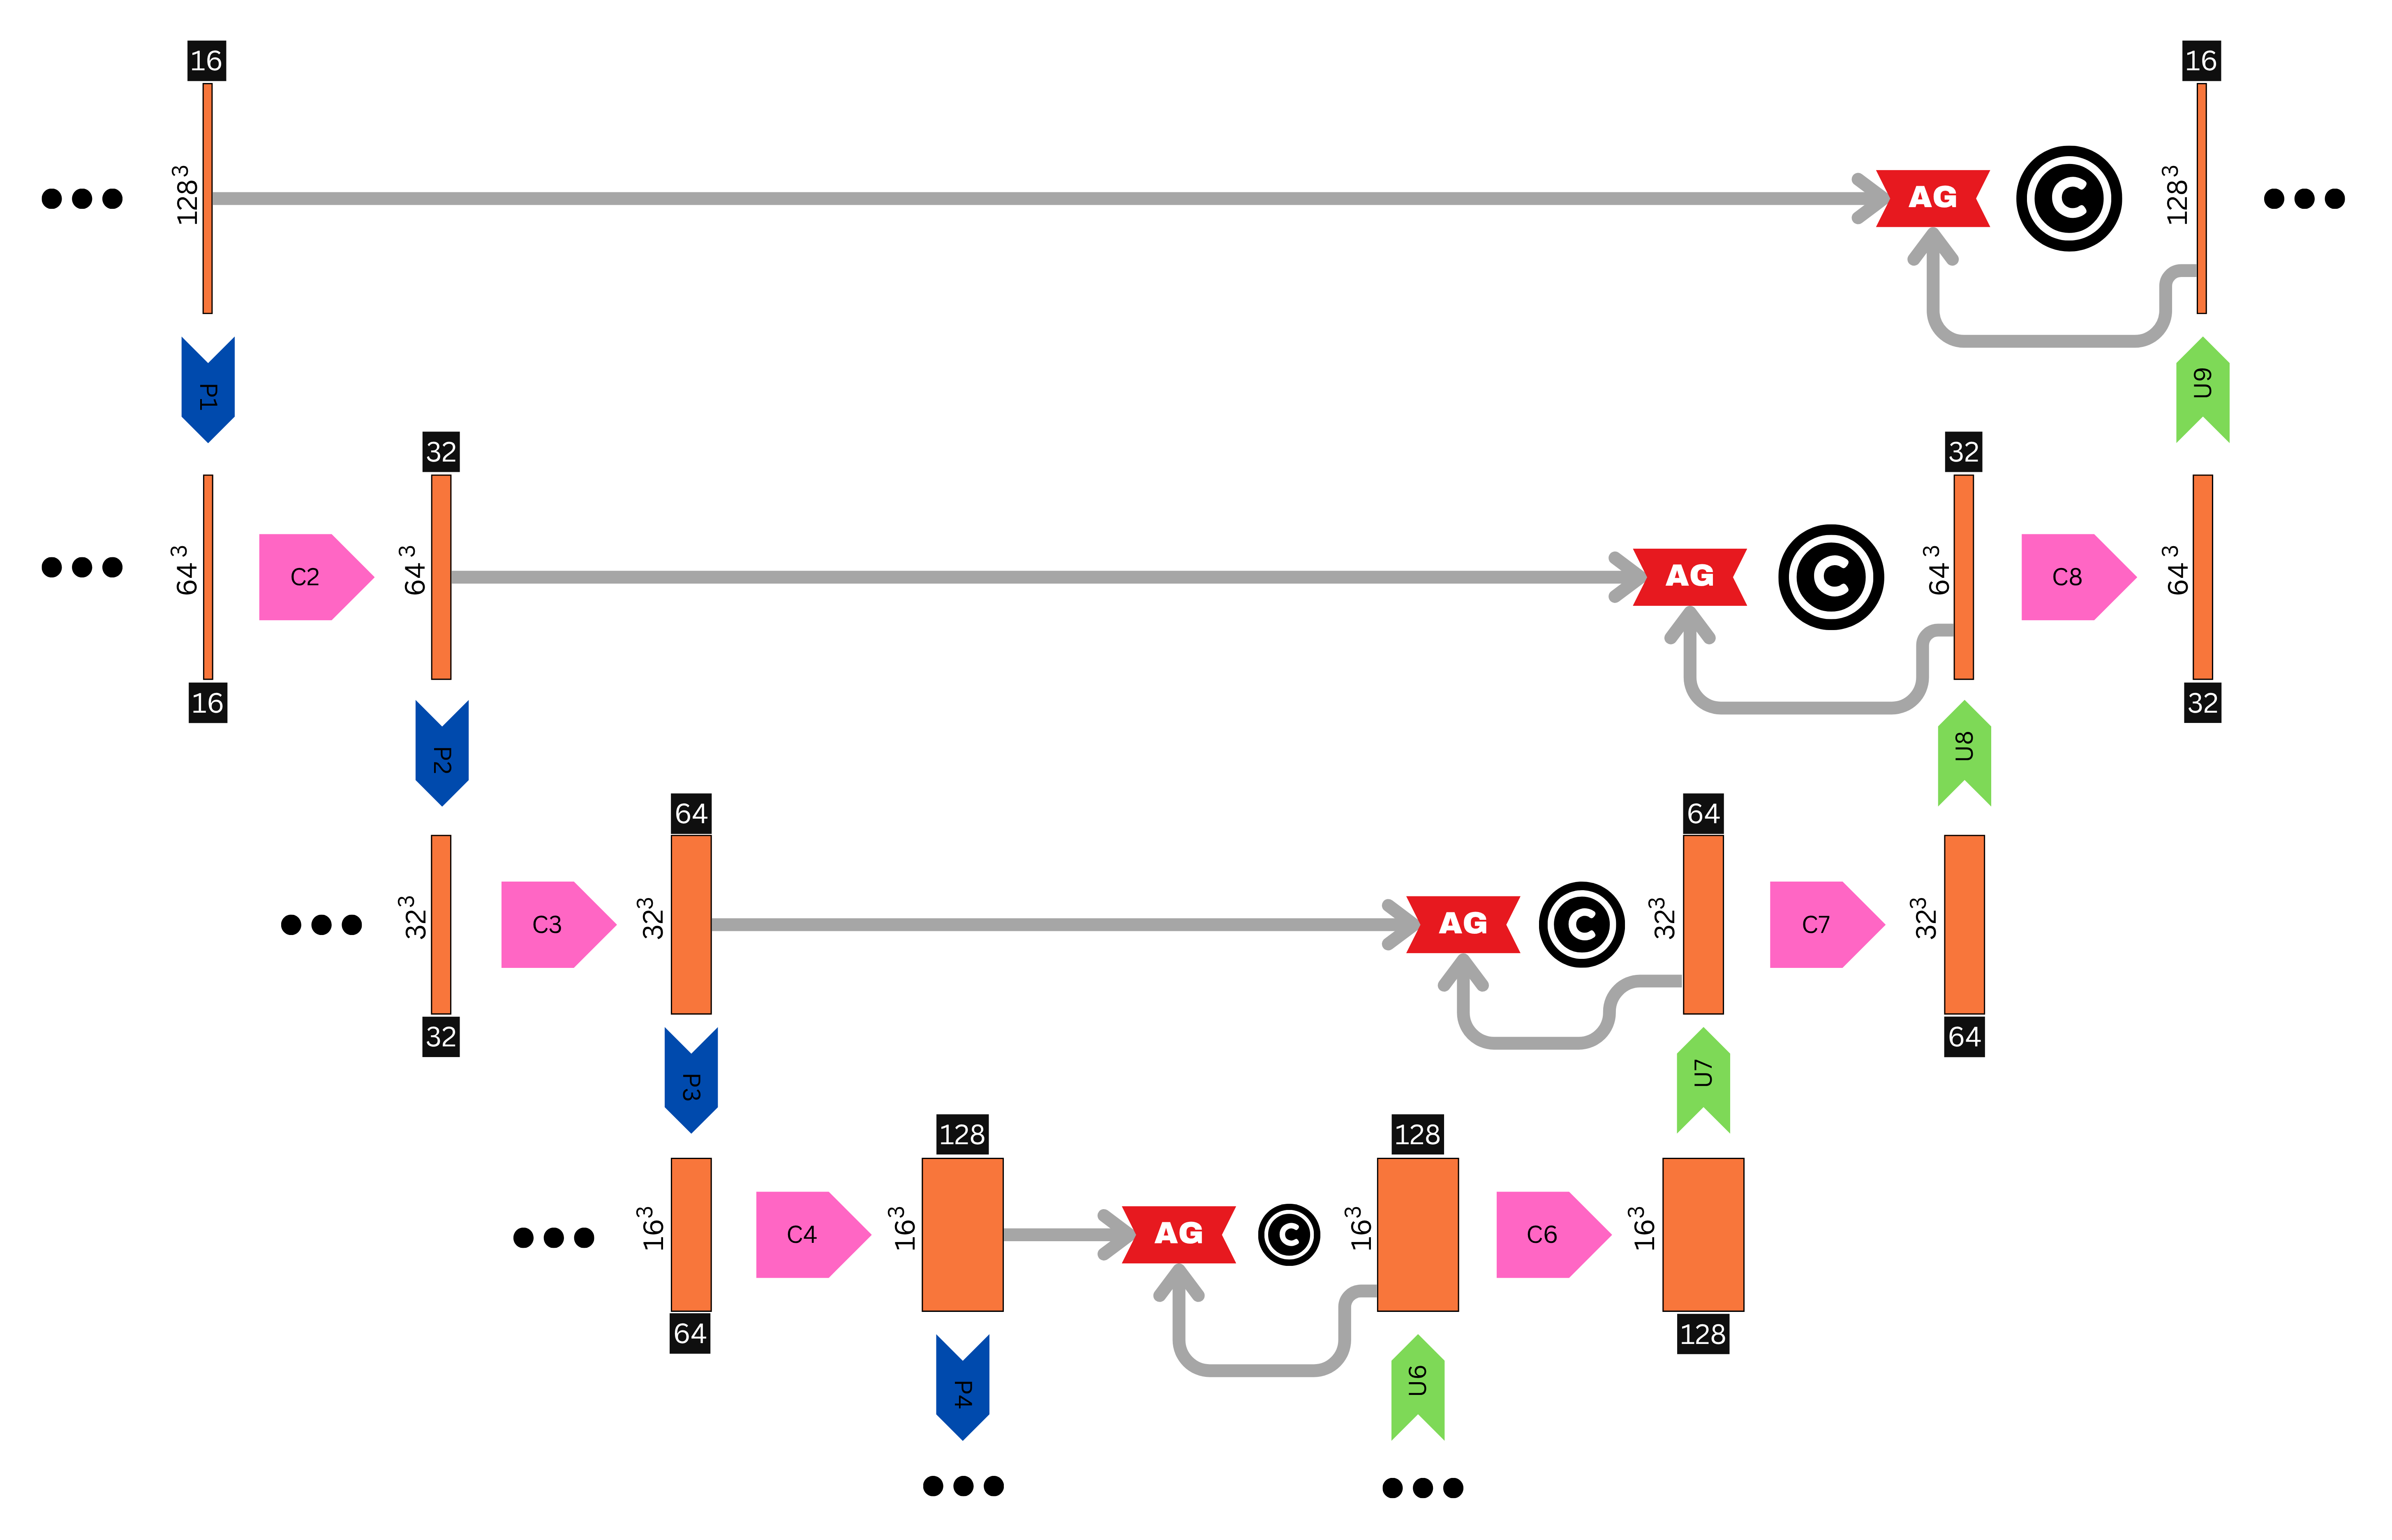
\includegraphics[height=0.17\textheight, width=0.4\textwidth]{figs/Attention gates over skip connections.png}

    \vspace{2mm}

    % Dashed line settings
    \setlength{\dashlinedash}{0.5pt}
    \setlength{\dashlinegap}{1.5pt}

    % Legend Box
    \fbox{
    \begin{tabular}{cl|cl}
        
\includegraphics[width=0.018\textwidth]{figs/Label1/1.png}
        & \scriptsize Concatenation
        &
        
\includegraphics[width=0.015\textwidth]{figs/Label1/9.png}
        & \scriptsize MaxPool
        \\[1.5mm]
        \hdashline
        
\includegraphics[width=0.015\textwidth]{figs/Label1/7.png}
        & \scriptsize TransConv
        &
        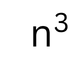
\includegraphics[width=0.030\textwidth]{figs/Label1/3.png}
        & \scriptsize Dimension
        \\[1.5mm]
        \hdashline
        
\includegraphics[width=0.030\textwidth]{figs/Label1/4.png}
        & \scriptsize Number of channels
        &
        
\includegraphics[width=0.030\textwidth]{figs/Label1/8.png}
        & \scriptsize Dense Inception-Res Block
        \\[1.5mm]
        \hdashline
        
\includegraphics[width=0.030\textwidth]{figs/Label1/10.png}
        & \scriptsize AttentionGate
    \end{tabular}
    }

    \captionof{figure}{Skip Connections, Attention Gates and Bottleneck}
    \label{FIG:Attention gates over skip connections}
\end{center}

The skip connections in our architecture, in Figure \ref{FIG:Attention gates over skip connections}, follow the classical U-Net design principle, in which feature maps from the encoder stages are directly forwarded to their corresponding decoder stages. This mechanism ensures that high-resolution spatial features suppressed by down-sampling are preserved and reintegrated during up-sampling, thereby enhancing localization accuracy. Formally, let $F_l\in \mathbb{R}^{H_l\times W_l\times D_l\times C_l}$ denote the feature map at encoder stage $l$; the skip connection then transmits $F_l$ to the decoder stage with the corresponding resolution.
However, instead of transmitting the encoder features unfiltered, our model incorporates Attention Gates (AGs) to refine the skip connections. These gates are designed to suppress irrelevant activations (e.g., healthy tissue) while amplifying responses from salient tumor regions. Mathematically, each gate computes an attention coefficient for every spatial position $(i,j,k)$ in the feature tensor, based on both the encoder feature $F_l$ and a gating signal $G$ from deeper layers: $\alpha =\sigma (W_\alpha^T (\psi_F * F_l + \psi_G * G + b)),$ where * denotes convolution, $\psi_F$ and $\psi_G$ are learnable transformations of the encoder and gating signals, respectively, and $\sigma(\cdot)$ is the sigmoid activation ensuring values between 0 and 1. The attended feature map is then given by: $\Tilde{F}_l = \alpha \odot F_l,$ where $\odot$ denotes element-wise multiplication. This selective mechanism allows the network to dynamically highlight tumor-relevant regions while reducing background noise.
At the bottleneck stage, the network processes the lowest-resolution feature map, where the receptive field is maximized, and semantic abstraction is strongest. The bottleneck consists of stacked DRIC blocks operating on $F_L$ , the deepest encoder feature, thereby enabling multi-scale contextual aggregation before the decoder begins reconstruction. Unlike the encoder or decoder stages, no pooling or up-sampling is applied here; instead, the bottleneck provides a dense representation that captures global tumor context across the entire 3D patch.


%% ============================================================
%% SECTION*: Part II — Comprehensive Architecture
%% ============================================================

\section*{Part II: Comprehensive Architecture of the Proposed Framework}

The dataflow in the architecture follows a structured top-down and bottom-up autoencoder progression, enabling hierarchical feature extraction, contextual integration, and precise voxel-wise reconstruction. The input data is fed to the encoder side and the segmented output is received from the decoder side.
The data flow through the architecture can be understood by tracing the processing pipeline from the raw BraTS data to the final segmentation map. to the final segmentation map.

\subsection{Input Preprocessing and Normalization}

The raw input data (.nii files) are passed through a custom data generator that stacks 3 of the 4 channels belonging to an input data into a NumPy array of size $128 \times 128 \times 128 \times 3$.
Each subject is represented as a pre-aligned multi-modal MRI volume:
$X_0 = \{X^{(1)} X^{(2)} X^{(3)} X^{(4)}\} - \{X^{(1)}\}\in \mathbb{R}^{(H\times W\times D\times 3)}$, where $X^{(1)}, X^{(2)}, X^{(3)}, X^{(4)}$ correspond to the T1, T1ce, T2, and FLAIR modalities respectively, and $H = W = D = 128$. Before entering the network, each modality is min-max normalized independently to [0, 1]. The three channels are stacked to form the initial 3D input tensor in the form of a NumPy array converted from the .nii file format. The height, width, and depth of 128 is achieved by hard cropping into the middle of the middle where most of the data resides, discarding the empty space outside the relevant brain area.

\begin{figure*}[!htbp]
    \centering
    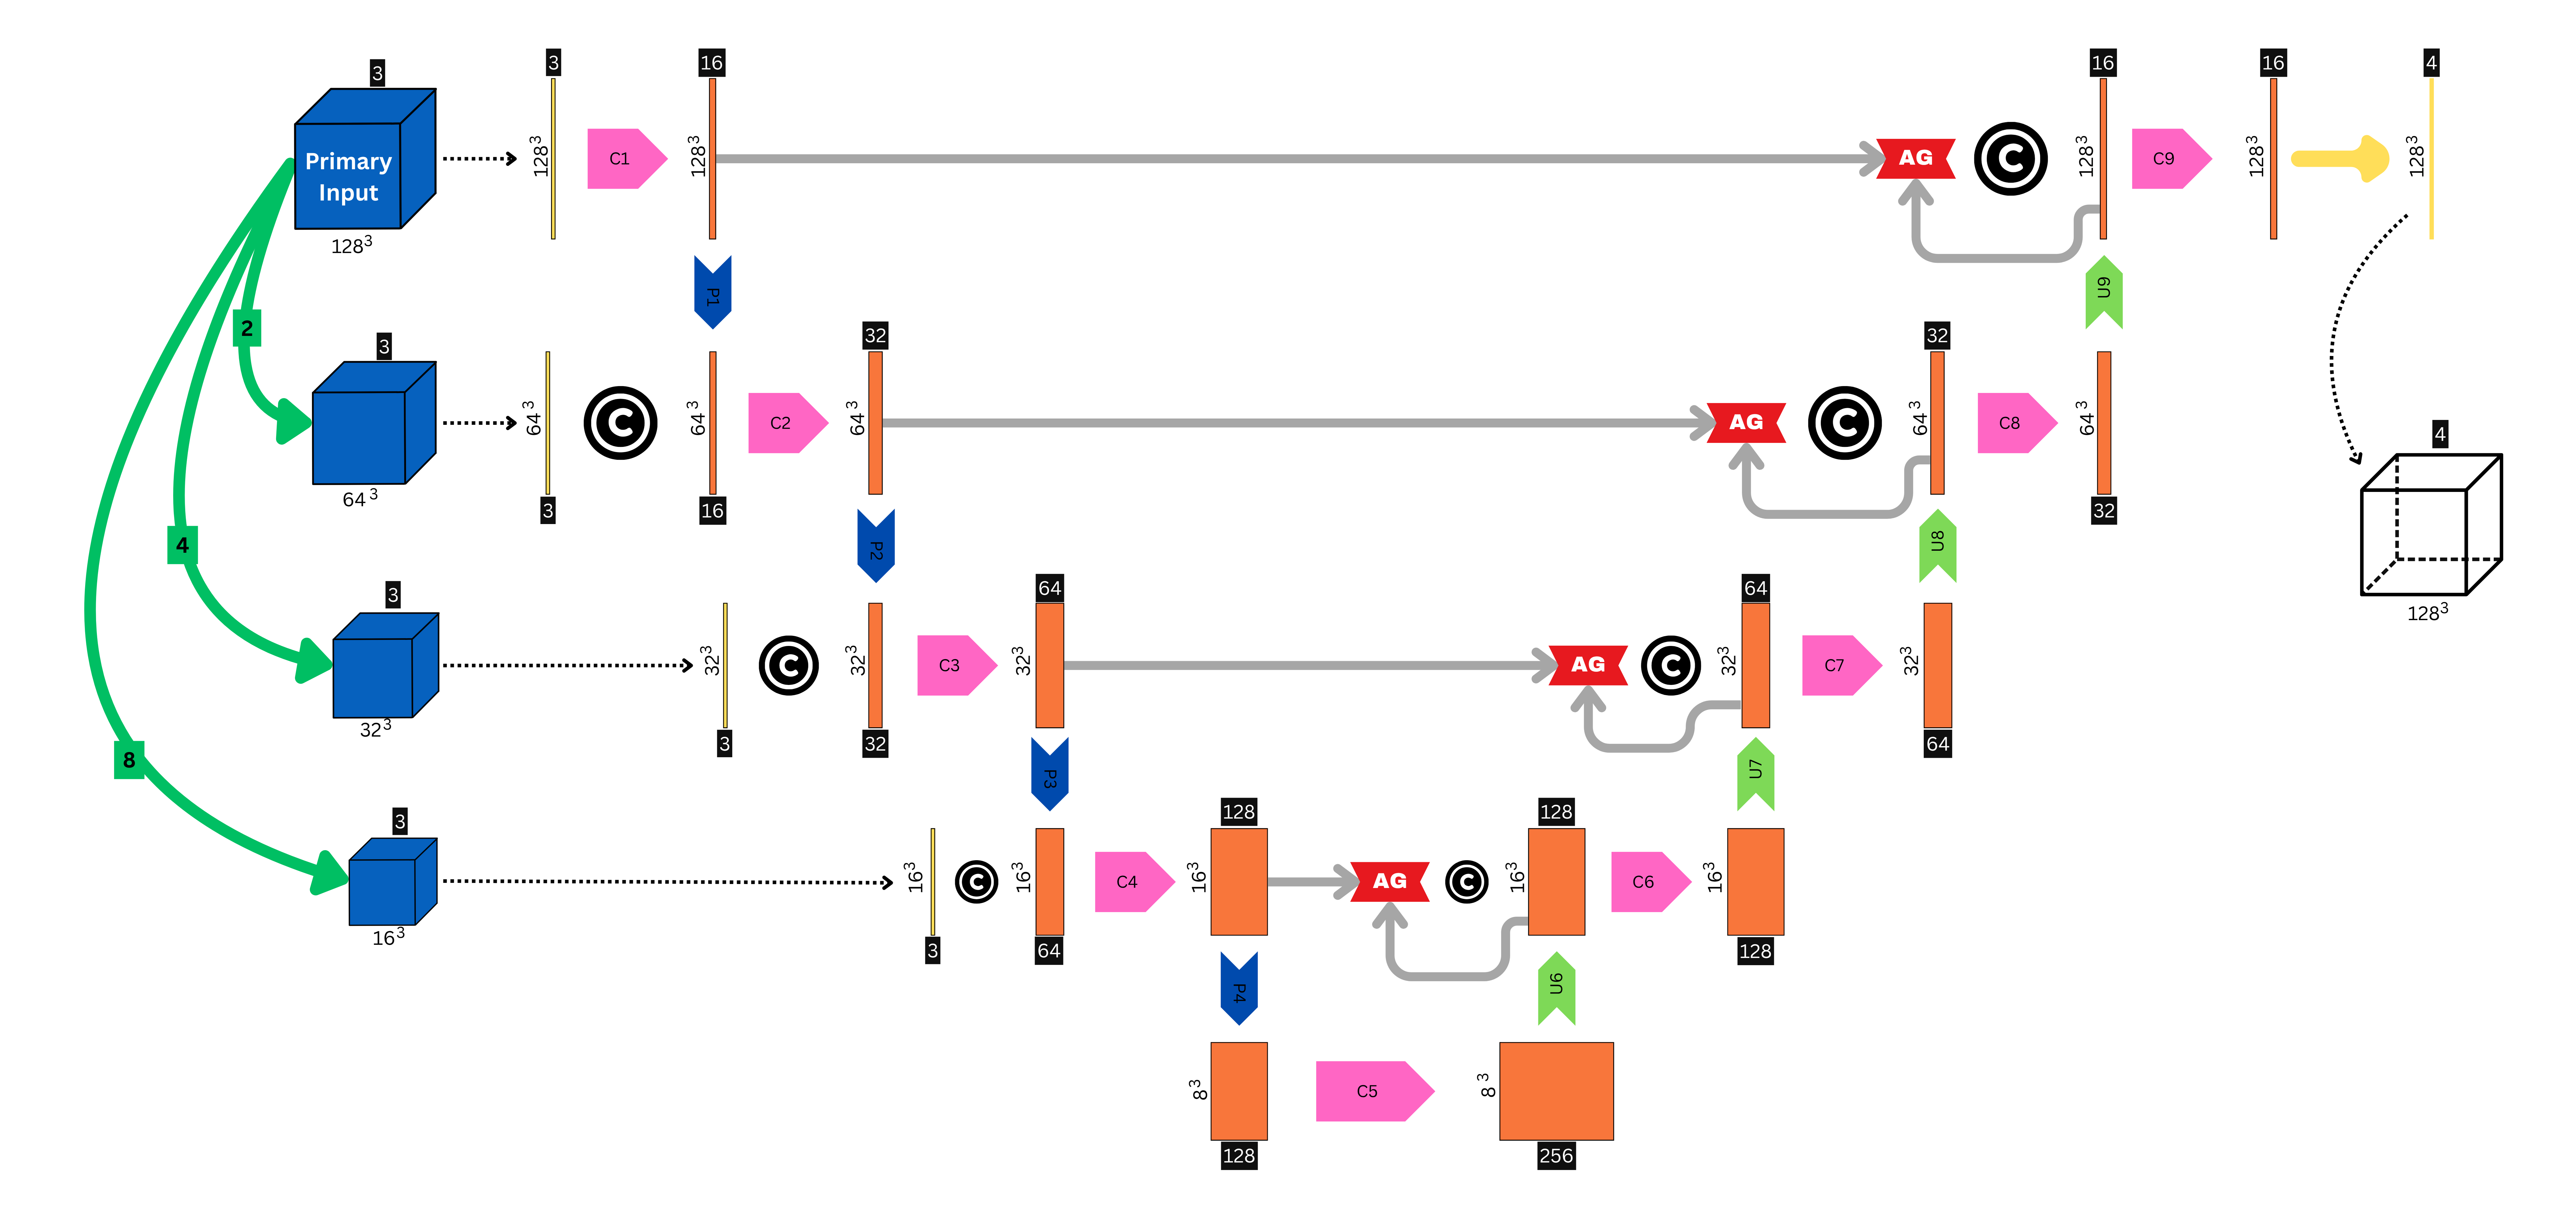
\includegraphics[width=\textwidth]{figs/Overall Architecture.png}

    \vspace{2mm}

    \setlength{\dashlinedash}{0.5pt}
    \setlength{\dashlinegap}{1.5pt}

    \fbox{
    \begin{tabular}{cl|cl|cl}
        
\includegraphics[width=0.018\textwidth]{figs/Label1/1.png}
        & \scriptsize Concatenation
        &
        
\includegraphics[width=0.015\textwidth]{figs/Label1/9.png}
        & \scriptsize MaxPool
        &
        
\includegraphics[width=0.015\textwidth]{figs/Label1/7.png}
        & \scriptsize TransConv
        \\[1.5mm]
        \hdashline
        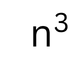
\includegraphics[width=0.030\textwidth]{figs/Label1/3.png}
        & \scriptsize Dimension
        &
        
\includegraphics[width=0.030\textwidth]{figs/Label1/4.png}
        & \scriptsize Number of channels
        &
        
\includegraphics[width=0.030\textwidth]{figs/Label1/8.png}
        & \scriptsize Dense Inception-Res Block
        \\[1.5mm]
        \hdashline
        
\includegraphics[width=0.030\textwidth]{figs/Label1/10.png}
        & \scriptsize AttentionGate
        &
        
\includegraphics[width=0.030\textwidth]{figs/Label1/2.png}
        & \scriptsize Average-pooled by factor of $n$
        &
        
\includegraphics[width=0.030\textwidth]{figs/Label1/11.png}
        & \scriptsize Conc 1x1x1 with sigmoid
    \end{tabular}
    }

    \caption{Integrated Architectural Framework}
    \label{FIG:Overall Architecture}
\end{figure*}

\subsection{Encoder (Contracting Path)}

At each encoder stage $l\in\{1,2,3,4\}$, the network performs three sequential operations:
\begin{itemize}
    \item Feature Extraction (Dense Inception Residual Convolution):
    \begin{itemize}
        \item Each stage applies a DRIC block, combining multiple convolutional branches with different receptive fields
        \item The block output is: $F_l = DRIC_l (X_{l-1})$
    \end{itemize}
    \item Downsampling:
    \begin{itemize}
        \item The feature map is halved in each spatial dimension using 3D max pooling: $X_l = MaxPool3D(F_l,\allowbreak\, p = 2)$, where $p$ represents the scaling factor.
    \end{itemize}
    \item Skip Connection Storage:
    \begin{itemize}
        \item Each pre-pooled feature map $F_l$ is preserved for later fusion with the decoder at the corresponding level.
    \end{itemize}
\end{itemize}

\subsection{Multiscale Input}

The input in the form of numpy array is downsampled through an simple average pooling function that converts the primary input of size $128^3\times3$ into multiple scaled down inputs of $128^3\times3$, $64^3\times3$, and $32^3\times3$; that is then fed to the encoder at different stages.
The original input $X_0$ (of size $128^3\times3$) is successively downsampled:
$\tilde{X}_l=Downsample(X_0,scale=2^l), l$ represents the encoder stage, and concatenated with $X_{l-1}$ before entering the next DRIC block:
$\hat{X}_l=[X_{l-1} \| \tilde{X}_l]$.

\subsection{Bottleneck (Bridge)}

The lowest-level encoder output passes through a bottleneck DRIC block, $B = DRIC_{bottleneck}(X_4)$.

\subsection{Decoder (Expanding Path)}

The decoder path performs progressive upsampling and reconstruction to return the segmentation to full spatial resolution. At each decoder stage $m \in {4,3,2,1}:$

\begin{itemize}
    \item Upsampling:
The feature map is expanded using transposed 3D convolutions: $U_m = ConvTranspose3D\allowbreak(B_m, k = 2, s = 2)$, where $k$ and $s$ denote kernel size and stride, respectively.
\end{itemize}

\begin{itemize}
    \item Attention-Gated Skip Connection:
Before concatenating with its encoder counterpart $F_m$, an attention gate filters the encoder feature map based on relevance to the decoder's context.
Let the gating signal of the decoder be $g_m$ and the encoder feature be $F_m$; the attention coefficient is computed as:
$\alpha_m = \sigma(W_g * g_m + W_x * F_m+b),$ and the refined feature map is: $\tilde{F}_m=\alpha_m \odot F_m,$ where $\odot$ denotes element-wise multiplication. This suppresses irrelevant background and enhances focus on tumor boundaries and salient regions.
\end{itemize}

\begin{itemize}
    \item Fusion and Convolution:
			The attention-refined skip feature $\tilde{F}_mis$ concatenated with $U_m:
    \\C_m=[U_m \| \tilde{F}_m],$ which is then processed by another DRIC block: $B_{m-1} = DRIC_m(C_m)$.
\end{itemize}

\subsection{Output Layer}

After the final decoder stage, a $1 \times 1 \times 1$ convolution projects the feature volume into the four output classes: $Y=Softmax(W_{out} * B_0 + b_{out})$,
where $Y \in [0,1]^{H \times W \times D \times 4}$ represents per-voxel class probabilities for background, NCR/NET, ED, and ET.


%% ============================================================
%% SECTION: Loss Functions
%% ============================================================

\section{Loss Functions}

The choice of an appropriate loss function is critical for medical image segmentation, particularly in highly imbalanced tasks such as brain tumour segmentation, where foreground regions often occupy a very small fraction of the overall volume. In this work, we proposed an Adaptive Loss Function that combines Dice Loss with Categorical Focal Loss, dynamically adjusting their relative contributions as training progresses.

\subsection{Dice Loss}

The Dice coefficient directly measures the overlap between the predicted and ground truth masks. For multi-class segmentation, the Dice Loss is defined as:
\begin{equation}
    \mathcal{L}_{\text{Dice}} = 1 -
    \frac{
        2 \sum_{i=1}^{N} \sum_{c=1}^{C} y_{i,c}\,\hat{y}_{i,c}
    }{
        \sum_{i=1}^{N} \sum_{c=1}^{C} y_{i,c}^{2}
        +
        \sum_{i=1}^{N} \sum_{c=1}^{C} \hat{y}_{i,c}^{2}
        +
        \epsilon
    }
    \label{Dice Loss}
\end{equation}
where $y_{i,c} \in \{0,1\}$ denotes the ground truth one-hot encoded label for voxel $i$ in class $c$, $\hat{y}_{i,c}$ represents the predicted softmax probability, $N$ is the total number of voxels, $C$ is the number of classes, and $\epsilon$ is a small constant added for numerical stability.

Dice Loss encourages overlap between predicted and ground-truth masks, and is particularly effective at handling class~imbalance.

\subsection{Categorical Focal Loss}

To further address the imbalance and focus learning on difficult-to-classify voxels, we employ the Categorical Focal Loss (adapted from Lin et al., 2017):
\begin{equation}
    \mathcal{L}_{\text{Focal}} = - \frac{1}{N}
    \sum_{i=1}^{N} \sum_{c=1}^{C}
    \alpha_c \left(1 - \hat{y}_{i,c}\right)^{\gamma}
    \, y_{i,c} \log\left(\hat{y}_{i,c}\right)
\end{equation}
Here, $\gamma > 0$ is the focusing parameter that reduces the relative loss contribution of well-classified voxels, while $\alpha_c$ is the balancing factor for class $c$.

\subsection{Adaptive Weighting Strategy}

Rather than fixing the relative importance of Dice and Focal losses, we introduce a dynamic weighting scheme that changes over epochs. Let $t$ denote the current epoch, then the weights are defined as:
\begin{equation}
    w_{\text{Dice}}(t) = \frac{1}{1 + \exp(-\beta t)},
    \quad
    w_{\text{Focal}}(t) = 1 - w_{\text{Dice}}(t).
\end{equation}
Where $\beta$ controls the smoothness of the transition. Early in training, the model emphasizes Focal Loss to tackle hard examples and improve class discrimination. As training progresses, the weight shifts towards Dice Loss, ensuring that fine-grained segmentation quality and overlap improve.

\subsection{Combined Loss}

The final adaptive loss is then given by:
\begin{equation}
    \mathcal{L}_{\text{Adaptive}}(t) =
    w_{\text{Dice}}(t)\, \mathcal{L}_{\text{Dice}}
    +
    w_{\text{Focal}}(t)\, \mathcal{L}_{\text{Focal}}
\end{equation}


%% ============================================================
%% SECTION: Results and Discussions
%% ============================================================

\section{Results and Discussions}

This adaptive scheme enables a balanced optimization process, starting with robust class-level discrimination and gradually shifting toward maximizing spatial overlap between predicted and ground truth tumour regions.

\begin{figure*}[!htbp]
    \centering
    \begin{subfigure}[b]{0.48\textwidth}
        \centering
        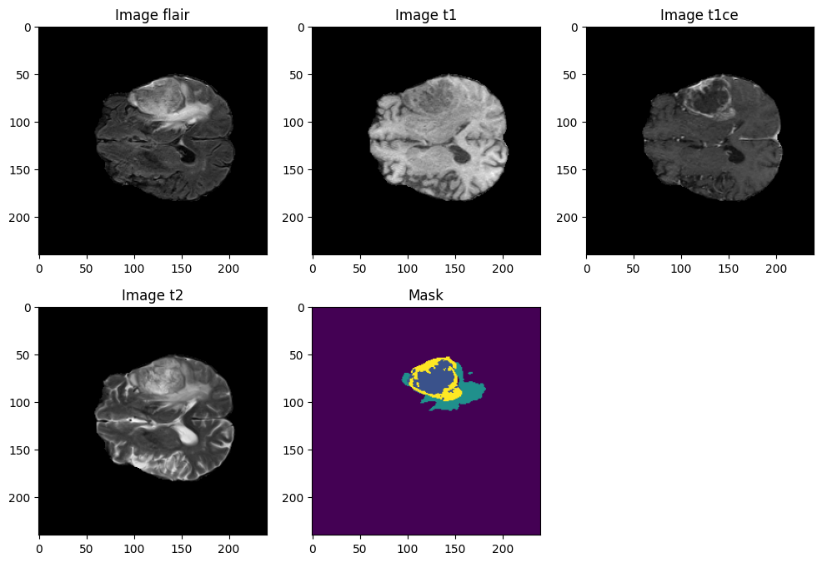
\includegraphics[width=\linewidth]{figs/Dataset Prep Img1.png}
        \caption{Uncropped Data}
        \label{fig:segA}
    \end{subfigure}
    \hfill
    \begin{subfigure}[b]{0.48\textwidth}
        \centering
        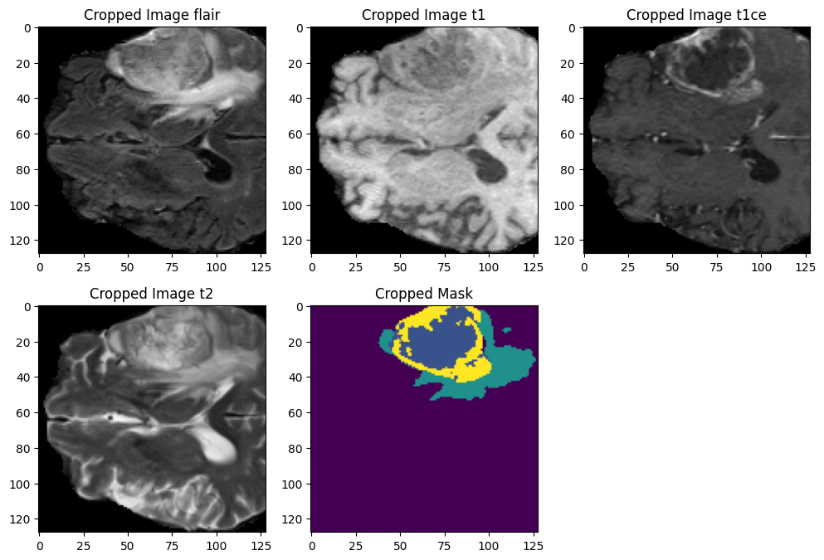
\includegraphics[width=\linewidth]{figs/Dataset Prep Img2.png}
        \caption{Cropped Data}
        \label{fig:segB}
    \end{subfigure}
    \caption{Visual comparison demonstrating the impact of cropping in the worst-case scenario, namely at the middle slice where the brain occupies its maximum cross-sectional area.}
    \label{fig:wide}
\end{figure*}

\subsection{Experimental Setup}

\subsubsection{Data Pre-processing and Training}

For Training we have used the Data from the popular BraTS Dataset, modifying it slightly to our convenience. In the BraTS Dataset, each image consists of four modalities. These modalities are essentially different representations of the same brain image but containing different types of information as they are captured through different criterion. These modalities are called T1, T1CE(T1 Contrast Enhanced), T2, and Flair. All the modalities for each date are present in the dataset in the form of .nii flies, along with the ground-truth mask which is also present in .nii file format. For processing this data prior to training we excluded the T1 modality, as T1CE is just the contrast enhanced version of T1, as it contains most of the information present in T1 while additionally providing contrast-enhanced information due to it being contrast enhanced. This means we can reduce 25\% size for each data while loosing little to no useful information. For the remaining 3 modalities(T1CE, T2 and Flair) we first cropped each modality from a size of $240\times240\times155$ to $128\times128\times128$. Now theoretically this may also lead to loosing so essential information from the data. However, even after hard cropping, we still retain almost all the image information. This is shown in Fig.~\ref{fig:wide}

In this we are seeing exactly the middle slice of an example data. Being the middle slice, this is the worst case scenario of how the crop affects the data, as the brain cannot be any wider in any other portion. As even in the widest part of the brain more than 90\% of the data is still present, and almost all off the ground truth mask is present. This suggests that that >97\% of the useful data is still present. Through cropping, we are discarding the black empty portion around the brain, making the date more light weight and easier to handle. this trade-off was considered acceptable due to the negligible impact on segmentation performance as even if we feed the model uncropped data afterwords when the training is done, it predicts the ground truth mask with effectively the same accuracy. This cropping strategy was also beneficial as it brings the size of each dimension in the order of $2^n$, which is consider to be the best practice for any data that is being fed to a network with multiple maxpooling layers. These .nii files are then converted into numpy arrays of size $128\times128\times128\times3$ and stored on the hard disk as .npy files.

For the ground truth masks they consist four labels: Unlabelled volume (Label 0), Necrotic and non-enhancing tumour core (NCR/NET) (Label 1), Peritumoral edema (ED) (Label 2), GD Enhancing Tumour (ET) (Label 4). Now the ground truth masks have a problem. The ET is ladled as 4 and label 3 is empty. Even though it is not supposed to cause any problems in the training, but just to mitigate the inconsistency, while processing we reassign the ET region from label 4 to label 3 and the data points in the mask files are then one hot encoded and stored as int8 in a numpy array. We store that numpy array in the hard disk as .npy file to use during training.

Another preprocessing step we take is to discard the data where less than 1\% of the volume is covered by the mask, meaning if a data has less than 1\% tumour volume, then we discard that data point entirely\footnote{This discarding criterion, along with the on-the-fly data generator pipeline, is adopted from the YouTube tutorial series by Dr. Sreenivas Bhattiprolu (``Digital Srini'' on YouTube).}.

We combined the BraTS 2020 and BraTS 2021 datasets to obtain a lager dataset. About 1400+ volumetric scan were present in the combined dataset; after applying this discarding criterion, $\sim1200$ valid image-mask pairs remain. The mean file size of a NumPy files for a single image array is approximately 64MB, and the corresponding mask array occupies roughly 48MB. During training, the data are read on-the-fly via a Python generator, which yields a tuple $(X,Y); X,Y$ being an image-Mask pair. This approach avoids loading the entire dataset into memory and makes it possible to train with batch size of $1$ to $3$. The generator also performs random shuffling of the dataset at the beginning of each epoch\footnote{The epoch-wise random shuffling strategy is also adopted from the YouTube tutorial series by Dr.\ Sreenivas Bhattiprolu (``Digital Srini'' on YouTube).}.

For training and development, we utilized multiple GPUs depending on availability, including RTX 3060 Ti Mobile (8 GB VRAM), Titan X Pascal (12 GB VRAM), Quadro P5000 (16 GB VRAM) and Tesla T4 GPU on Google Colab(16GB VRAM). Due to the limitations of the older Quadro P5000 architecture, we faced some problems in handling the computational demands of 3D convolutions. To mitigate memory constraints across all devices, we adopted mixed precision training, which reduces tensor size and thereby alleviates VRAM usage. Even with this optimization, the maximum feasible batch size across all GPUs was limited to 2, the 3060 Ti Mobile had to use a batch size of 1. Approximate GPU VRAM Usage is $\sim11$ GiB for a batch Size of 2 and $\sim13.5GiB$ for a Batch Size of $3$. Average inference times per batch are $0.8853$s and $1.3295$s for a $2$-volume batch and a $3$-volume batch respectively; Average inference times per volume are $0.4427$s and $0.4432$s for a $2$-volume batch and a $3$-volume batch respectively\footnote{VRAM usage and inference times are reported from partial test runs on Google Colab using a Tesla T4 GPU.}.

The hyperparameters for the training are as reported below\footnote{Hyperparameters reported as per the final training run.}:
\begin{itemize}
    \item Learning Rate: $0.0001$
    \item Optimizer: Adam
    \item Epochs: $150$
    \item Batch Size: $2$
\end{itemize}

For the loss function, we used an adaptive combination of Dice Loss and Categorical Focal Loss.

\begin{table*}[!htbp]
    \caption{Validation Performance Summary}
    \label{tbl1}
    \centering
    \small
    \begin{tabular}{lll}
        \toprule
        \makecell[l]{Metric\\(Validation)} &
        \makecell[c]{Best\\(Value, Epoch)} &
        \makecell[c]{Final\\(Value, Epoch)} \\
        \midrule
        \makecell[l]{Validation loss\\(lower is better)} & \makecell[c]{0.130518 (142)} & \makecell[c]{0.138168 (152)} \\
        \makecell[l]{Validation accuracy}                & \makecell[c]{0.988855 (90)}  & \makecell[c]{0.987859 (152)} \\
        \makecell[l]{Mean IoU\\(one-hot mean)}           & \makecell[c]{0.592392 (149)} & \makecell[c]{0.584321 (152)} \\
        \makecell[l]{IoU score}                          & \makecell[c]{0.824554 (142)} & \makecell[c]{0.795915 (152)} \\
        \makecell[l]{F1 score}                           & \makecell[c]{0.962600 (104)} & \makecell[c]{0.927219 (152)} \\
        \makecell[l]{Precision}                          & \makecell[c]{0.969964 (80)}  & \makecell[c]{0.943784 (152)} \\
        \makecell[l]{Recall}                             & \makecell[c]{0.974056 (114)} & \makecell[c]{0.911534 (152)} \\
        \makecell[l]{Dice (TC)$^*$}                      & \makecell[c]{0.983462 (104)} & \makecell[c]{0.958690 (152)} \\
        \makecell[l]{Dice (WT)$^*$}                      & \makecell[c]{0.946574 (145)} & \makecell[c]{0.845925 (152)} \\
        \makecell[l]{Dice (ET)$^*$}                      & \makecell[c]{0.953780 (142)} & \makecell[c]{0.905504 (152)} \\
        \makecell[l]{Macro Dice (average)}               & \makecell[c]{0.950610 (104)} & \makecell[c]{0.903373 (152)} \\
        \bottomrule
    \end{tabular}
    \par\vspace{4pt}
    \parbox{0.6\linewidth}{\footnotesize $^*$TC - Necrotic and non-enhancing tumour core (Label 1); WT - Peritumoral edema (Label 2); ET - GD Enhancing Tumour (Label 3).}
\end{table*}

\begin{figure*}[!htbp]
    \centering
    \begin{tabular}{ccc}
        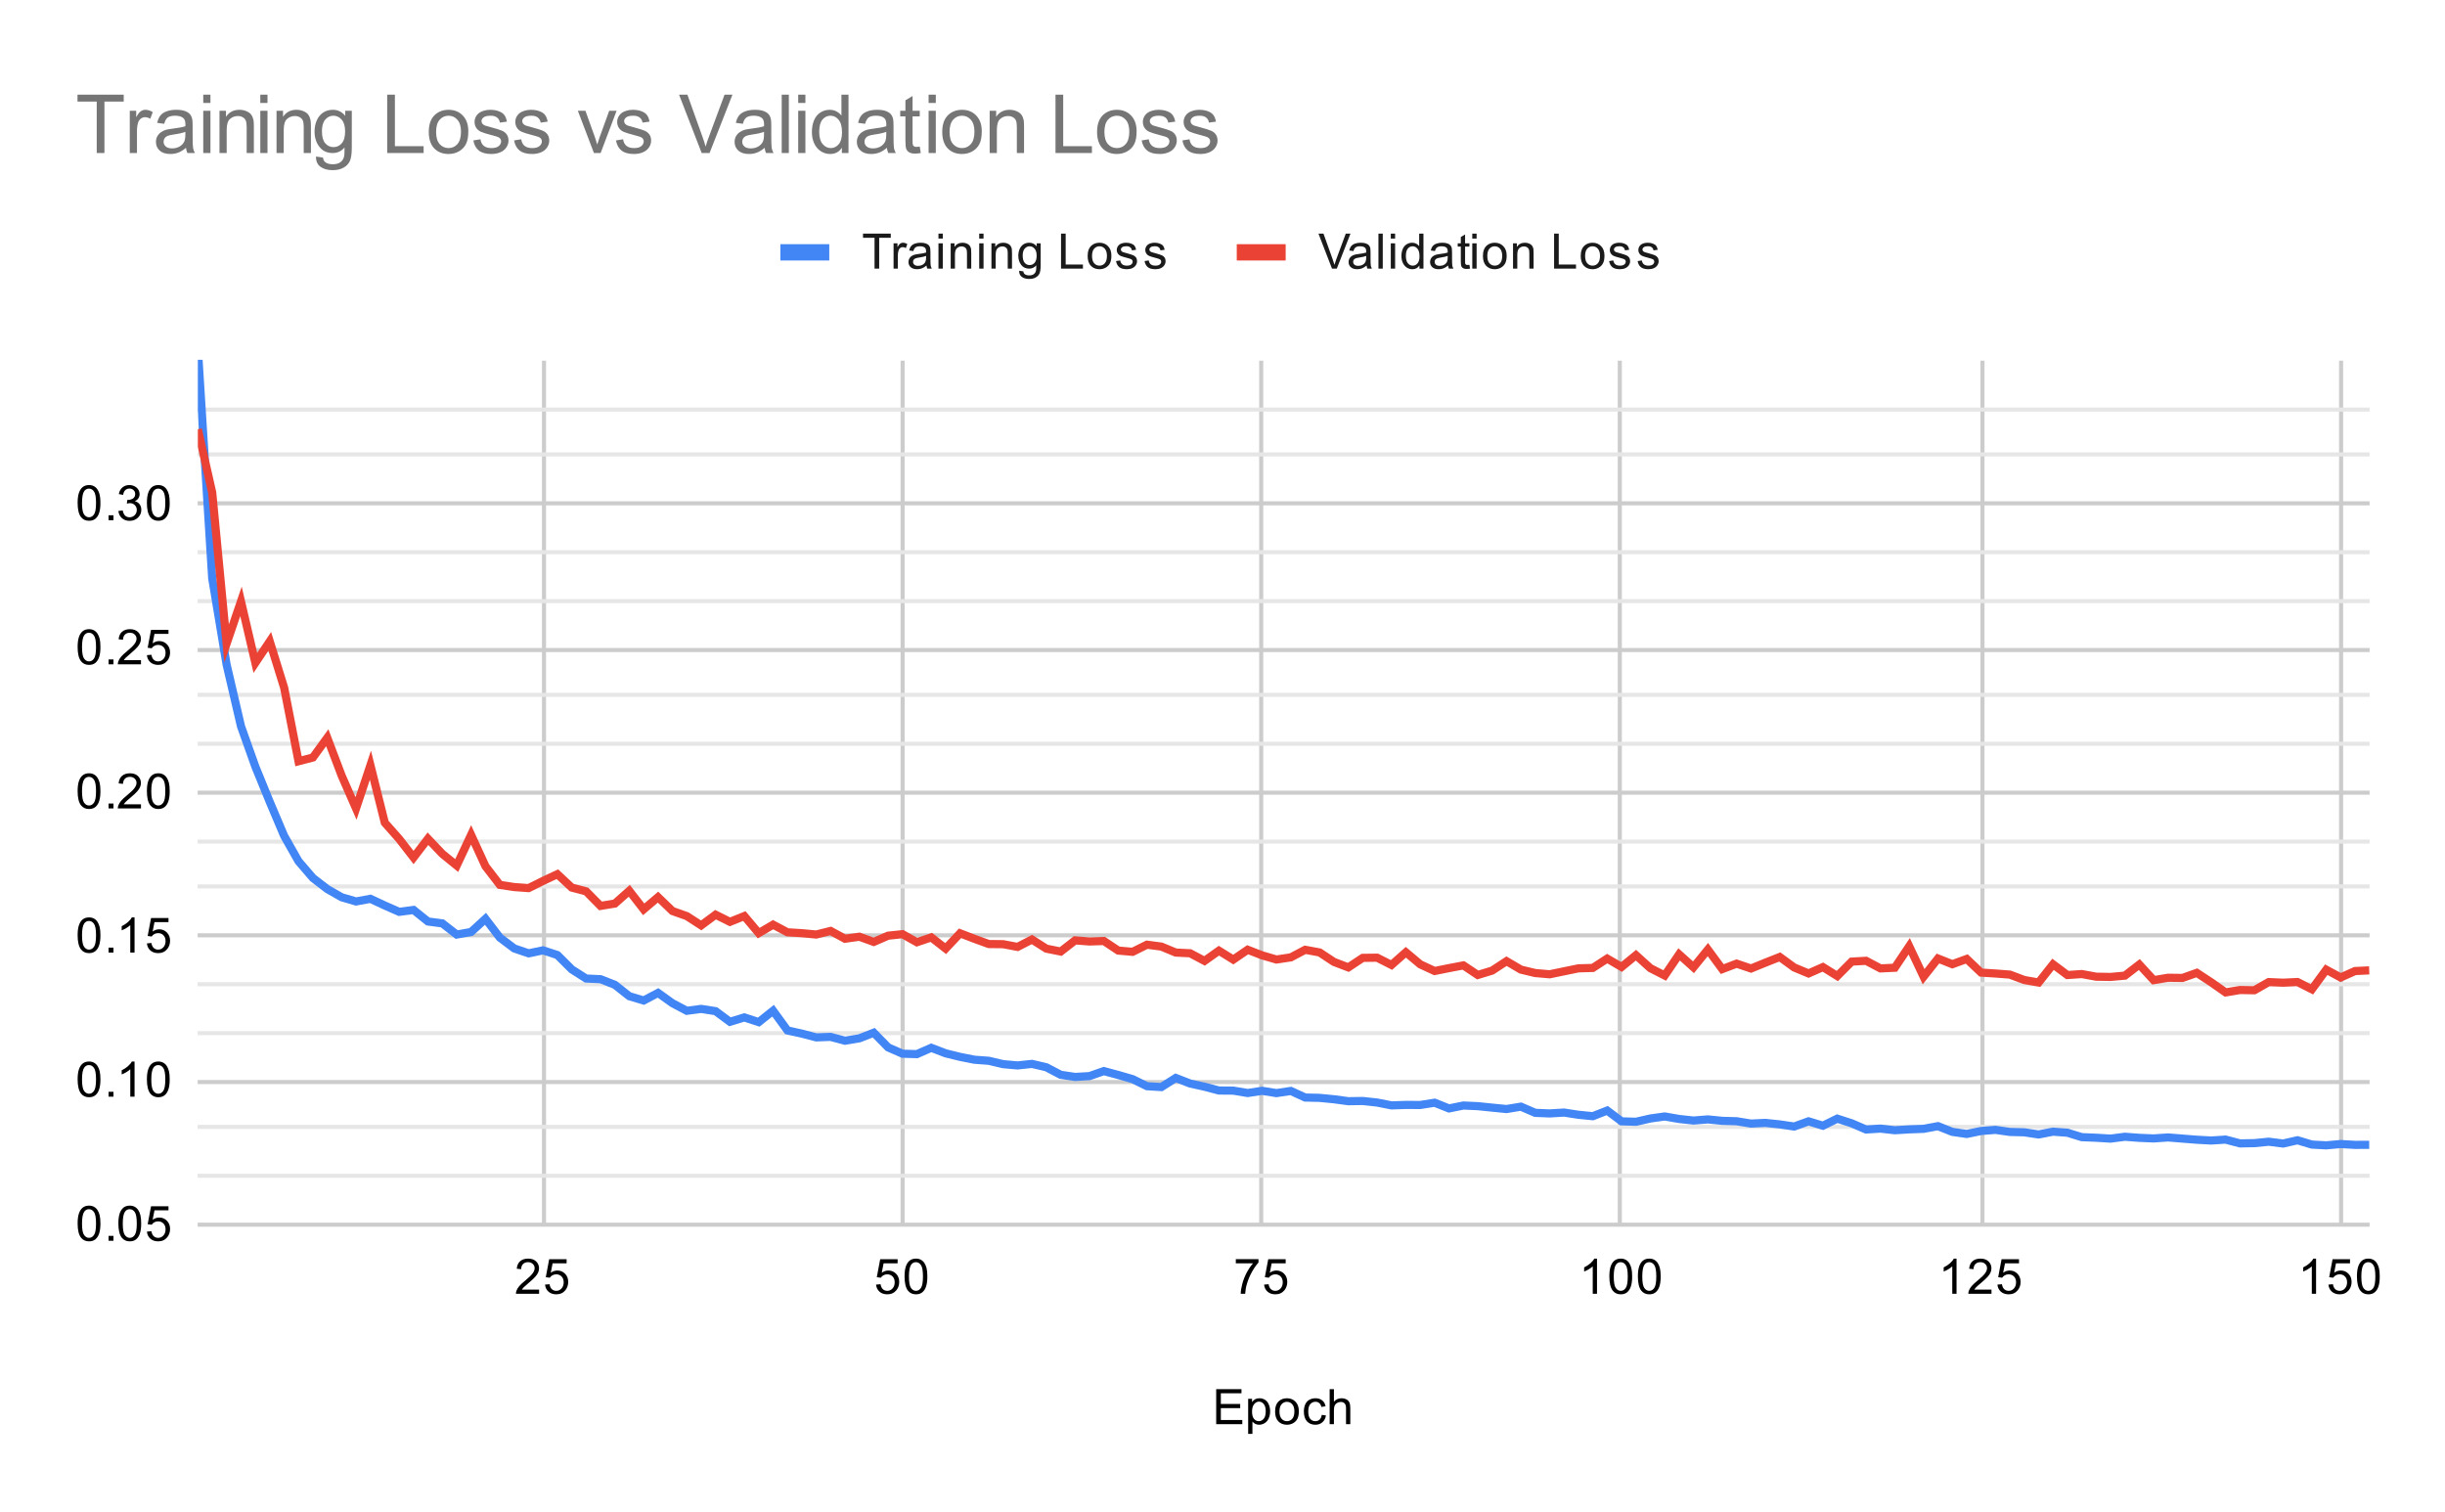
\includegraphics[width=0.3\textwidth]{figs/Project Charts/Training Loss vs Validation Loss.jpg} &
        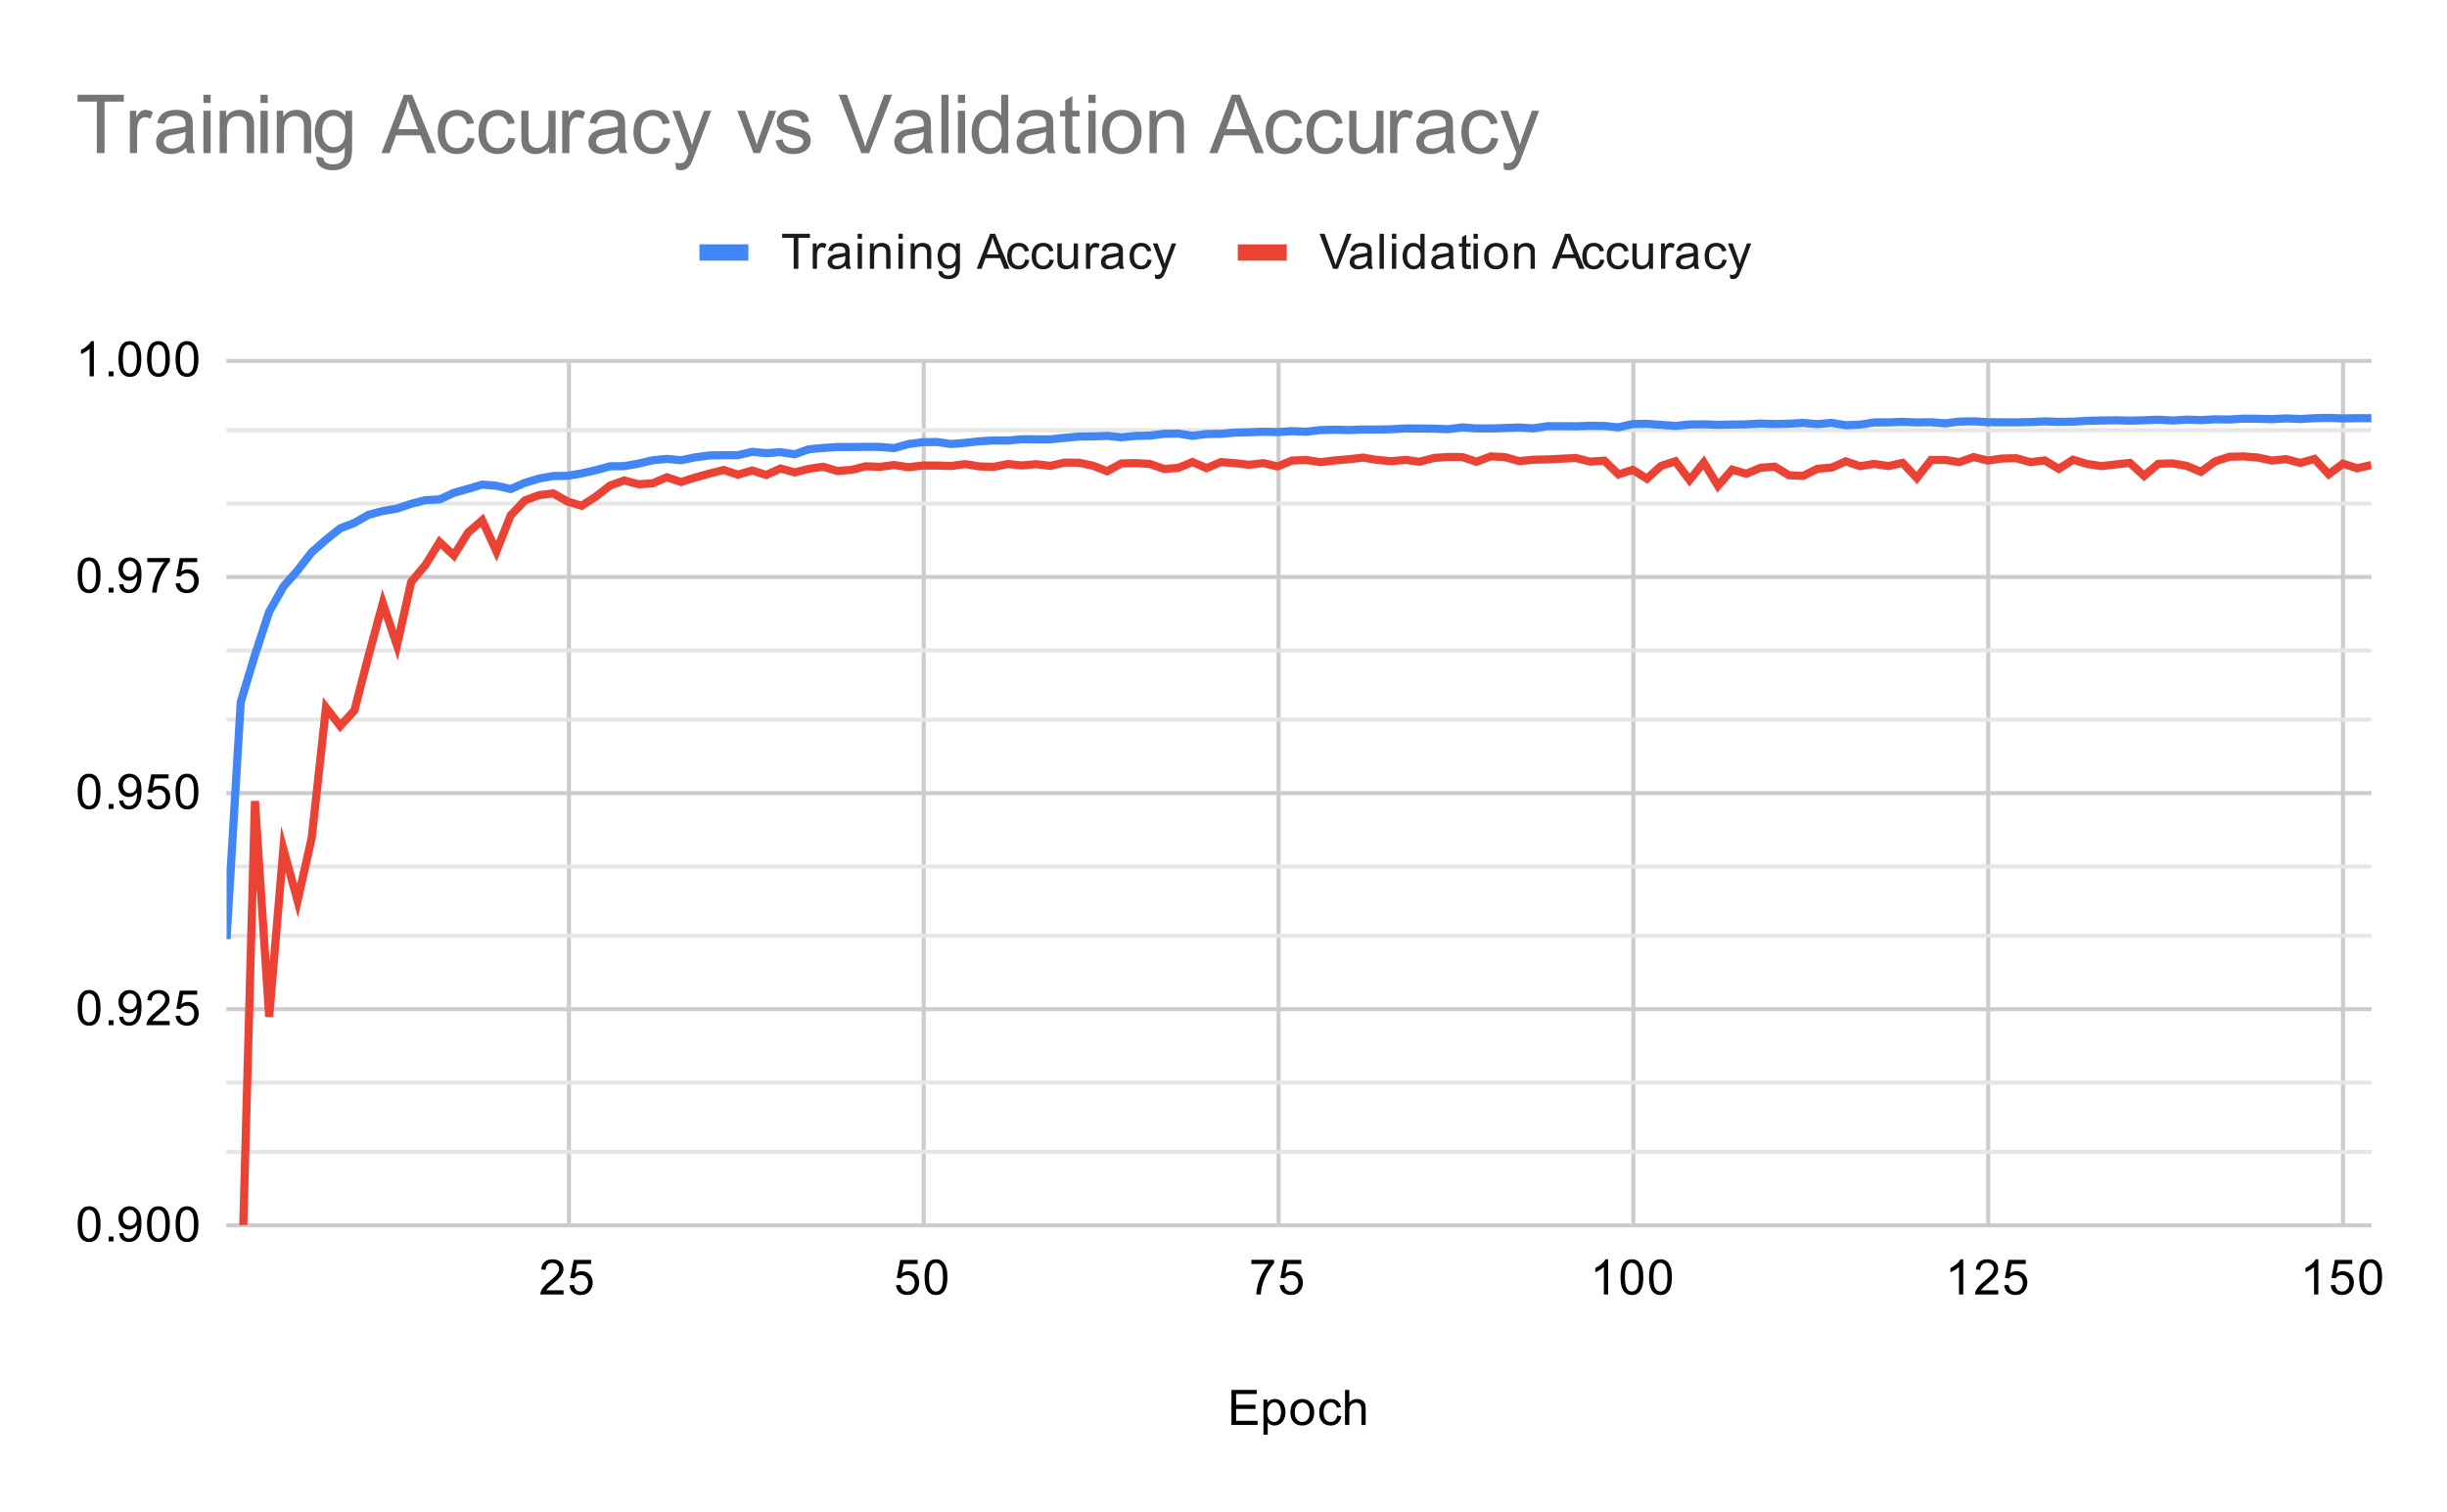
\includegraphics[width=0.3\textwidth]{figs/Project Charts/Training Accuracy vs Validation Accuracy.jpg} &
        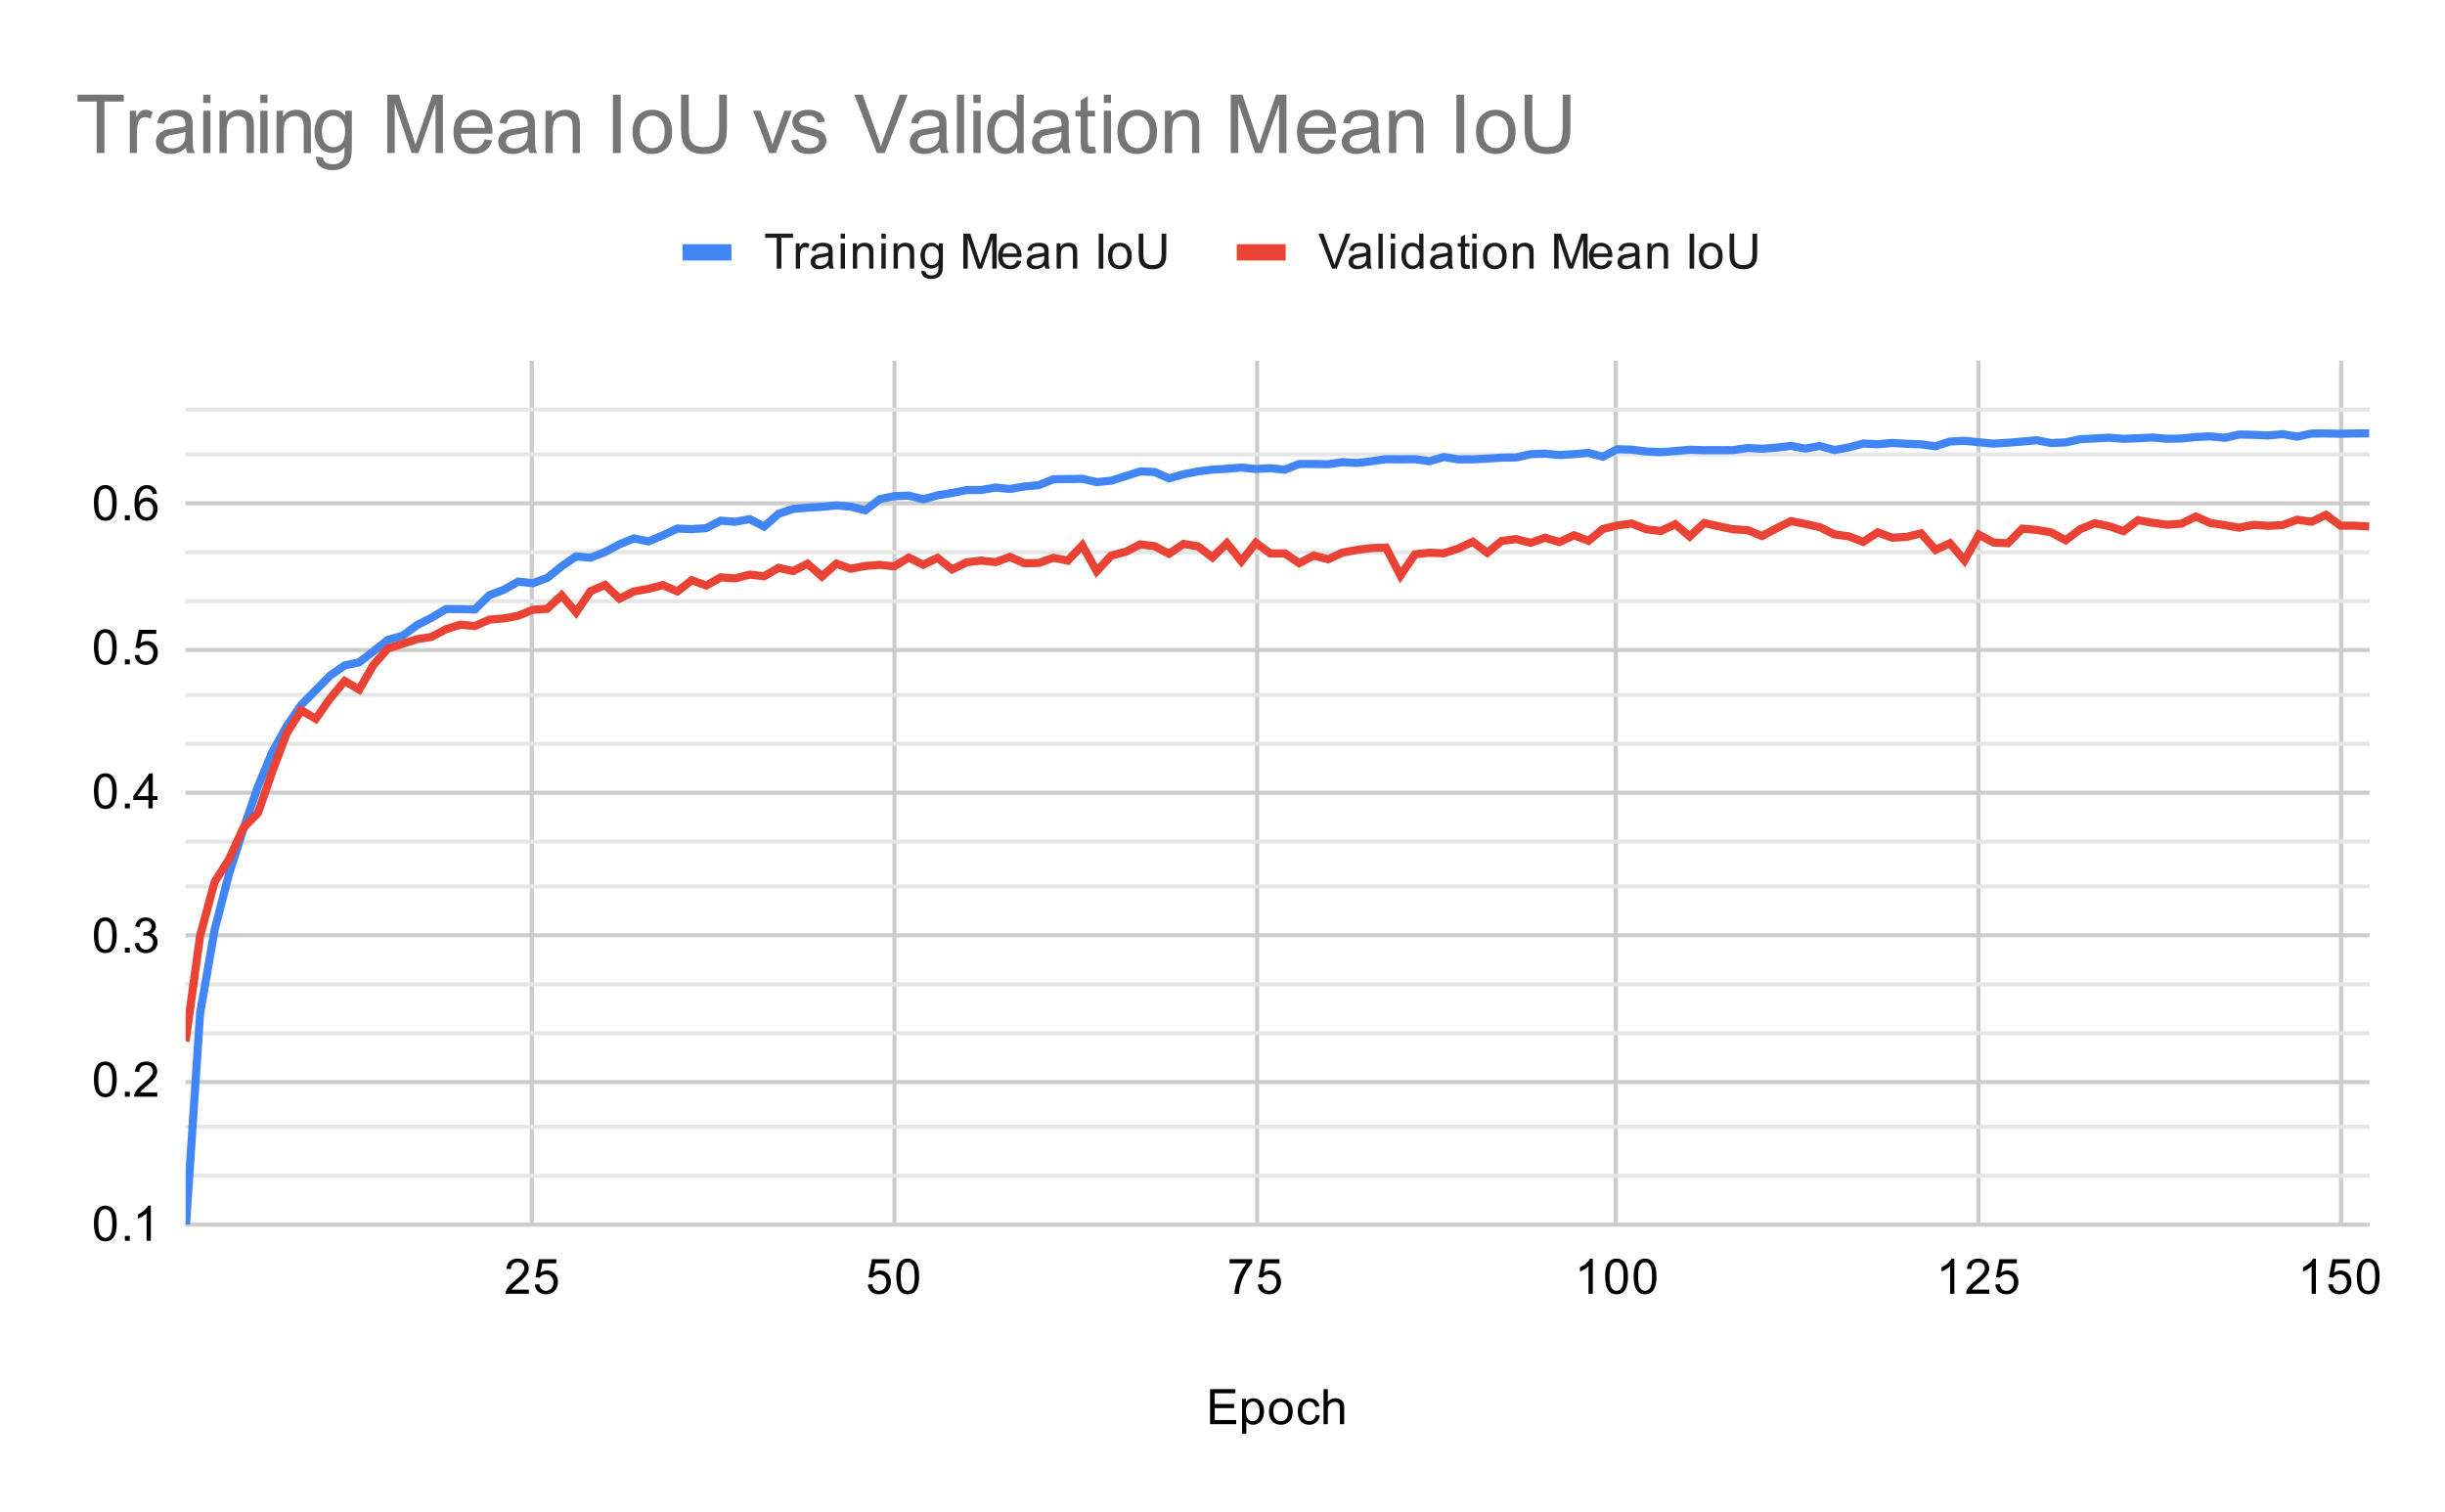
\includegraphics[width=0.3\textwidth]{figs/Project Charts/Training Mean IoU vs Validation Mean IoU.jpg} \\
        (a) Loss Graph & (b) Accuracy Graph & (c) Mean IoU Graph \\[6pt]

        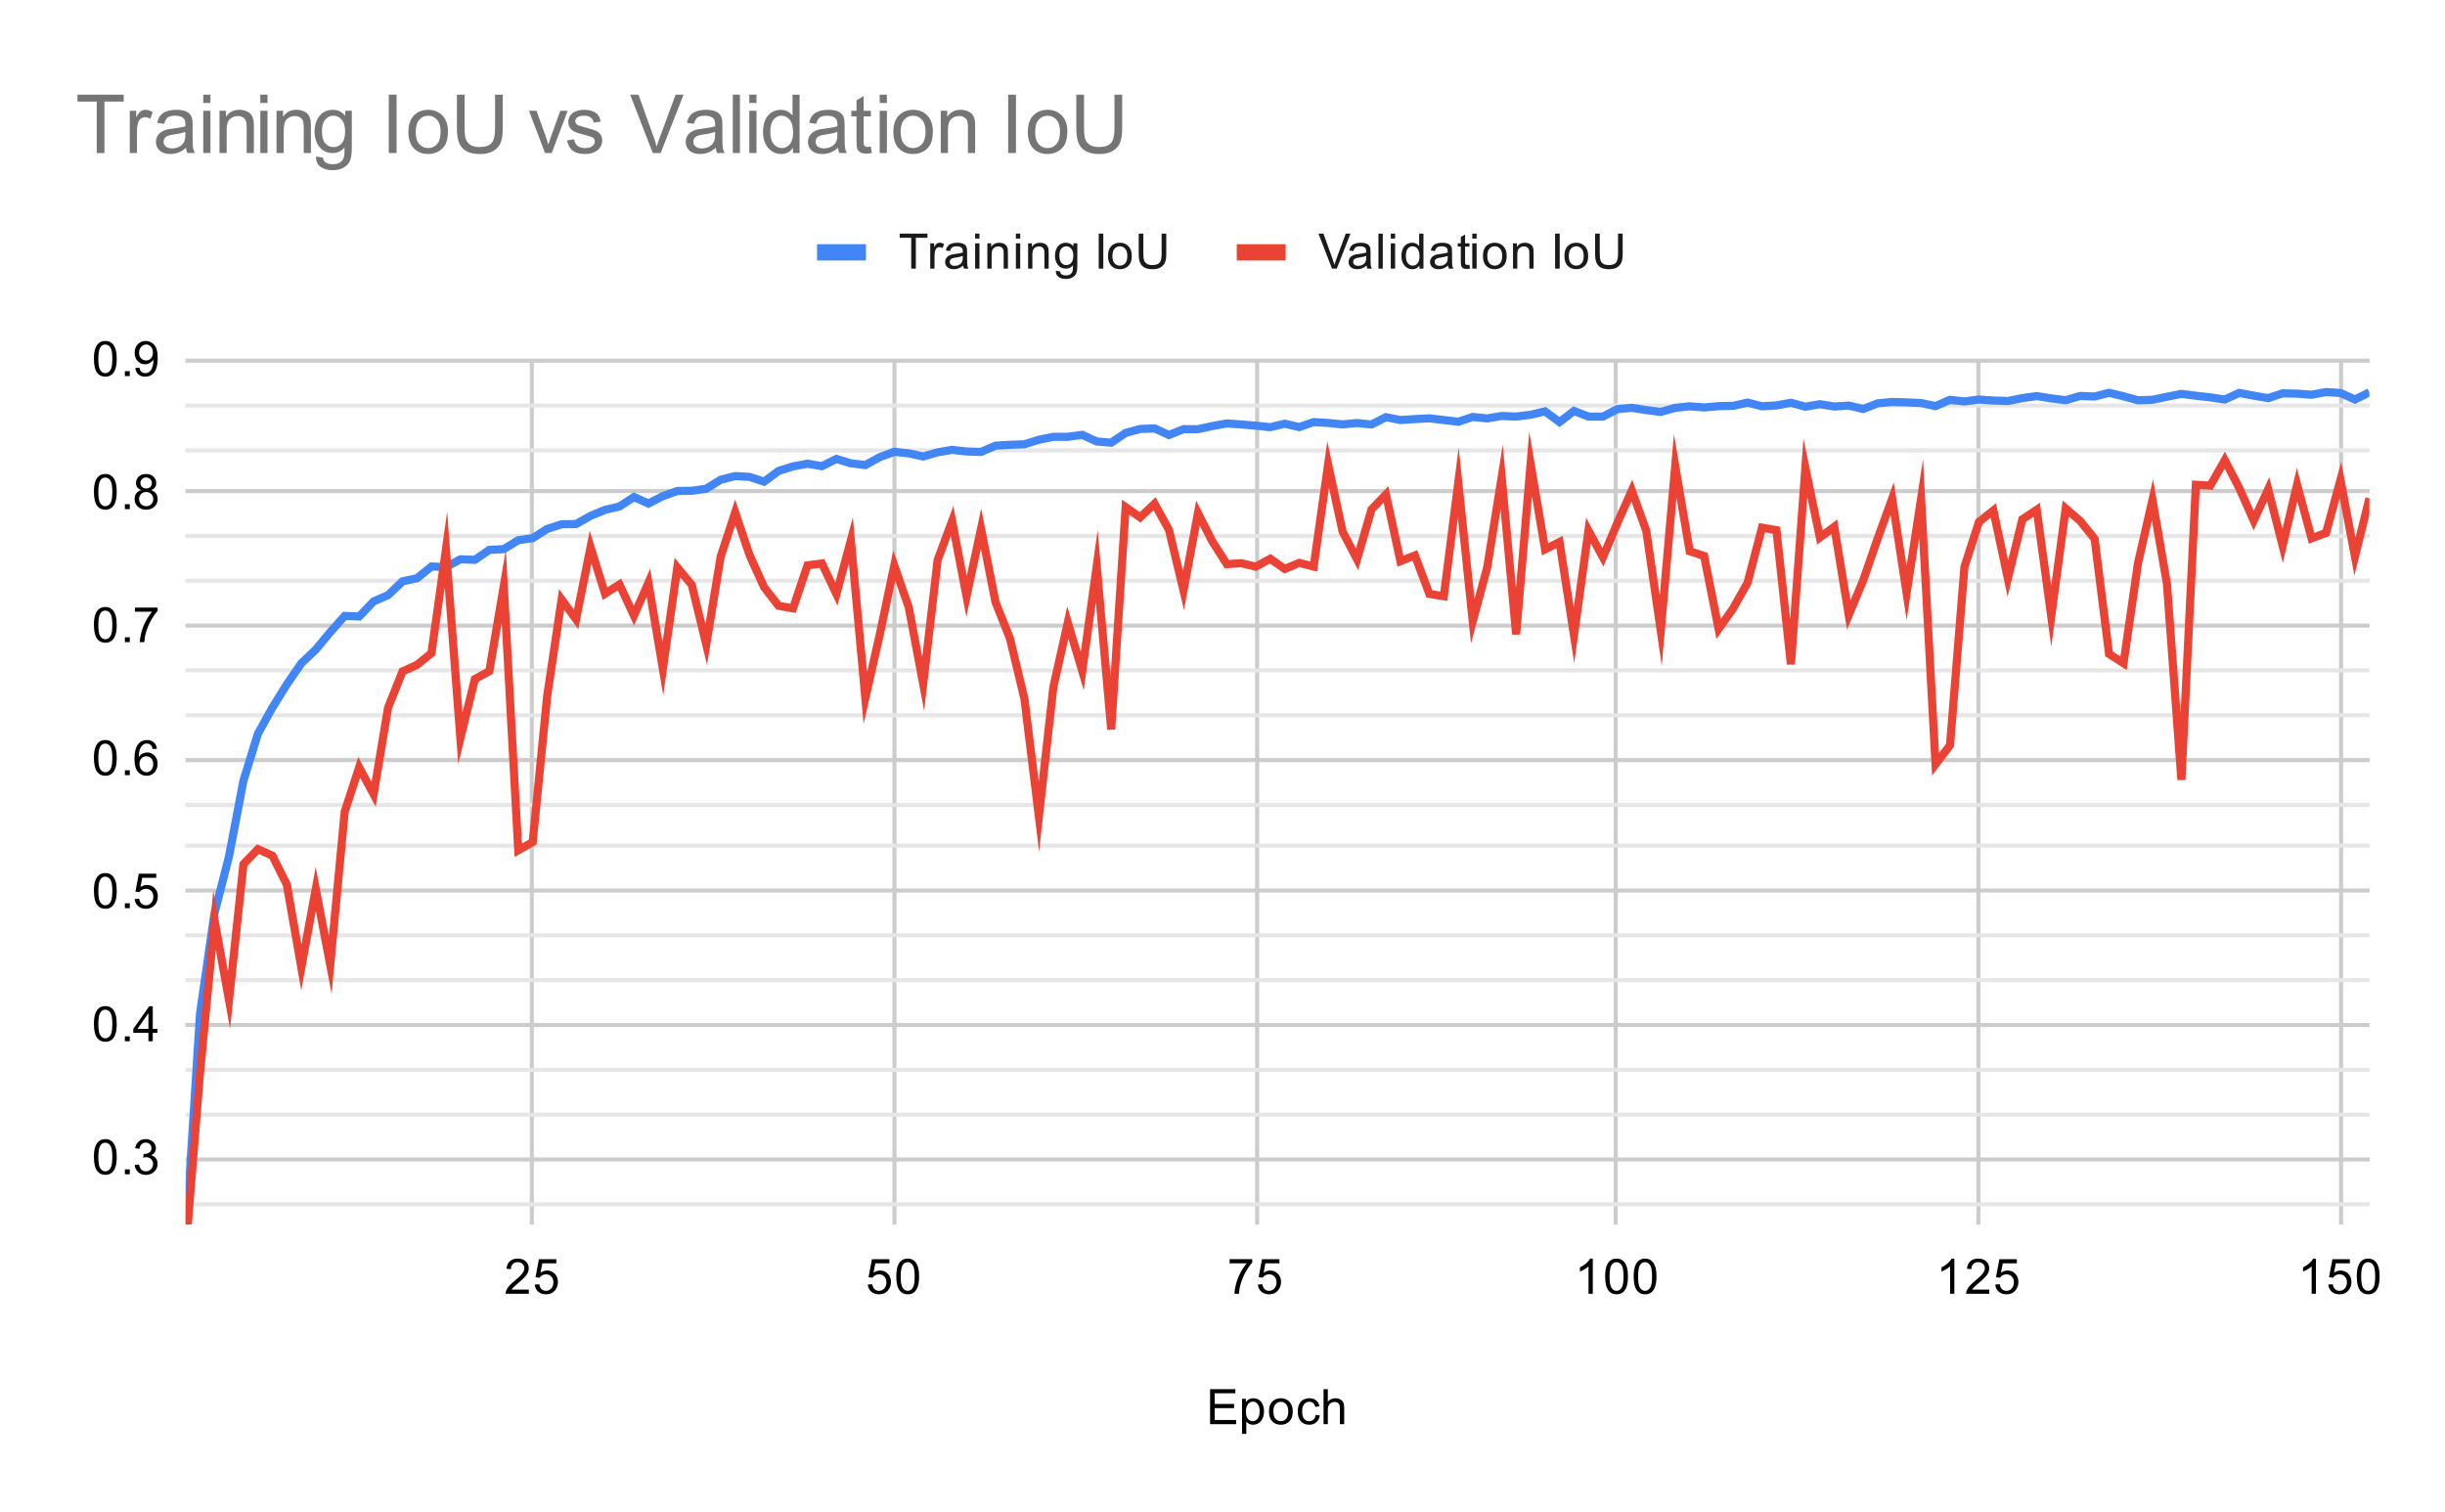
\includegraphics[width=0.3\textwidth]{figs/Project Charts/Training IoU vs Validation IoU.jpg} &
        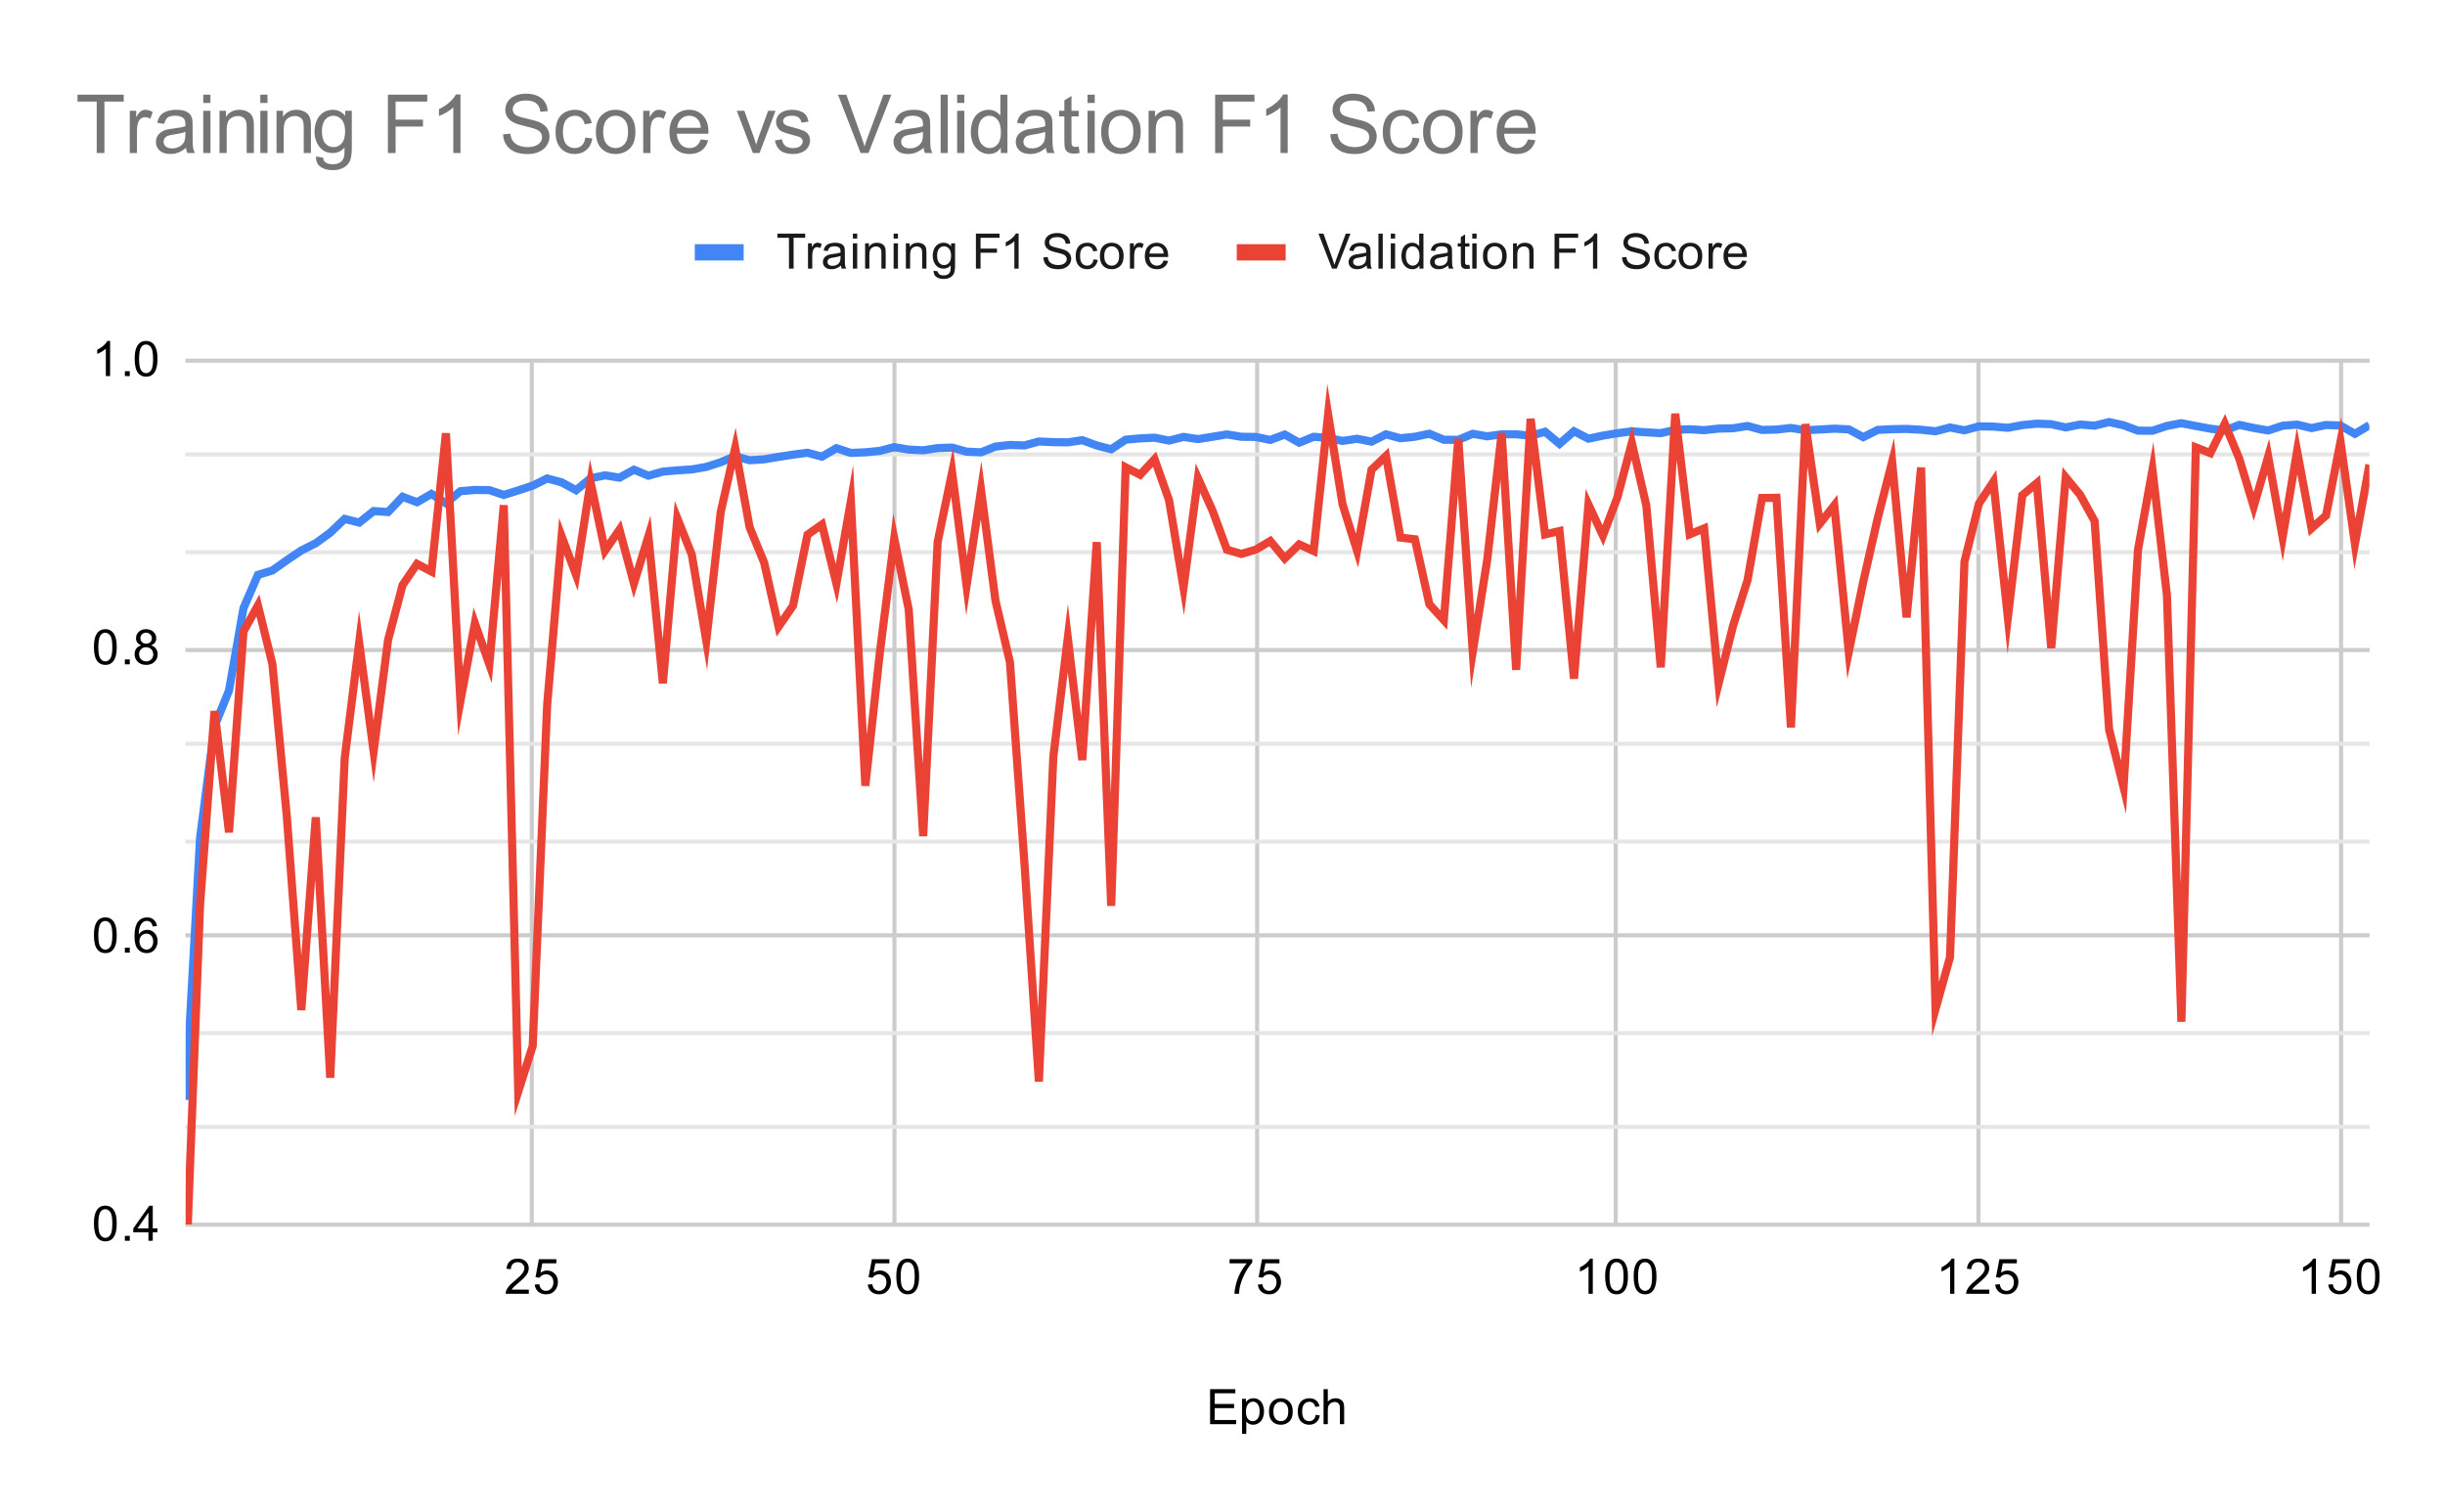
\includegraphics[width=0.3\textwidth]{figs/Project Charts/Training F1 Score vs Validation F1 Score.jpg} &
        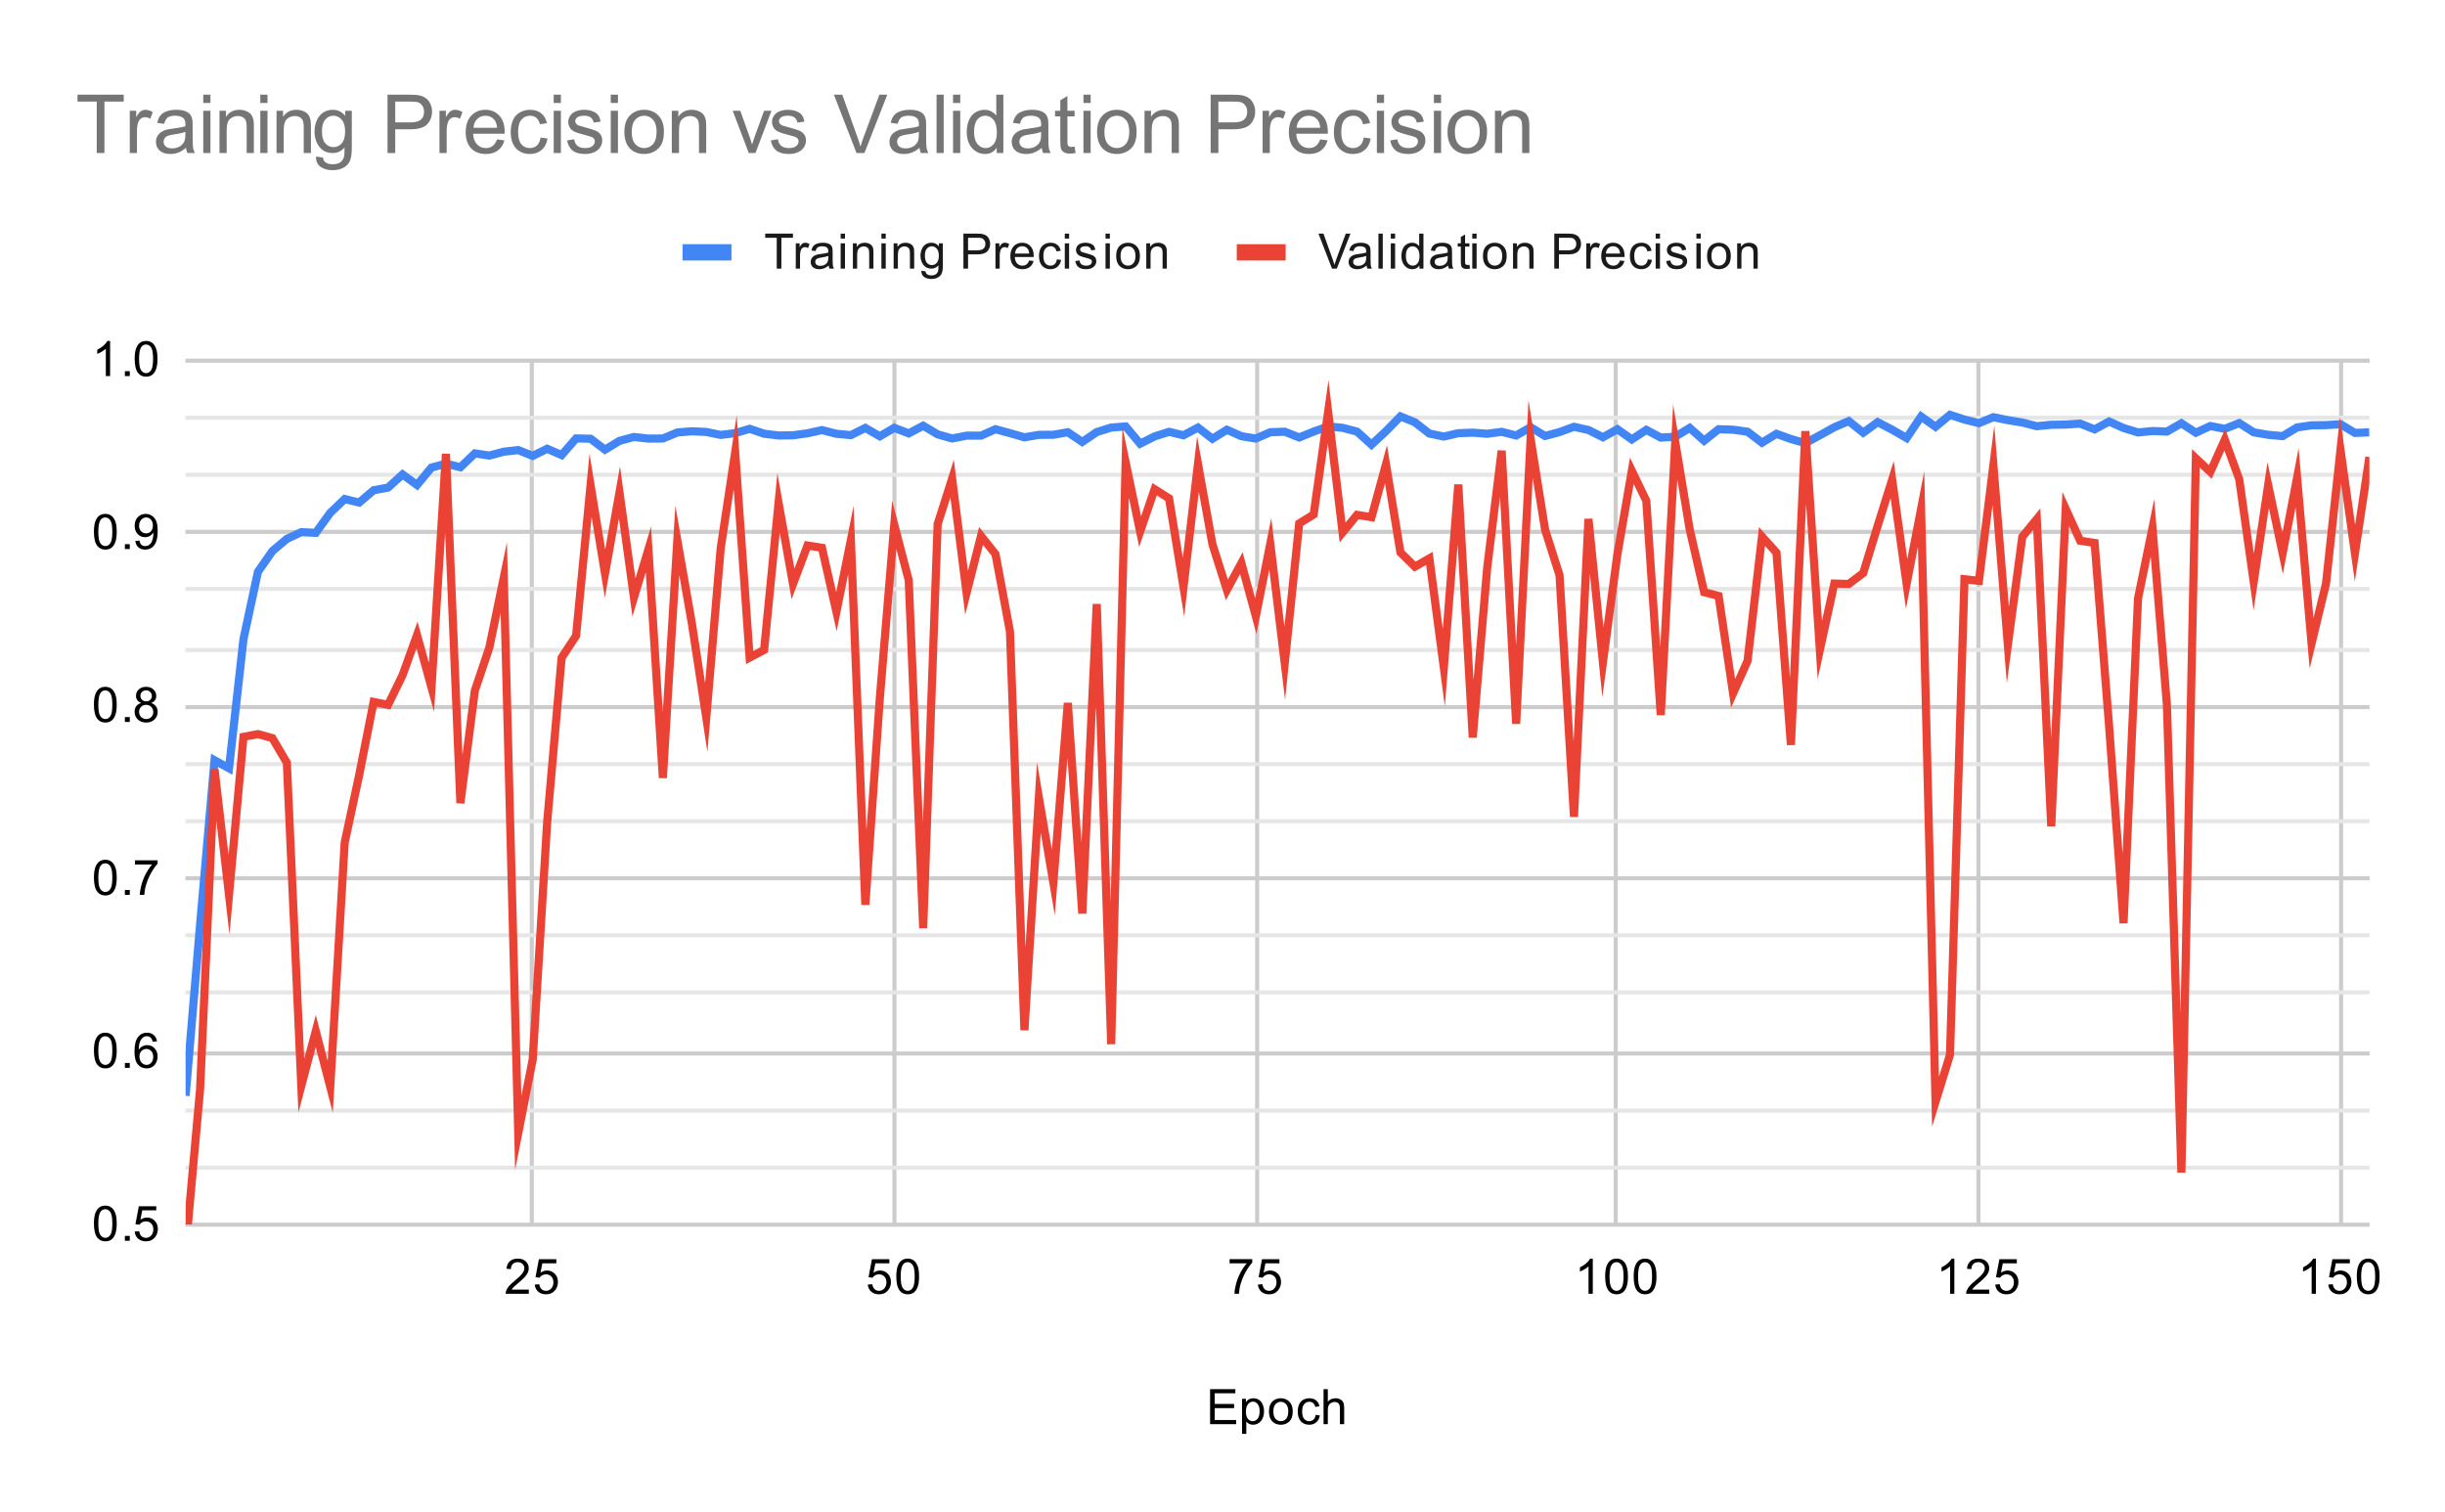
\includegraphics[width=0.3\textwidth]{figs/Project Charts/Training Precision vs Validation Precision.jpg} \\
        (d) IoU Graph & (e) F1 Score Graph & (f) Precision Graph \\[6pt]

        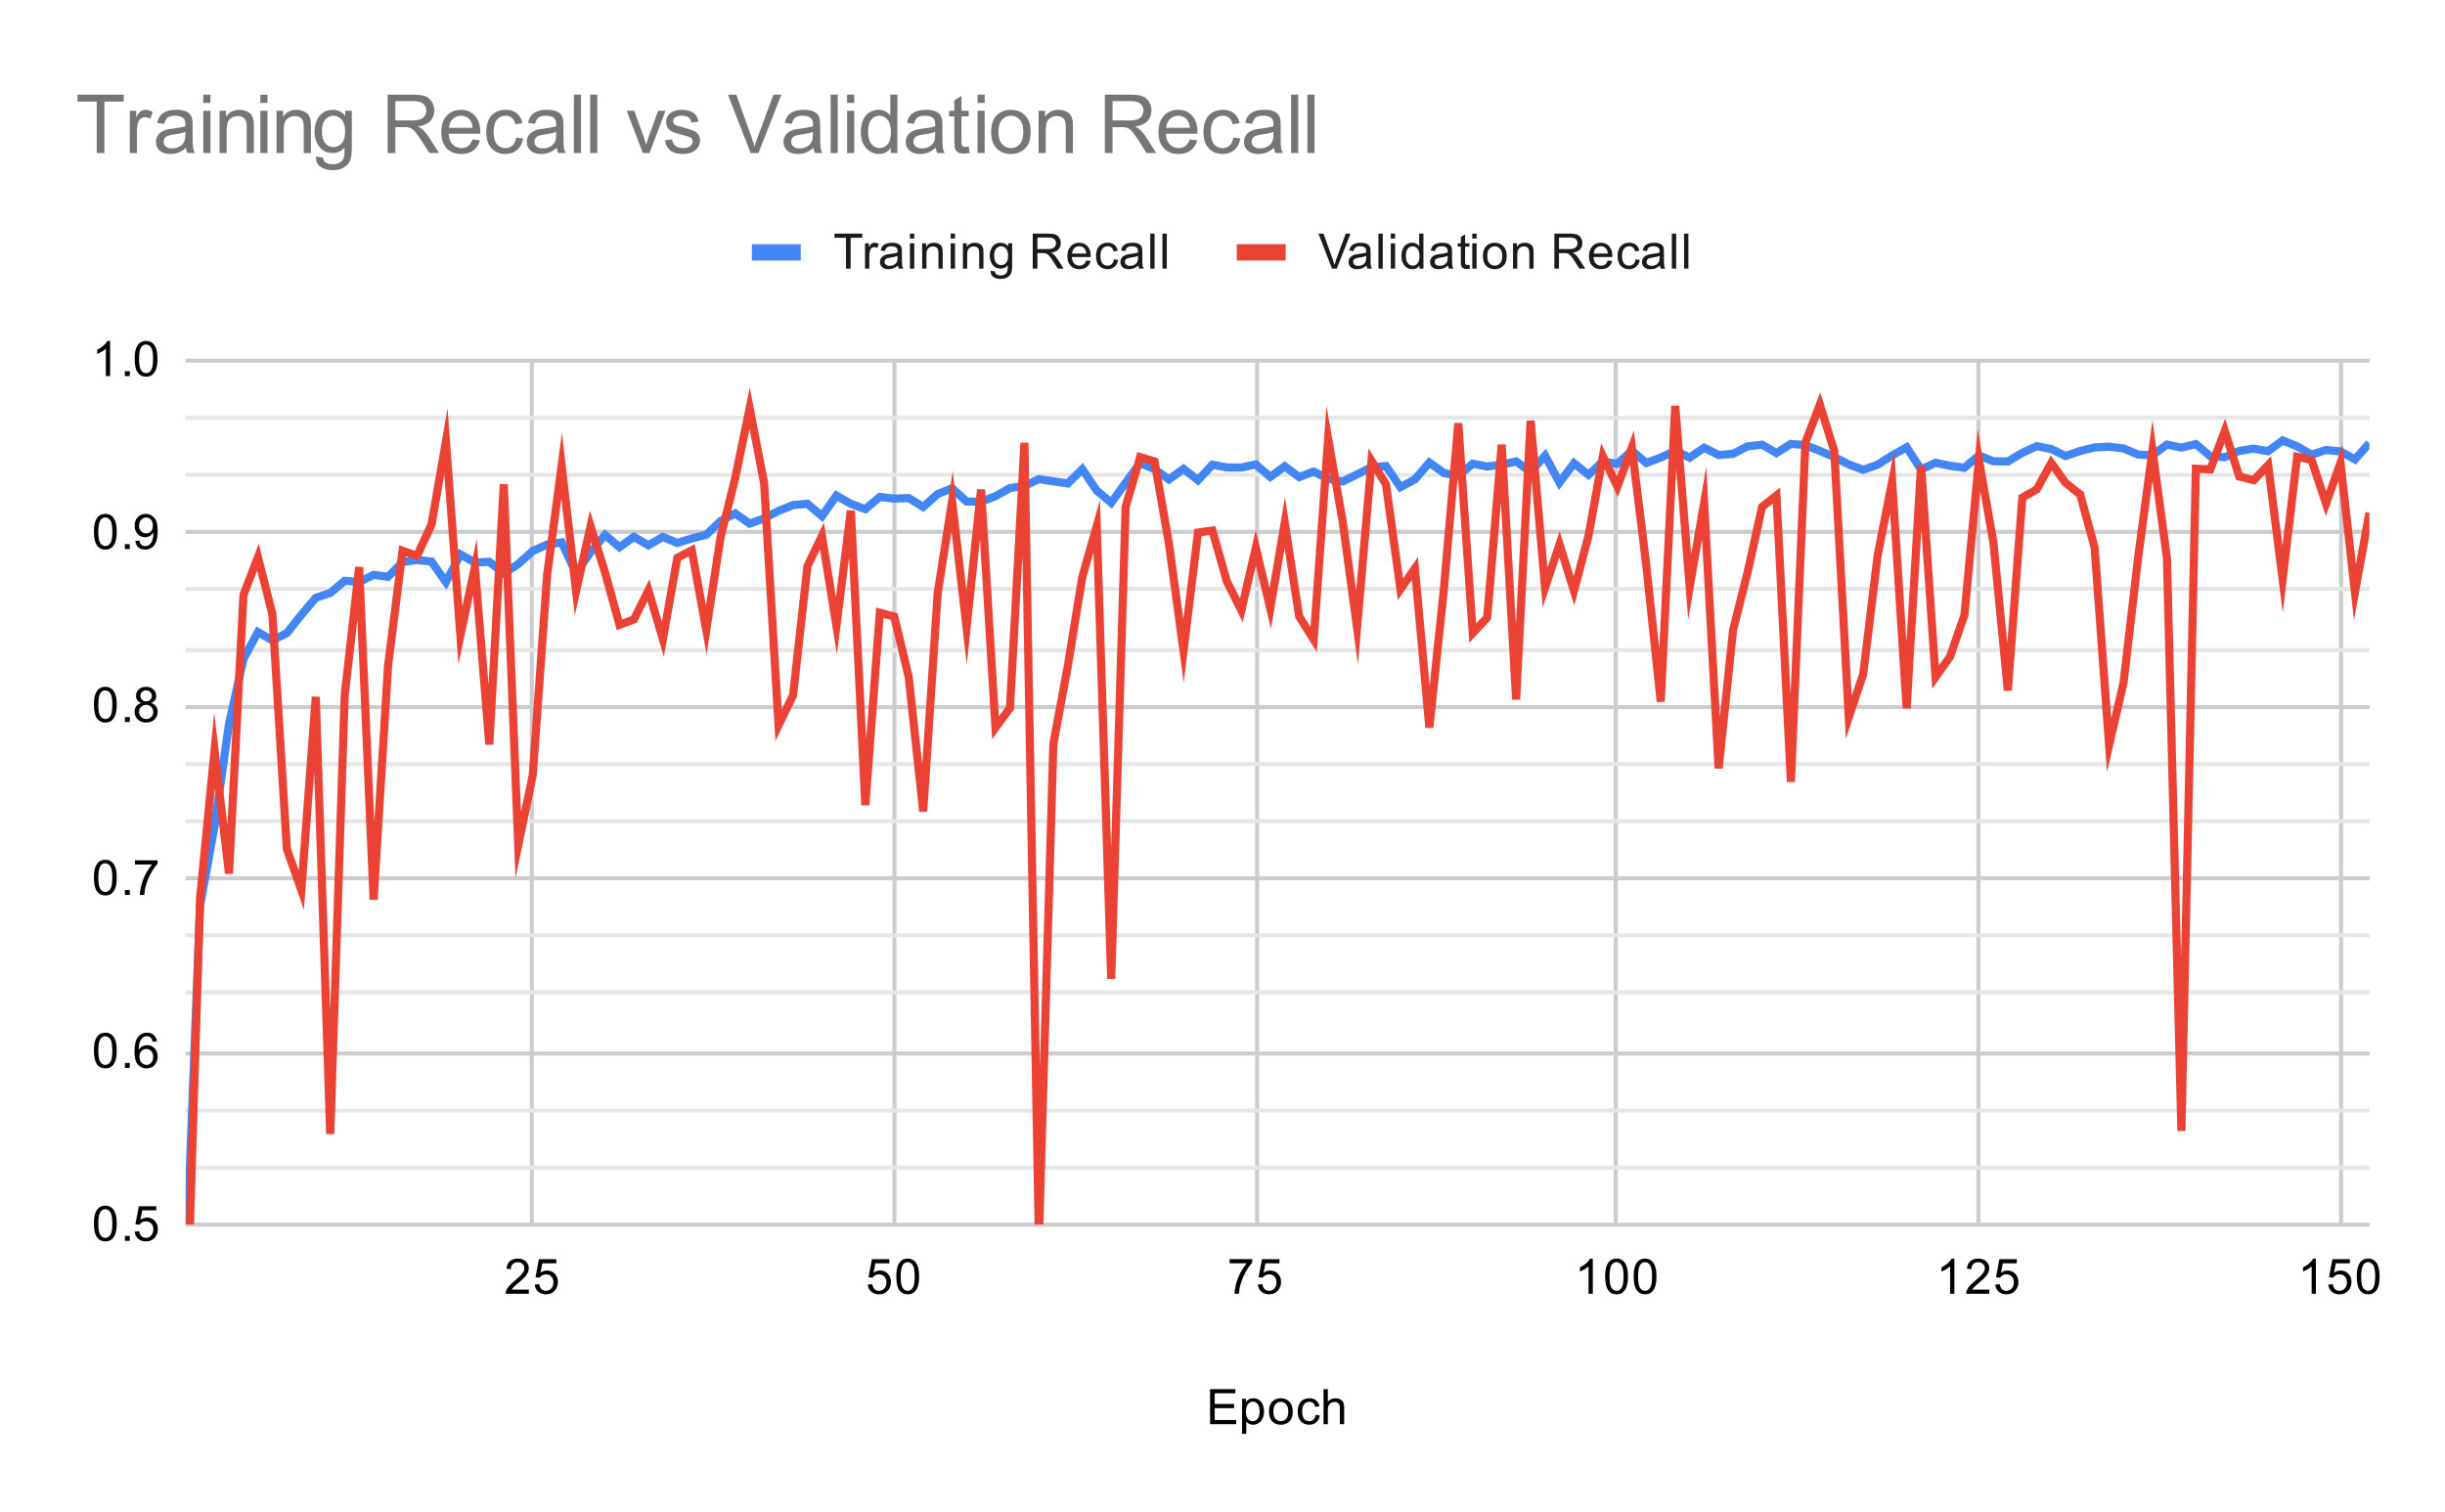
\includegraphics[width=0.3\textwidth]{figs/Project Charts/Training Recall vs Validation Recall.jpg} &
        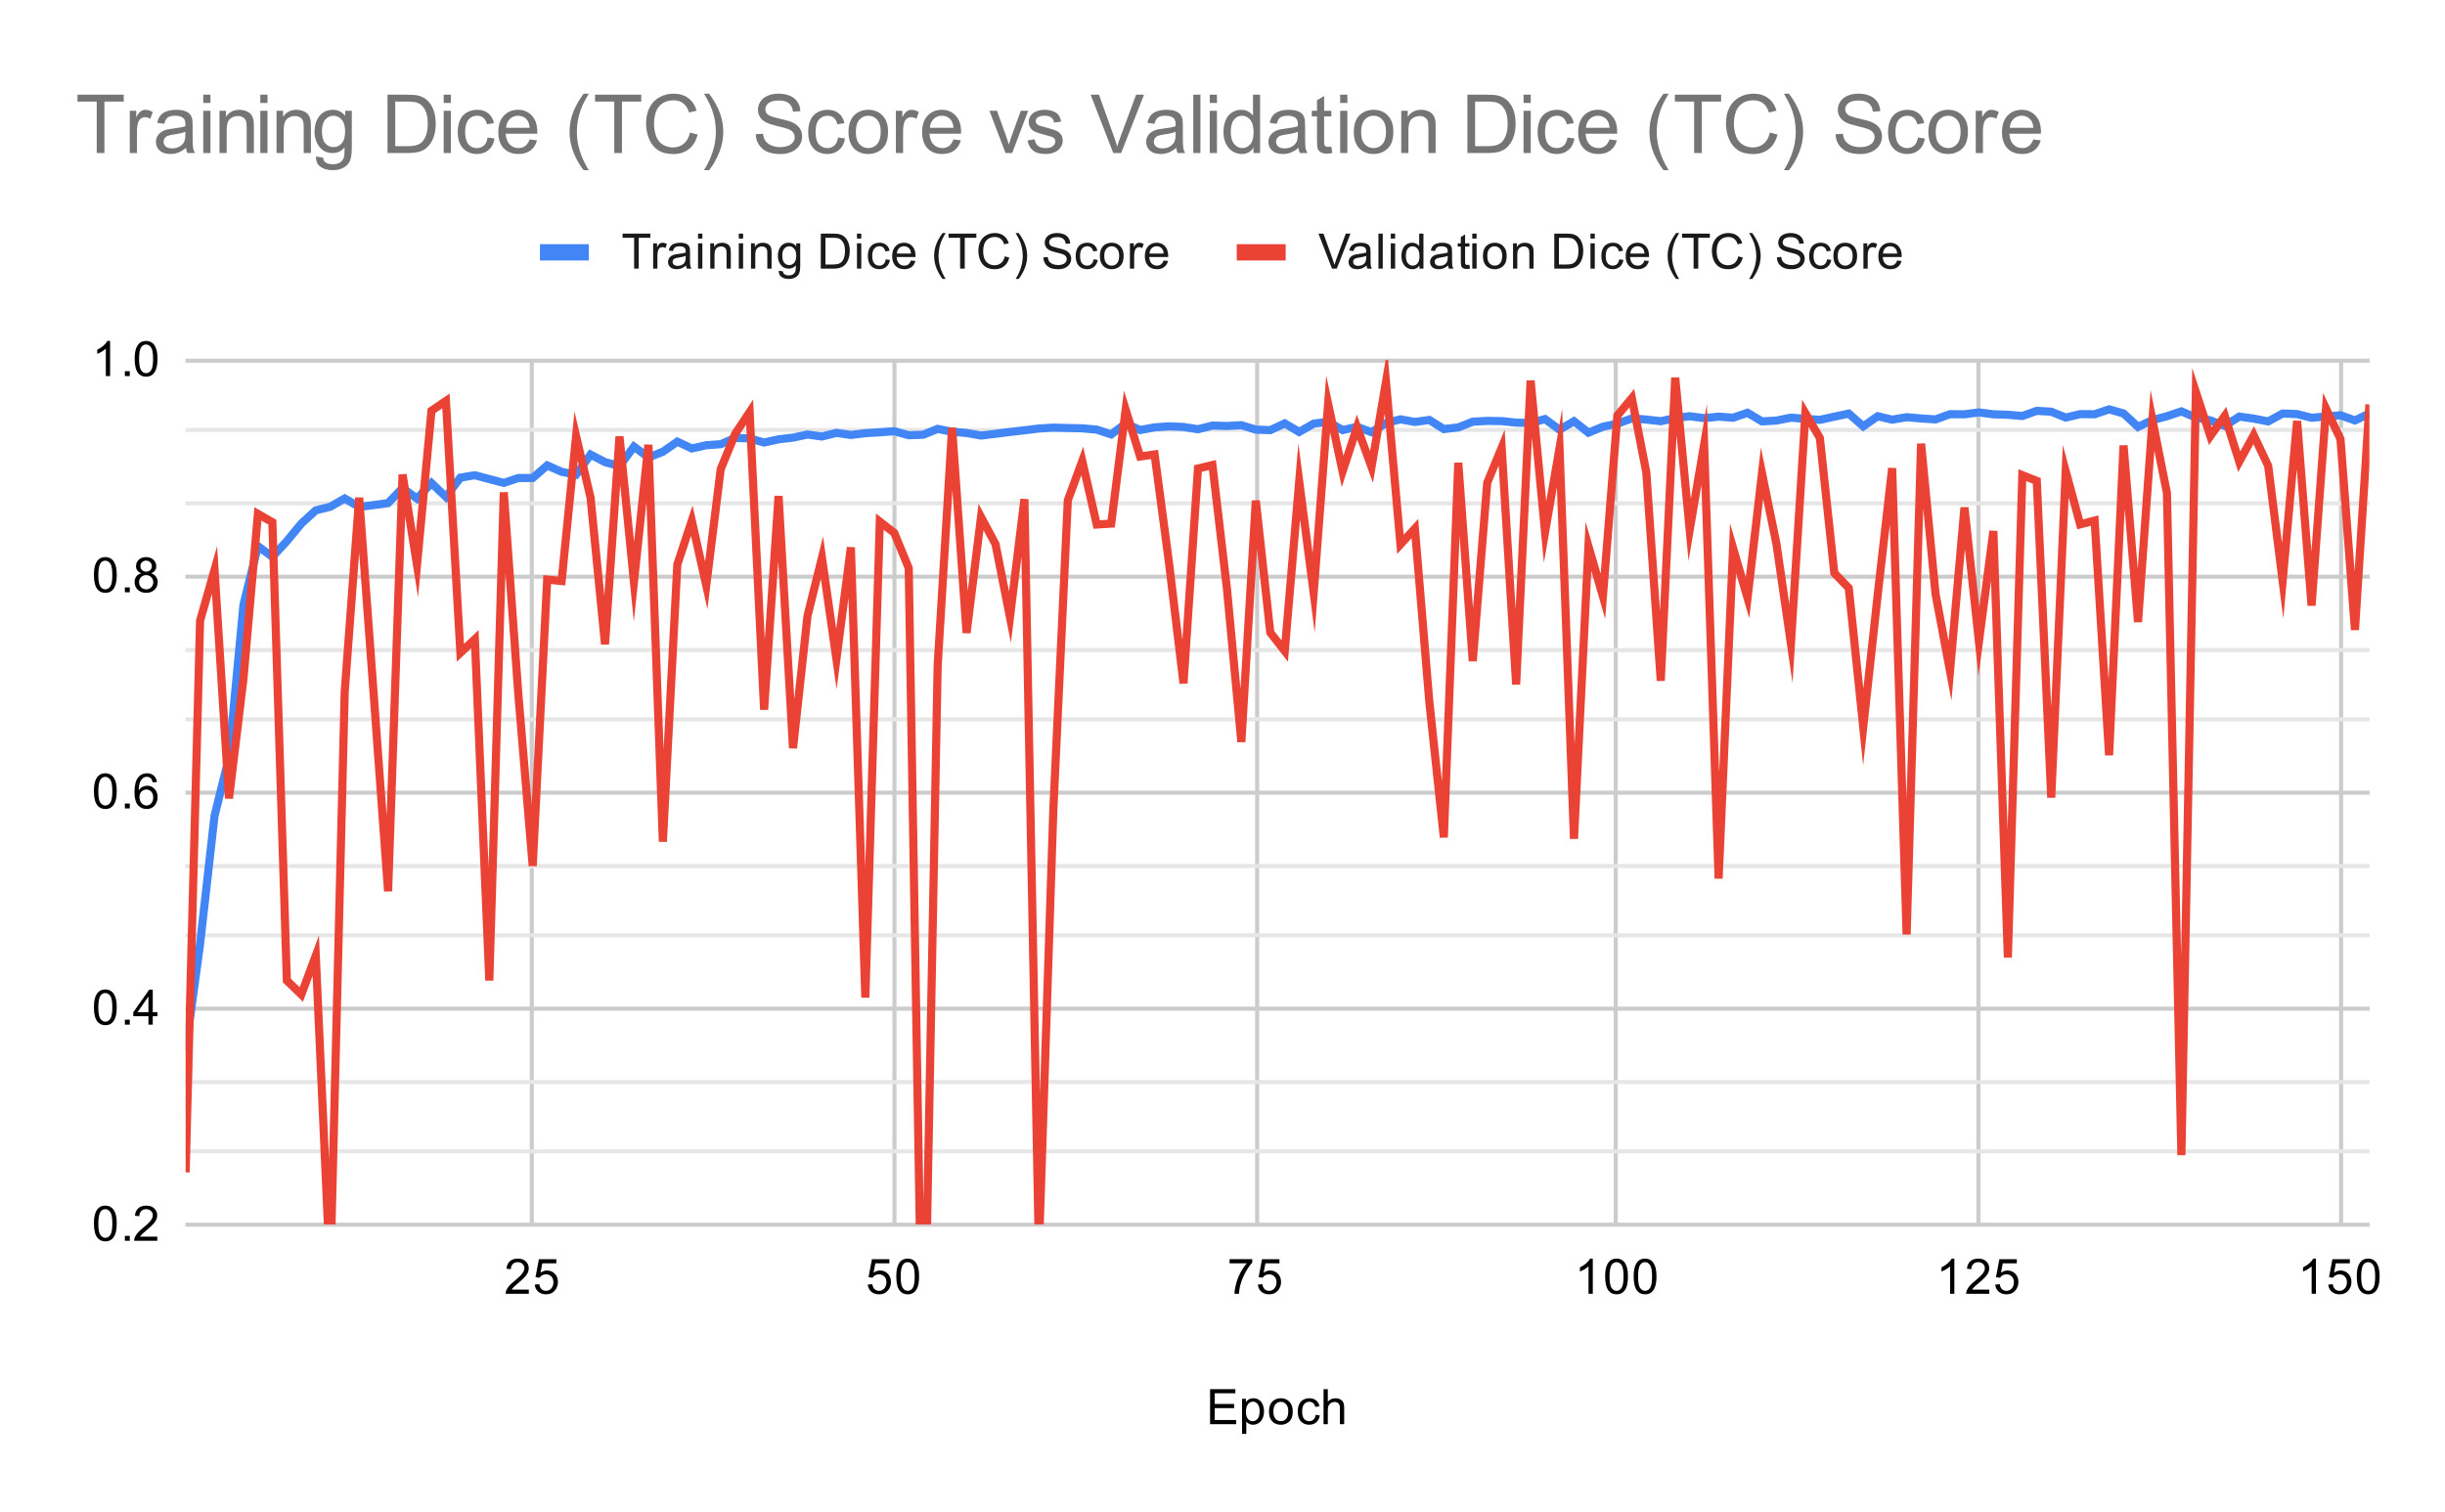
\includegraphics[width=0.3\textwidth]{figs/Project Charts/Training Dice (TC) Score vs Validation Dice (TC) Score.jpg} &
        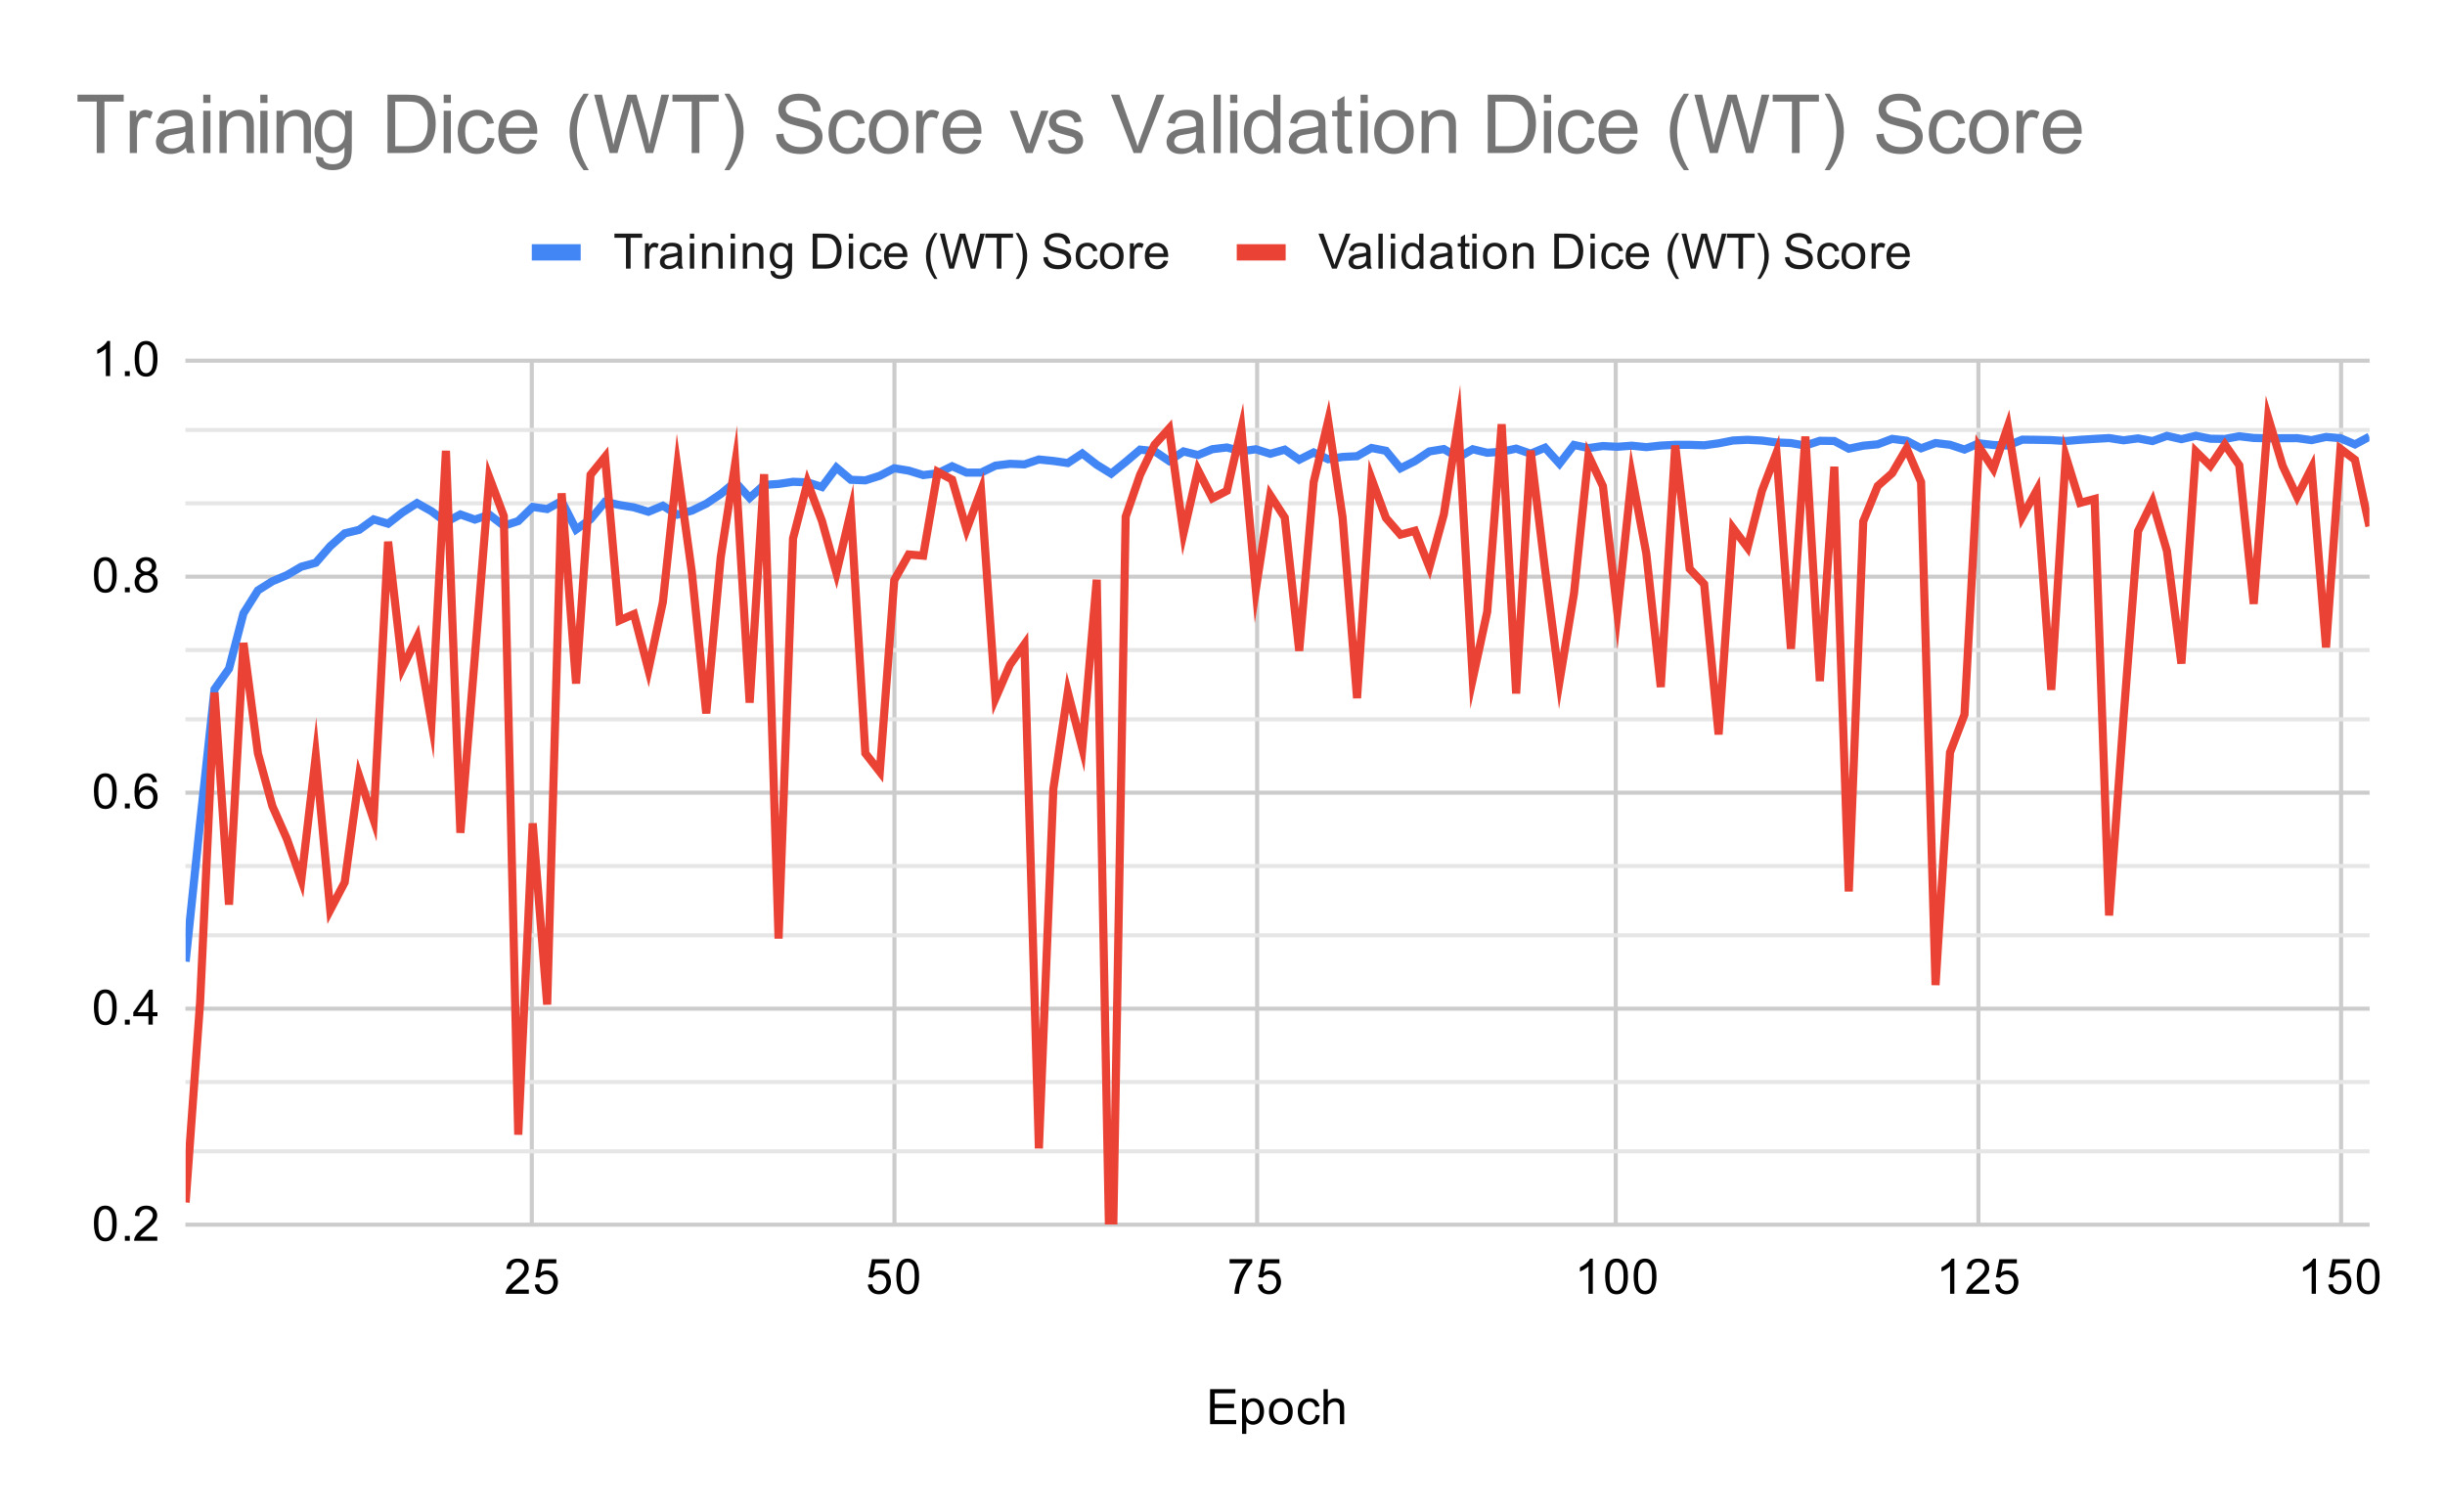
\includegraphics[width=0.3\textwidth]{figs/Project Charts/Training Dice (WT) Score vs Validation Dice (WT) Score.jpg} \\
        (g) Recall Graph & (h) TC Dice Score Graph & (i) WT Dice Score Graph \\[6pt]

        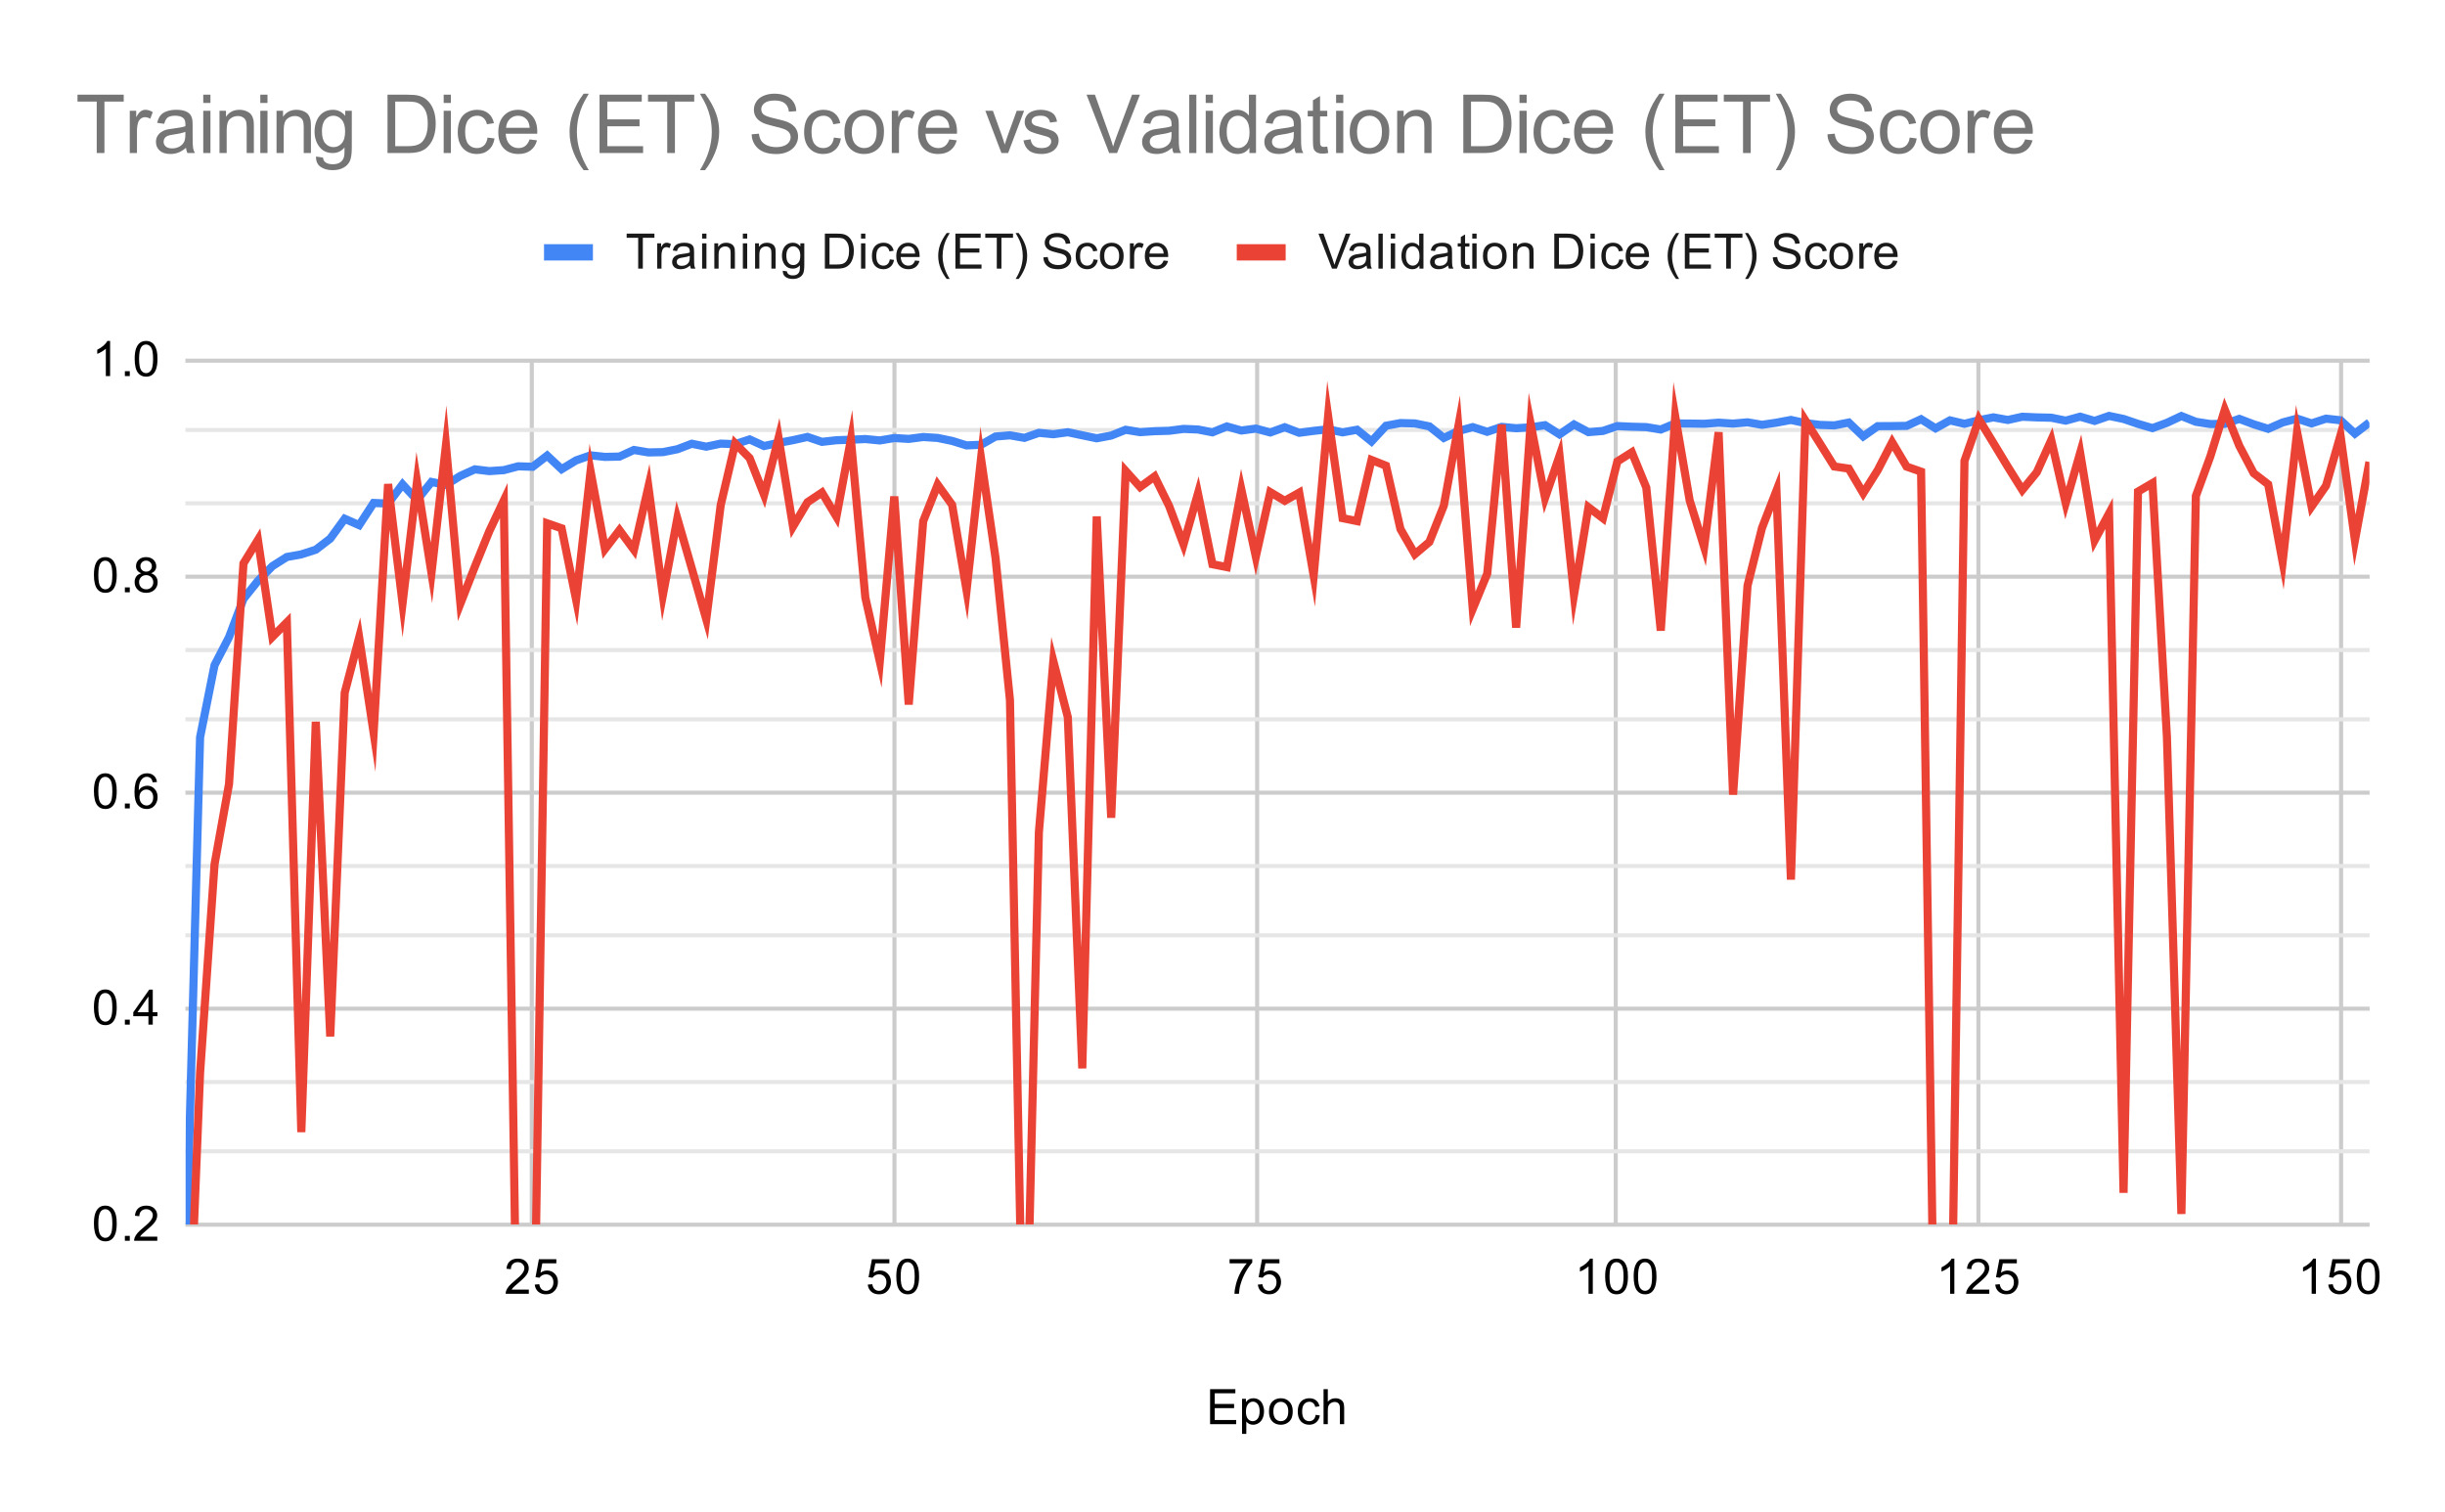
\includegraphics[width=0.3\textwidth]{figs/Project Charts/Training Dice (ET) Score vs Validation Dice (ET) Score.jpg} &
        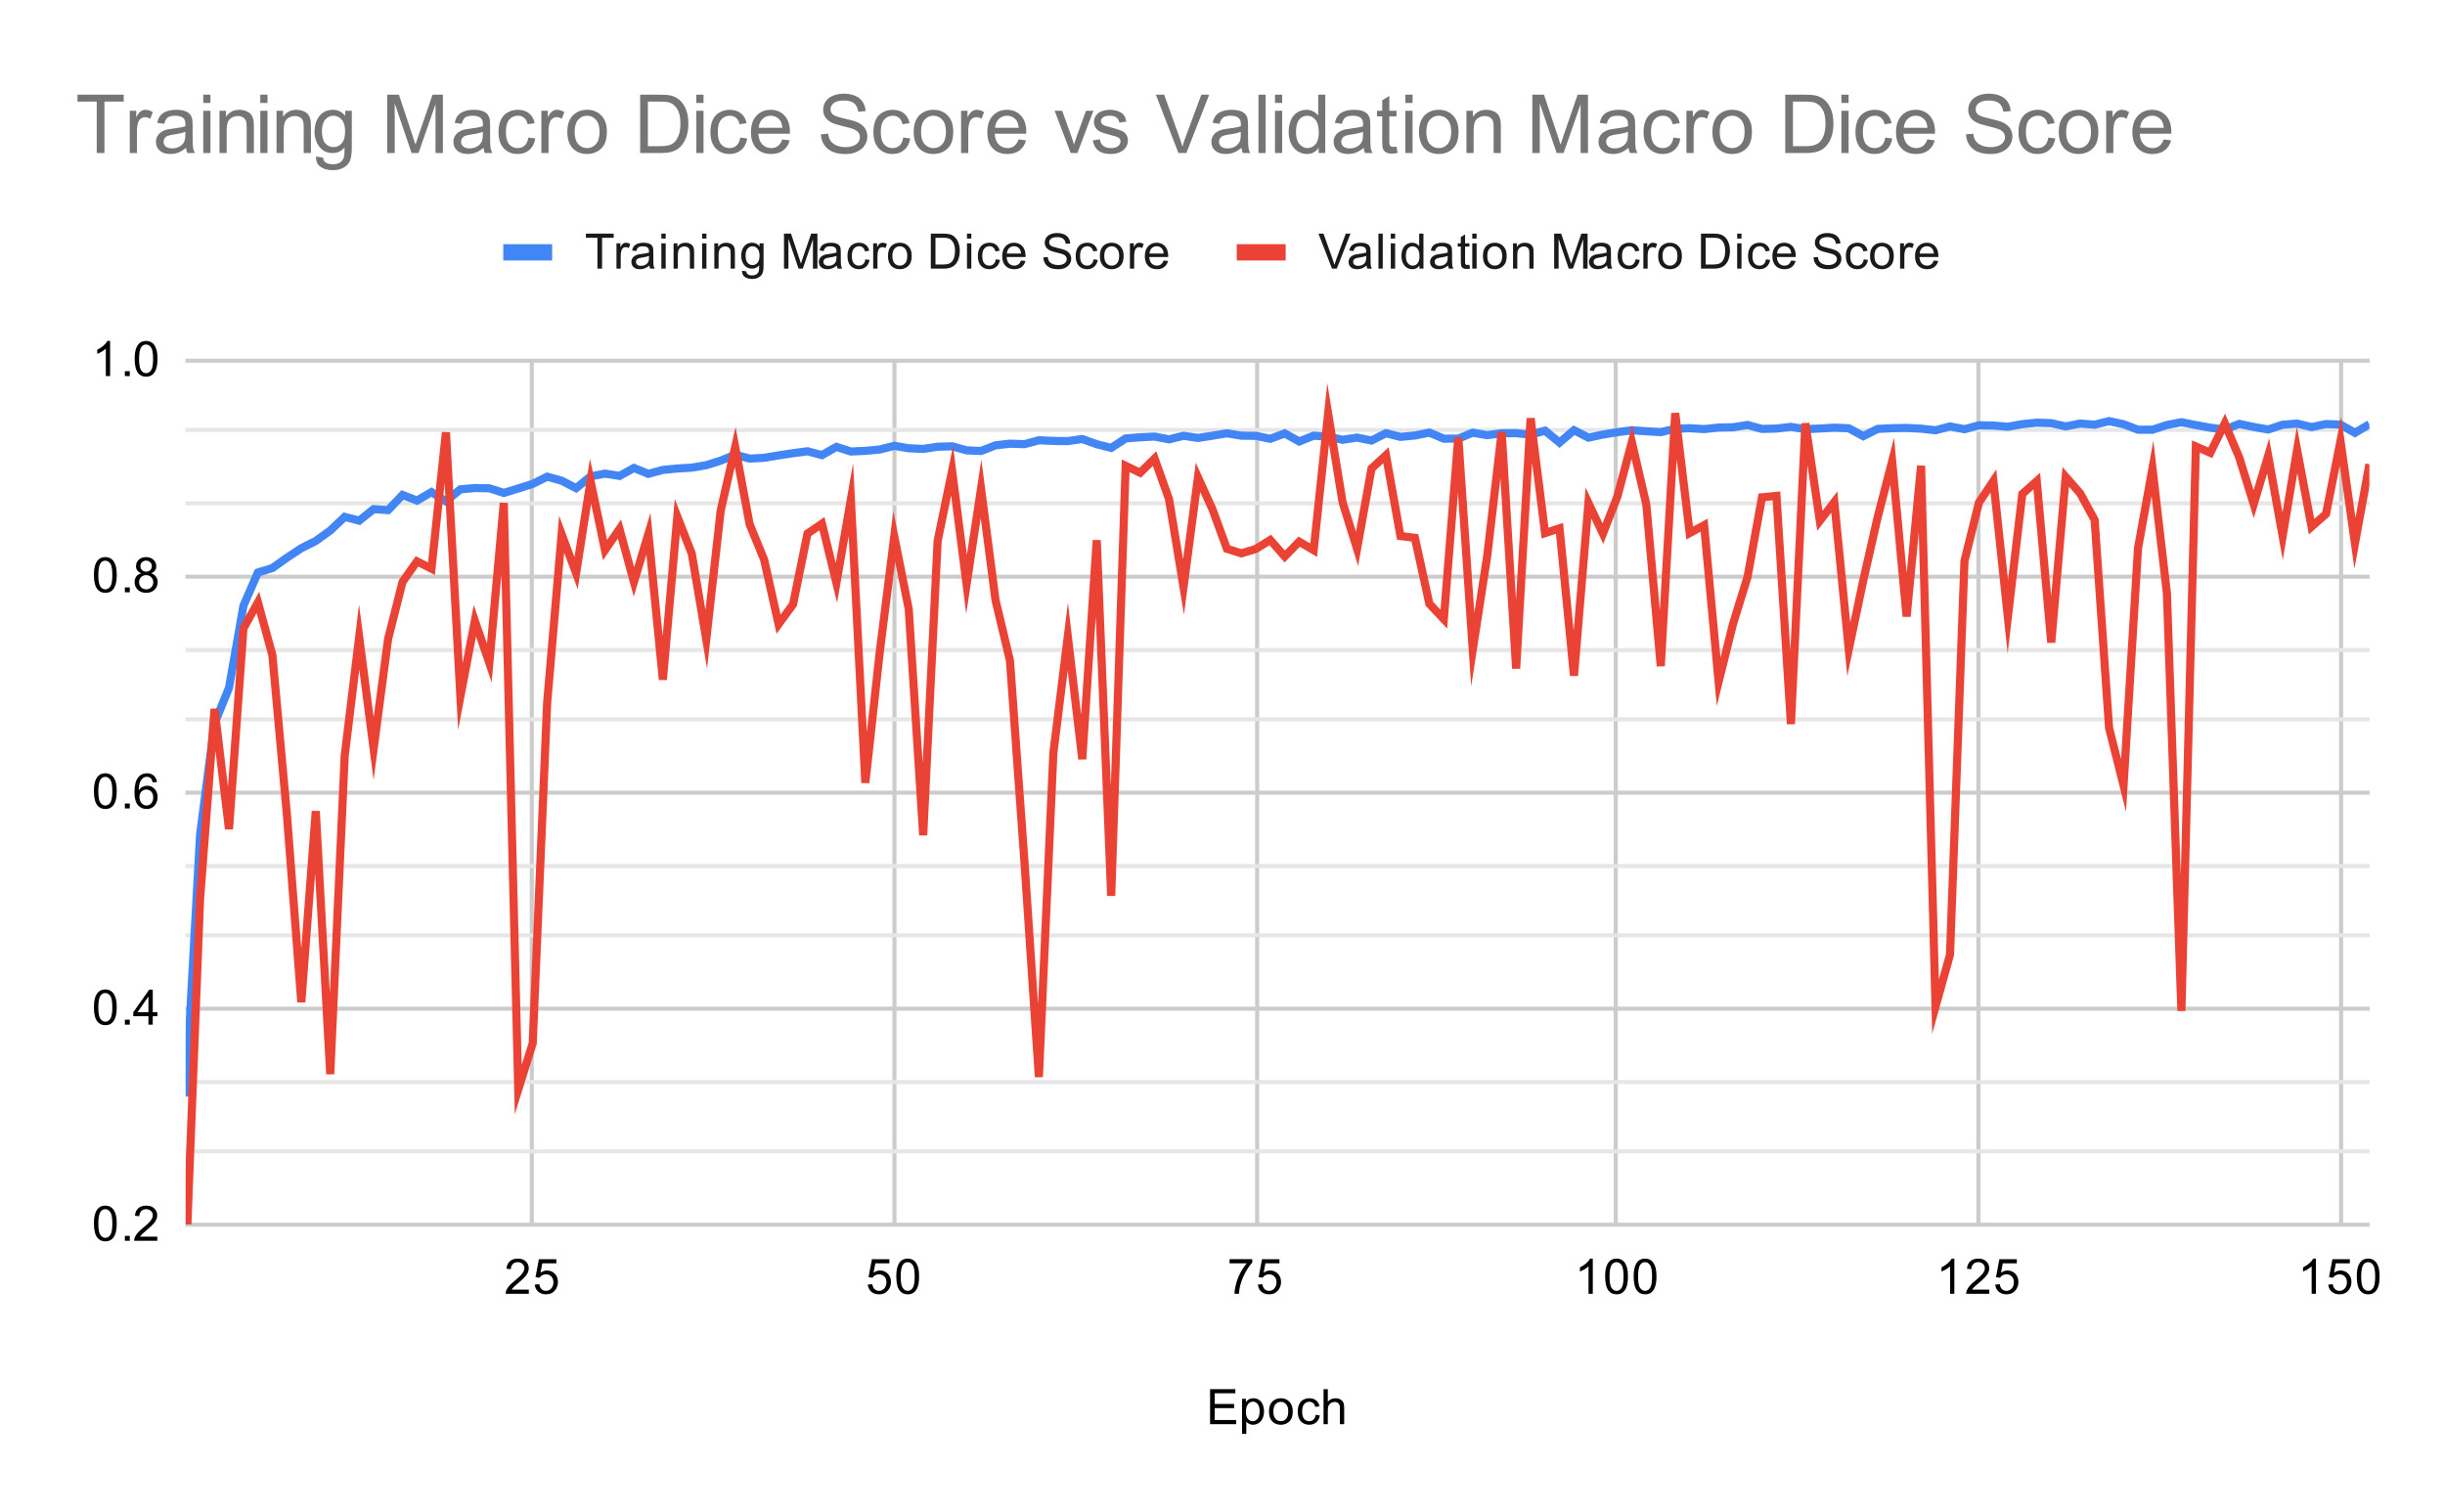
\includegraphics[width=0.3\textwidth]{figs/Project Charts/Training Macro Dice Score vs Validation Macro Dice Score.jpg} & \\
        (j) ET Dice Score Graph & (k) Macro Dice Score Graph &
    \end{tabular}
    \caption{Performance graphs across different evaluation metrics (Training represented as Blue and Validation represented as Red).}
    \label{fig:5x2_graphs}
\end{figure*}

\subsection{Quantitative and Qualitative Analysis}

We evaluated our proposed U-Net variant on the merged BraTS 2020 and 2021 training sets. A 75/25 split was applied, with 25\% of the cases held out for validation. Each case included four co-registered MRI modalities—T1, T1Gd (post-contrast), T2, and FLAIR—along with voxel-wise labels produced by expert neuro radiologists. Label definitions and pre-processing followed the BraTS challenge conventions.

Training continued up to epoch 152, with validation loss and segmentation metrics tracked throughout. We report both the best values observed during training and the final results at epoch 152. Best values reflect the model's peak capability, which could be recovered through checkpoint selection or ensembling.

The results in Table~\ref{tbl1} show balanced and strong performance across tumor subregions, with the highest stability for the Tumor Core (TC) and consistently solid scores for the Enhancing Tumor (ET). Dice WT showed a larger gap between the best and final, highlighting greater sensitivity to checkpoint selection and training dynamics. The best performance the model provides is for the TC region which confirms our proposed dense residual-inception blocks and attention modules are well capable of robust segmentation. The achieved dice score for ET and WT being 0.9055 and 0.8459 respectively and their peak being 0.9538 and 0.9466 shows that model is well capable of segmenting small and heterogeneous classes, but we need to be better at checkpoint selection rather than training the model for a set amount of epochs.

The graphical representations corresponding to each result are provided in Figure~\ref{fig:5x2_graphs} for clarity.

For qualitative assessment, representative segmentation results generated by the final trained model are presented in Figure~\ref{fig:5x2_graphs1}.

\begin{figure*}[!htbp]
    \centering
    \begin{tabular}{ccc}
        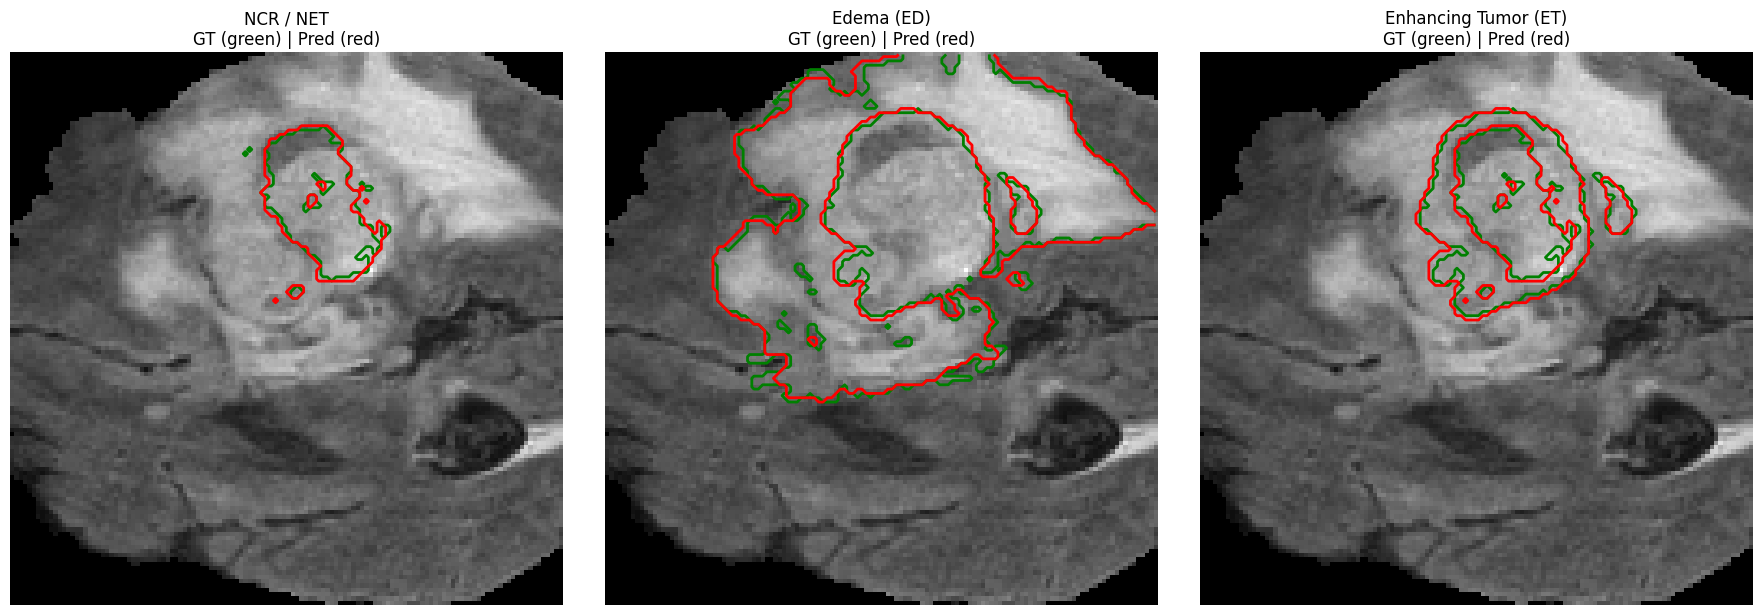
\includegraphics[width=0.31\textwidth]{figs/Conture of Tumor Over Flair images/Image 0.png} &
        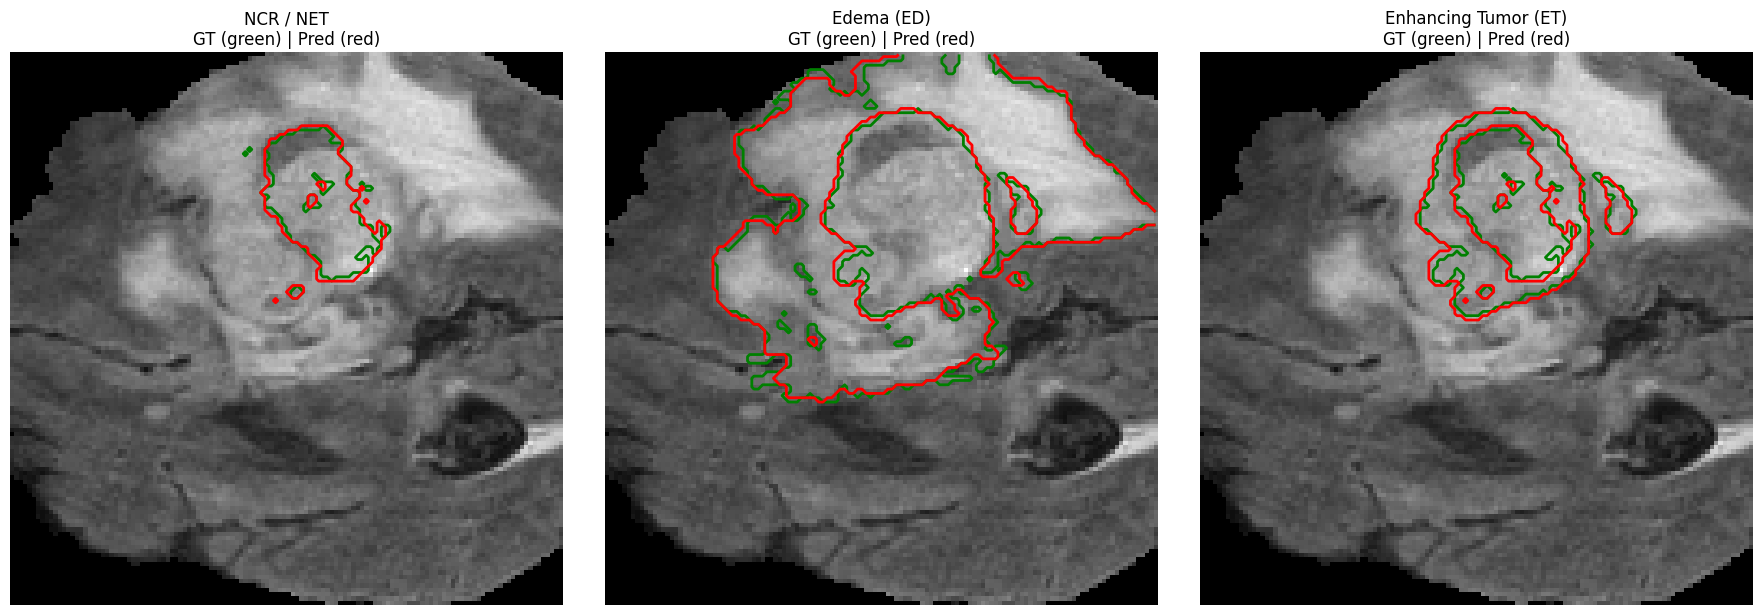
\includegraphics[width=0.31\textwidth]{figs/Conture of Tumor Over Flair images/Image 1.png} &
        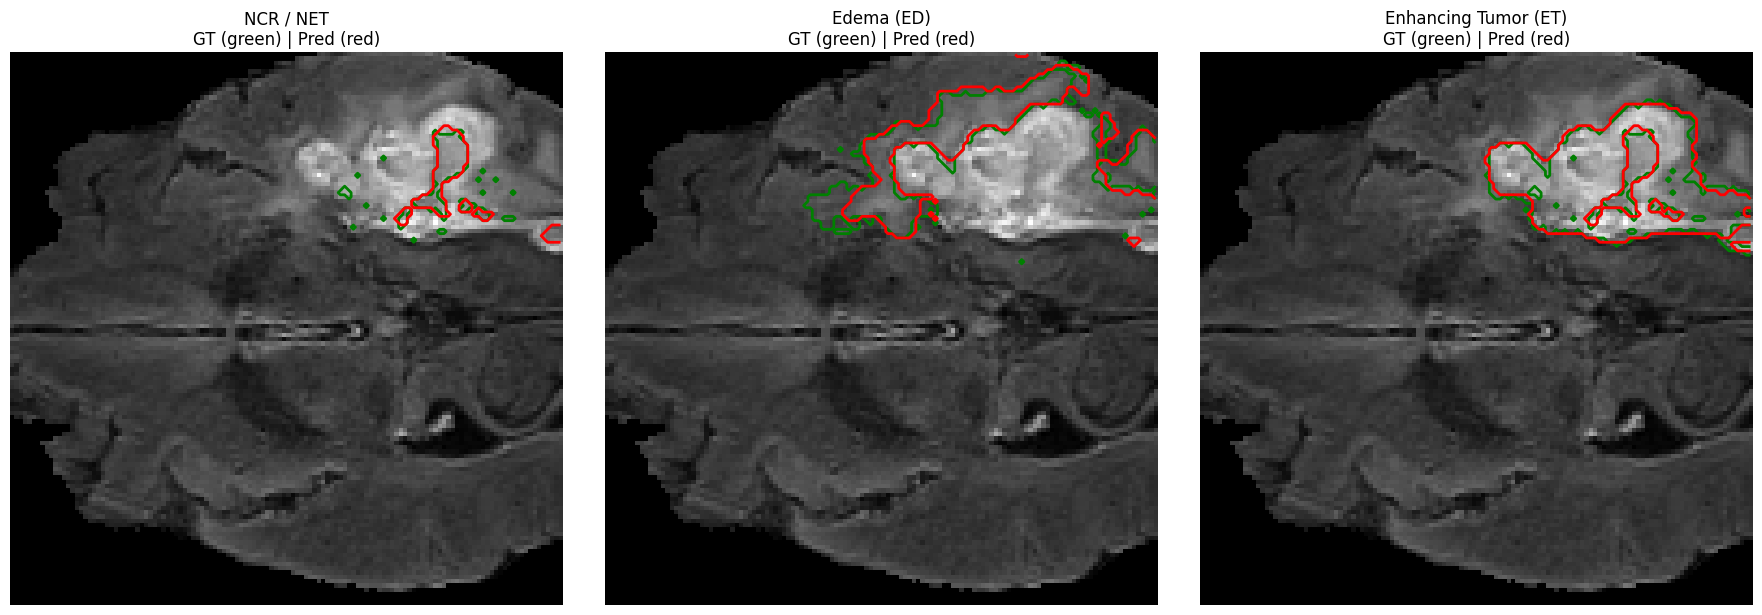
\includegraphics[width=0.31\textwidth]{figs/Conture of Tumor Over Flair images/Image 28.png} \\
        Example 1 & Example 2 & Example 3 \\

        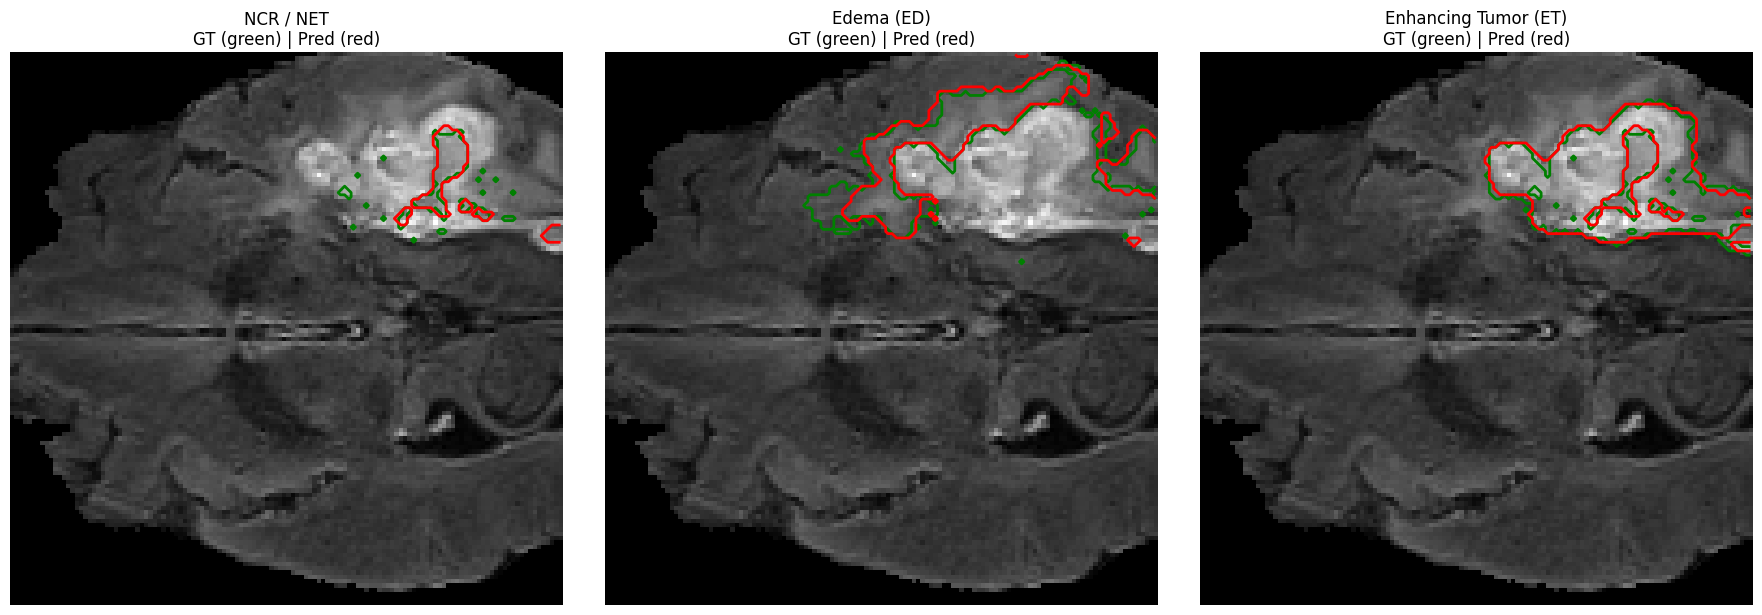
\includegraphics[width=0.31\textwidth]{figs/Conture of Tumor Over Flair images/Image 53.png} &
        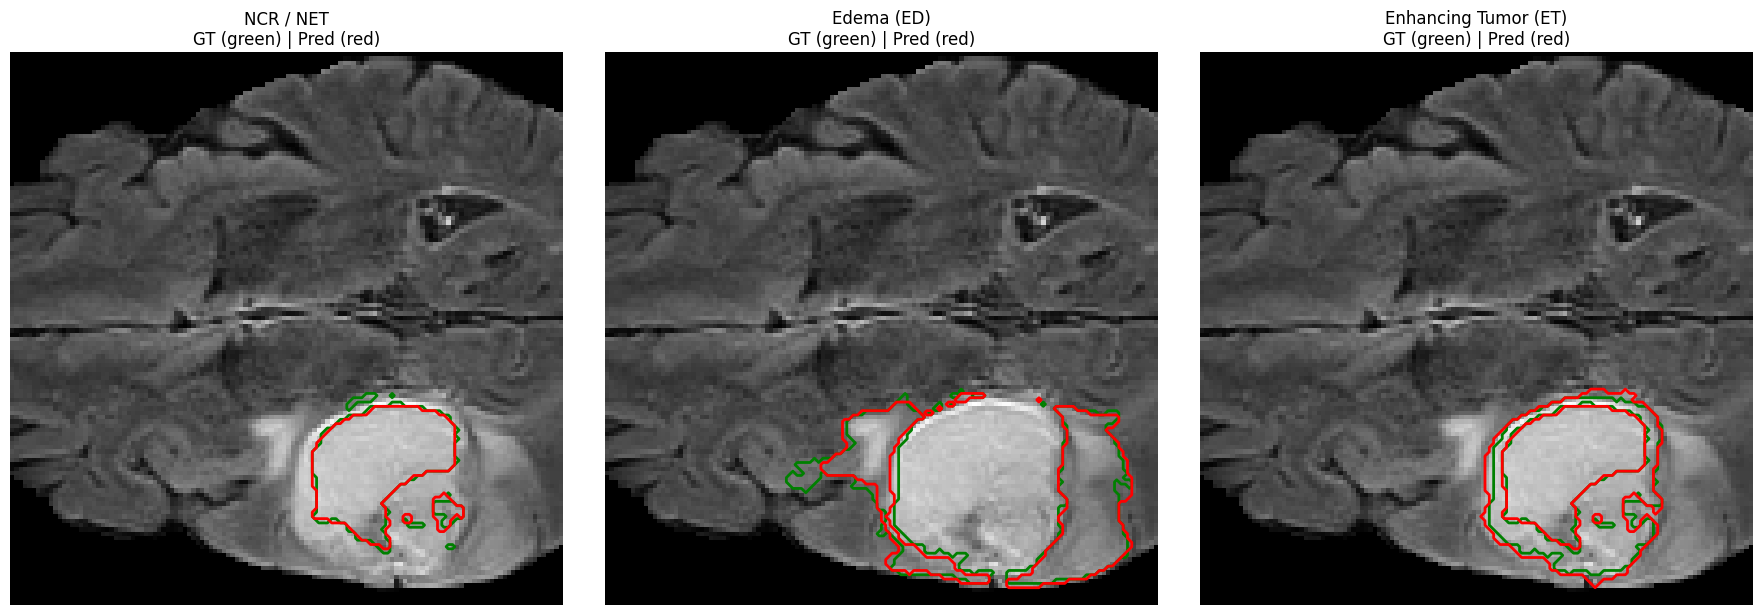
\includegraphics[width=0.31\textwidth]{figs/Conture of Tumor Over Flair images/Image 57.png} &
        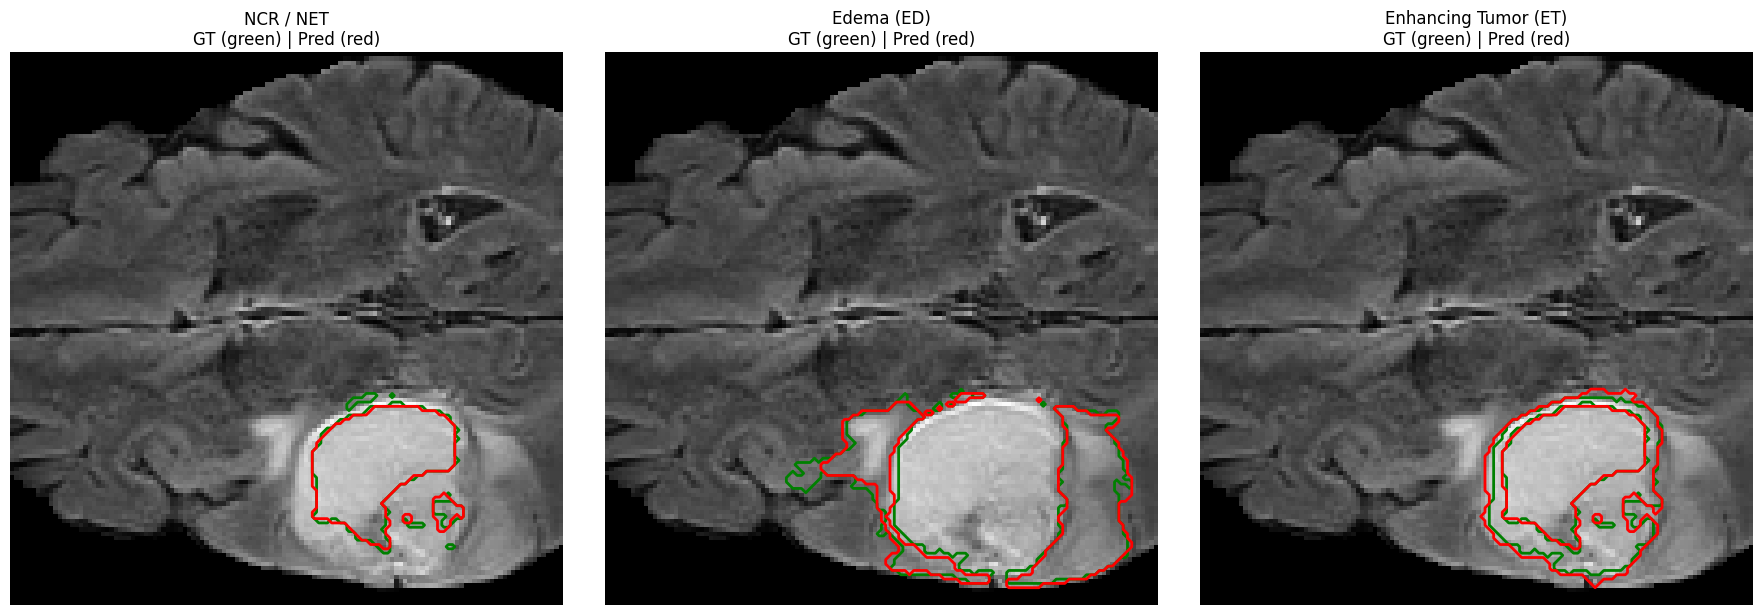
\includegraphics[width=0.31\textwidth]{figs/Conture of Tumor Over Flair images/Image 59.png} \\
        Example 4 & Example 5 & Example 6 \\

        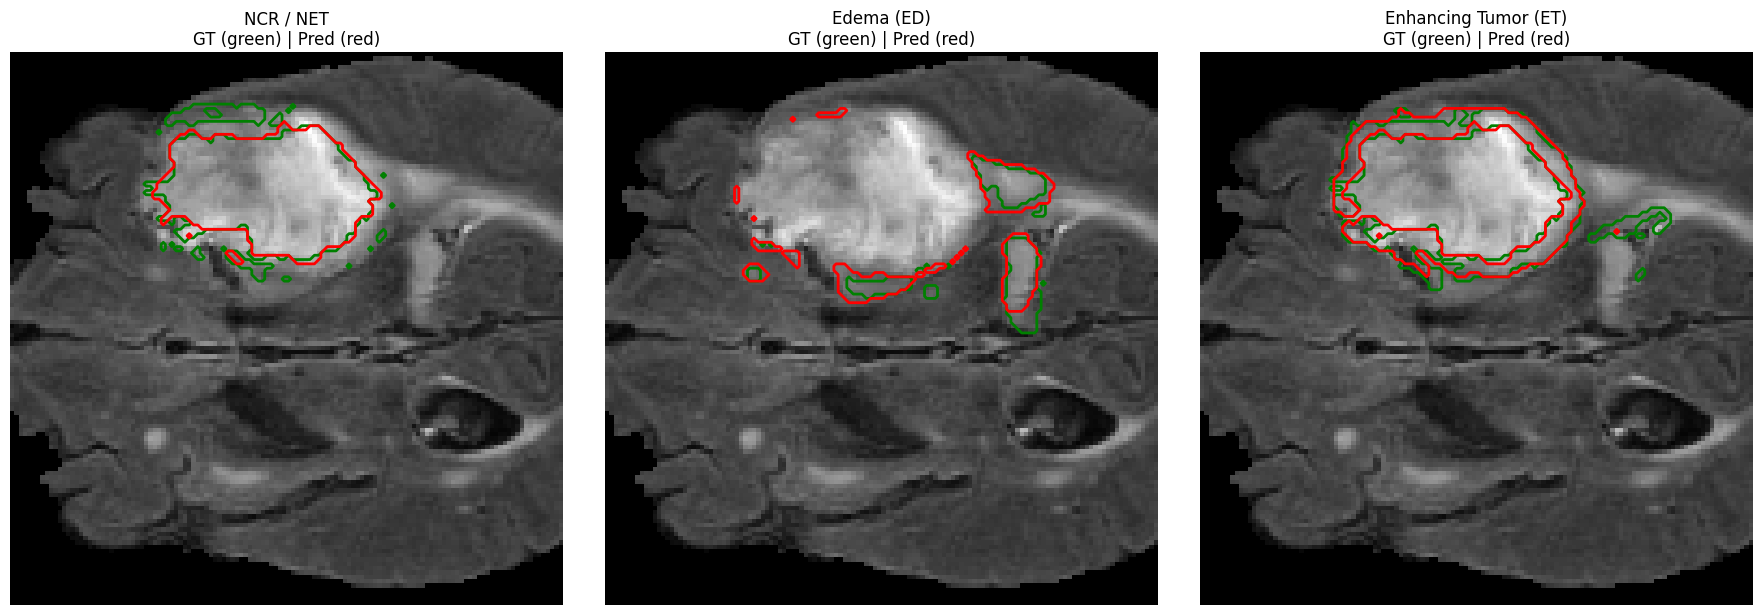
\includegraphics[width=0.31\textwidth]{figs/Conture of Tumor Over Flair images/Image 63.png} &
        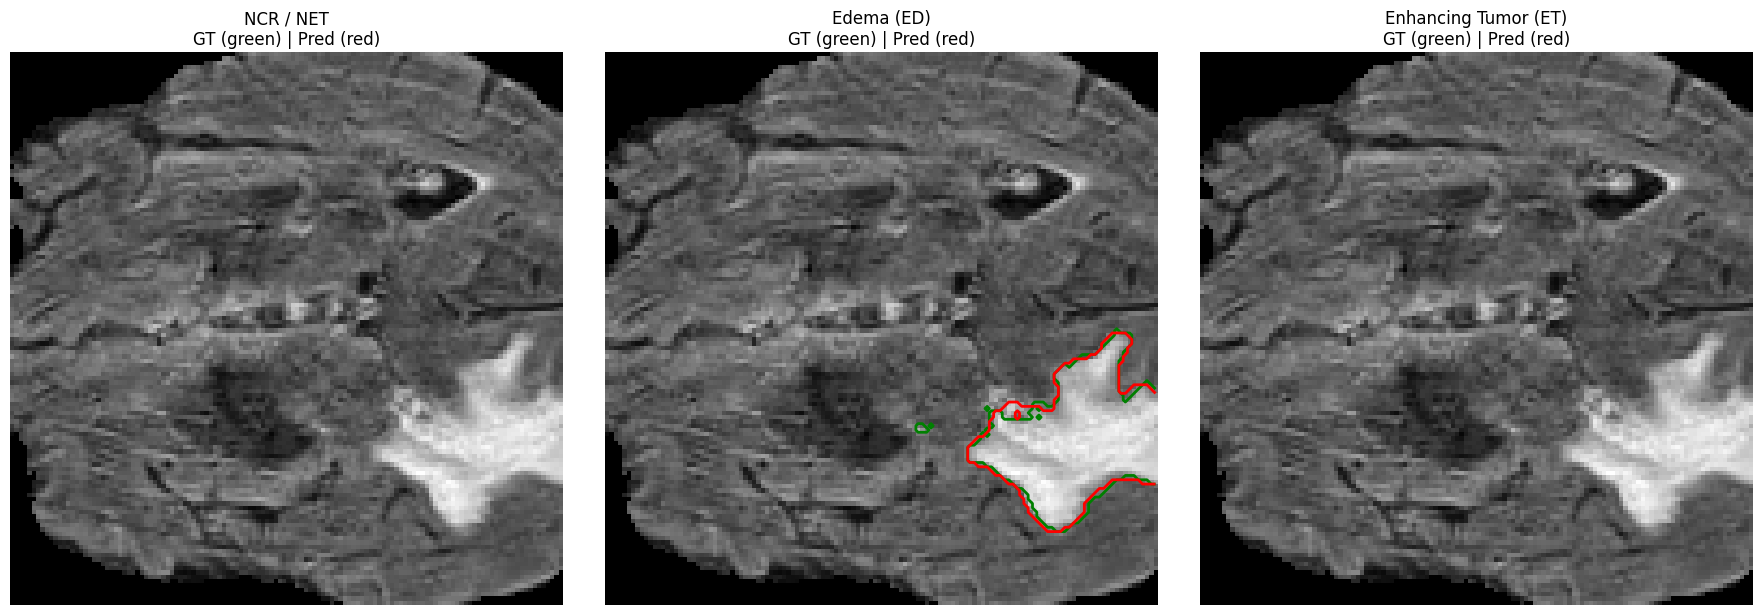
\includegraphics[width=0.31\textwidth]{figs/Conture of Tumor Over Flair images/Image 66.png} &
        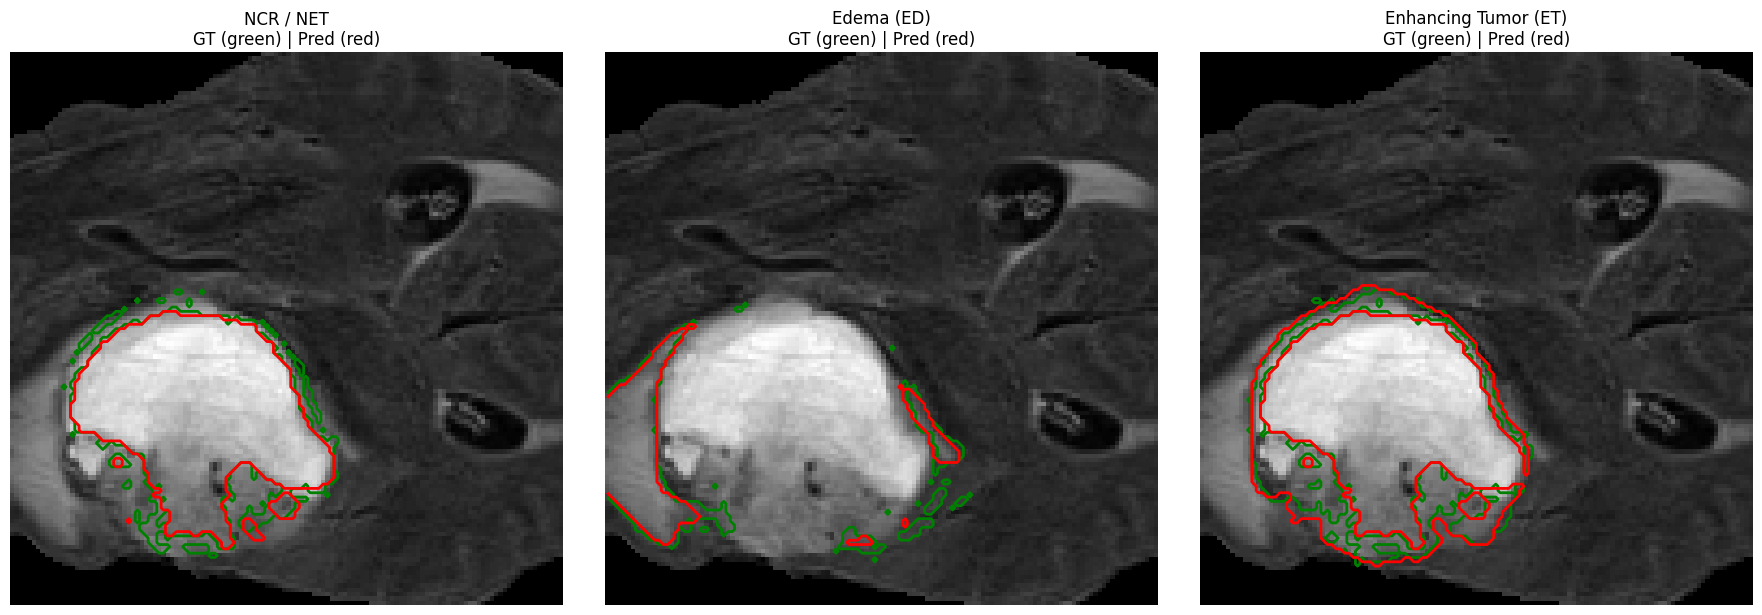
\includegraphics[width=0.31\textwidth]{figs/Conture of Tumor Over Flair images/Image 74.png} \\
        Example 7 & Example 8 & Example 9\\
    \end{tabular}
    \caption{Ground Truth region Conture vs Predicted region Conture for different channels (Ground Truth Represented as Green and Prediction Represented as Red)}
    \label{fig:5x2_graphs1}
\end{figure*}

\subsection{Robustness}

The proposed model is evaluated against other popular network architectures to assess its performance. The comparative results, in Table \ref{tab:brats_comparison}, demonstrate the effectiveness and robustness of the proposed method.

\begin{table*}[!htbp]
    \caption{Comparison of Dice scores on BraTS benchmark datasets.}
    \label{tab:brats_comparison}
    \centering
    \begin{tabular}{lcccc}
        \toprule
        Model (Dataset / Year) & WT Dice & TC Dice & ET Dice & Source \\
        \midrule
        Myronenko (BraTS 2018)                    & 0.884 & 0.815 & 0.766 & BraTS 2018 Test \\
        Two-Stage Cascaded U-Net (BraTS 2019)      & 0.888 & 0.837 & 0.833 & BraTS 2019 Test \\
        nnU-Net (BraTS 2020)                       & 0.890 & 0.851 & 0.820 & BraTS 2020 Test \\
        TransBTS (2021)                            & 0.900 & 0.819 & 0.789 & Reported (TTA)  \\
        Swin UNETR (2022)                          & 0.926 & 0.885 & 0.858 & Validation      \\
        SwinBTS (2022)                             & 0.918 & 0.848 & 0.832 & Reported        \\
        BiTr-UNet (BraTS 2021)                     & 0.926 & 0.935 & 0.887 & BraTS 2021 Test \\
        Triplanar Ensemble (BraTS 2020)            & 0.890 & 0.840 & 0.810 & BraTS 2020 Test \\
        S3D-UNet (2018)                            & 0.839 & 0.783 & 0.689 & Reported        \\
        Cascaded V-Nets (BraTS 2018)               & 0.876 & 0.795 & 0.736 & BraTS 2018 Test \\
        \textbf{Our Model (BraTS 2020+2021)}       & \textbf{0.846} & \textbf{0.959} & \textbf{0.906} & 75/25 Validation \\
        \bottomrule
    \end{tabular}
\end{table*}

On validation, our model ranks among top performers for TC and ET, with Dice scores of $0.959$ and $0.906$ respectively. While WT Dice was $0.846$ at the final epoch—slightly lower than models reporting >0.90—our peak WT Dice reached $0.947$, indicating checkpointing or ensembling could close this gap. Overall, the model delivers competitive performance, particularly for TC and ET segmentation, aligning with recent transformer-hybrid models.

\subsection{Computational Complexity}

One notable advantage of the proposed model is its computational efficiency is that it being light-weight. When we compare the parameter count of our model with others we observe the following in Table \ref{tab:parameter_comparison}.

\begin{table*}[!htbp]
    \caption{Comparison of total trainable parameters across recent 3D segmentation models.}
    \label{tab:parameter_comparison}
    \centering
    \begin{tabular}{lcc}
        \toprule
        Model (Ref.)                           & Total Parameters (M) & Remarks \\
        \midrule
        \textbf{Our Model (this work)}         & \textbf{4.01} & All parameters trainable  \\
        SegFormer3D (2024)                     & 4.50          & Lightweight transformer   \\
        LightM-UNet                            & 5.02          & Lightweight baseline      \\
        3D U-Net                               & 16.21         & Canonical 3D configuration \\
        VT-UNet-B                              & 20.80         & Transformer-based encoder \\
        TransBTS (2021)                        & 32.99         & CNN + Transformer hybrid  \\
        nnU-Net (default)                      & $\sim$30.00   & Dataset-dependent configuration \\
        nnFormer                               & 39.70         & Hierarchical transformer  \\
        Swin UNETR (2022)                      & 61.98         & Swin transformer hybrid   \\
        UNETR (2021)                           & 102.50        & ViT-based encoder         \\
        \bottomrule
    \end{tabular}
\end{table*}

As shown in Table~\ref{tab:parameter_comparison}, the proposed model (4.01M parameters) is substantially lighter than transformer-based architectures such as Swin UNETR (61.98M) and UNETR (102.5M). The proposed architecture achieves competitive segmentation performance while maintaining significantly lower computational complexity compared to contemporary transformer-based methods.

The proposed model can be categorized among lightweight segmentation architectures. Even if we compare the FLOPs~count of our model with others we get the following in Table~\ref{tab:complexity}.

\begin{table*}[!htbp]
    \caption{Comparison of model complexity in terms of trainable parameters and FLOPs.}
    \label{tab:complexity}
    \centering
    \begin{tabular}{lcc}
        \toprule
        Methods         & Parameters (M) & FLOPs (G) \\
        \midrule
        3D U-Net        & 7.74   & 586.71  \\
        Attention U-Net & 17.12  & 588.26  \\
        VNet            & 7.03   & 769.30  \\
        Swin-Unet       & 27.15  & 250.88  \\
        HDC-Net         & 0.29   & 25.62   \\
        TransUNet       & 105.18 & 1205.76 \\
        TransBTS        & 30.61  & 263.82  \\
        MCSLF-Net       & 24.49  & 142.43  \\
        \bottomrule
    \end{tabular}
\end{table*}

Reported as per Mingzhe Zhou et al., we can see this model might not rank among the Ultra-Lightweight models like HDC-Net. But we can comfortably place it in the category of light weight model.


%% ============================================================
%% SECTION: Conclusion
%% ============================================================

\section{Conclusion}

This proposed model performs on par with, and in some cases exceeds, established image segmentation architectures, managing to compete with popular Transformer based networks, while being much lightweight than most of them. In this paper, we have not shown justifications for many of the improvements that we have made. For example we have not shown any evidence that our adaptive loss function works better than other mainstream loss functions like Tversky or Boundary loss; or even if it works better than Dice Loss or Categorical Focal Loss stand alone. Also in case of our DRIC block, we have not formally tested if all components of that block is strictly necessary, or how it performs compared to already available/popular Dense, Residual, or Inception block. These components of  the architecture have been decided by theoretical understanding and preliminary small-scale testing. We have failed to show any justification for them, mostly due to a lack of equipment and a lack of scope. Also we have not tested other criteria that could theoretically have boosted our model performance; for example other validation strategies like cross-validation or hold-out, data augmentation strategies, Other normalization approach, etc. We intend to test experiment with them in future expansion of the work, if the scope permits.

%There are various bibliography styles available. You can select the
%style of your choice in the preamble of this document. These styles are
%Elsevier styles based on standard styles like Harvard and Vancouver.
%Please use Bib\TeX\ to generate your bibliography and include DOIs
%whenever available.

%Here are two sample references:
%\cite{Fortunato2010}
%\cite{Fortunato2010,NewmanGirvan2004}
%\cite{Fortunato2010,Vehlowetal2013}

% \section{Floats}
% {Figures} may be included using the command,\linebreak
% \verb+\includegraphics+ in
% combination with or without its several options to further control
% graphic. \verb+\includegraphics+ is provided by {graphic[s,x].sty}
% which is part of any standard \LaTeX{} distribution.
% {graphicx.sty} is loaded by default. \LaTeX{} accepts figures in
% the postscript format while pdf\LaTeX{} accepts {*.pdf},
% {*.mps} (metapost), {*.jpg} and {*.png} formats.
% pdf\LaTeX{} does not accept graphic files in the postscript format.

% \begin{figure}
% 	\centering
% 		
\includegraphics[scale=.75]{figs/Fig1.pdf}
% 	\caption{The evanescent light - $1S$ quadrupole coupling
% 	($g_{1,l}$) scaled to the bulk exciton-photon coupling
% 	($g_{1,2}$). The size parameter $kr_{0}$ is denoted as $x$ and
% 	the \PMS is placed directly on the cuprous oxide sample ($\delta
% 	r=0$, See also Table \protect\ref{tbl1}).}
% 	\label{FIG:1}
% \end{figure}

% The \verb+table+ environment is handy for marking up tabular
% material. If users want to use {multirow.sty},
% {array.sty}, etc., to fine control/enhance the tables, they
% are welcome to load any package of their choice and
% {cas-dc.cls} will work in combination with all loaded
% packages.

% \begin{table}[width=.9\linewidth,cols=4,pos=h]
% \caption{This is a test caption. This is a test caption. This is a test
% caption. This is a test caption.}\label{tbl1}
% \begin{tabular*}{\tblwidth}{@{} LLLL@{} }
% \toprule
% Col 1 & Col 2 & Col 3 & Col4\\
% \midrule
% 12345 & 12345 & 123 & 12345 \\
% 12345 & 12345 & 123 & 12345 \\
% 12345 & 12345 & 123 & 12345 \\
% 12345 & 12345 & 123 & 12345 \\
% 12345 & 12345 & 123 & 12345 \\
% \bottomrule
% \end{tabular*}
% \end{table}

% \section[Theorem and ...]{Theorem and theorem like environments}

% {cas-dc.cls} provides a few shortcuts to format theorems and
% theorem-like environments with ease. In all commands the options that
% are used with the \verb+\newtheorem+ command will work exactly in the same
% manner. {cas-dc.cls} provides three commands to format theorem or
% theorem-like environments:

% \begin{verbatim}
%  \newtheorem{theorem}{Theorem}
%  \newtheorem{lemma}[theorem]{Lemma}
%  \newdefinition{rmk}{Remark}
%  \newproof{pf}{Proof}
%  \newproof{pot}{Proof of Theorem \ref{thm2}}
% \end{verbatim}

% The \verb+\newtheorem+ command formats a
% theorem in \LaTeX's default style with italicized font, bold font
% for theorem heading and theorem number at the right hand side of the
% theorem heading.  It also optionally accepts an argument which
% will be printed as an extra heading in parentheses.

% \begin{verbatim}
%   \begin{theorem}
%    For system (8), consensus can be achieved with
%    $\|T_{\omega z}$ ...
%      \begin{eqnarray}\label{10}
%      ....
%      \end{eqnarray}
%   \end{theorem}
% \end{verbatim}

% \newtheorem{theorem}{Theorem}

% \begin{theorem}
% For system (8), consensus can be achieved with
% $\|T_{\omega z}$ ...
% \begin{eqnarray}\label{10}
% ....
% \end{eqnarray}
% \end{theorem}

% The \verb+\newdefinition+ command is the same in
% all respects as its \verb+\newtheorem+ counterpart except that
% the font shape is roman instead of italic.  Both
% \verb+\newdefinition+ and \verb+\newtheorem+ commands
% automatically define counters for the environments defined.

% The \verb+\newproof+ command defines proof environments with
% upright font shape.  No counters are defined.

% \section[Enumerated ...]{Enumerated and Itemized Lists}
% {cas-dc.cls} provides an extended list processing macros
% which makes the usage a bit more user friendly than the default
% \LaTeX{} list macros.   With an optional argument to the
% \verb+\begin{enumerate}+ command, you can change the list counter
% type and its attributes.

% \begin{verbatim}
%  \begin{enumerate}[1.]
%  \item The enumerate environment starts with an optional
%    argument `1.', so that the item counter will be suffixed
%    by a period.
%  \item You can use `a)' for alphabetical counter and '(i)'
%   for roman counter.
%   \begin{enumerate}[a)]
%     \item Another level of list with alphabetical counter.
%     \item One more item before we start another.
%     \item One more item before we start another.
%     \item One more item before we start another.
%     \item One more item before we start another.
% \end{enumerate}

% Further, the enhanced list environment allows one to prefix a
% string like `step' to all the item numbers.

% \begin{verbatim}
%  \begin{enumerate}[Step 1.]
%   \item This is the first step of the example list.
%   \item Obviously this is the second step.
%   \item The final step to wind up this example.
%  \end{enumerate}
% \end{verbatim}

% \section{Cross-references}
% In electronic publications, articles may be internally
% hyperlinked. Hyperlinks are generated from proper
% cross-references in the article.  For example, the words
% \textcolor{black!80}{Fig.~1} will never be more than simple text,
% whereas the proper cross-reference \verb+\ref{tiger}+ may be
% turned into a hyperlink to the figure itself:
% \textcolor{blue}{Fig.~1}.  In the same way,
% the words \textcolor{blue}{Ref.~[1]} will fail to turn into a
% hyperlink; the proper cross-reference is \verb+\cite{Knuth96}+.
% Cross-referencing is possible in \LaTeX{} for sections,
% subsections, formulae, figures, tables, and literature
% references.

% \section{Bibliography}

% Two bibliographic style files (\verb+*.bst+) are provided ---
% {model1-num-names.bst} and {model2-names.bst} --- the first one can be
% used for the numbered scheme. This can also be used for the numbered
% with new options of {natbib.sty}. The second one is for the author year
% scheme. When  you use model2-names.bst, the citation commands will be
% like \verb+\citep+,  \verb+\citet+, \verb+\citealt+ etc. However when
% you use model1-num-names.bst, you may use only \verb+\cite+ command.

% \verb+thebibliography+ environment.  Each reference is a\linebreak
% \verb+\bibitem+ and each \verb+\bibitem+ is identified by a label,
% by which it can be cited in the text:

% \noindent In connection with cross-referencing and
% possible future hyperlinking it is not a good idea to collect
% more that one literature item in one \verb+\bibitem+.  The
% so-called Harvard or author-year style of referencing is enabled
% by the \LaTeX{} package {natbib}. With this package the
% literature can be cited as follows:

% \begin{enumerate}[\textbullet]
% \item Parenthetical: \verb+\citep{WB96}+ produces (Wettig \& Brown, 1996).
% \item Textual: \verb+\citet{ESG96}+ produces Elson et al. (1996).
% \item An affix and part of a reference:\break
% \verb+\citep[e.g.][Ch. 2]{Gea97}+ produces (e.g. Governato et
% al., 1997, Ch. 2).
% \end{enumerate}

% In the numbered scheme of citation, \verb+\cite{<label>}+ is used,
% since \verb+\citep+ or \verb+\citet+ has no relevance in the numbered
% scheme.  {natbib} package is loaded by {cas-dc} with
% \verb+numbers+ as default option.  You can change this to author-year
% or harvard scheme by adding option \verb+authoryear+ in the class
% loading command.  If you want to use more options of the {natbib}
% package, you can do so with the \verb+\biboptions+ command.  For
% details of various options of the {natbib} package, please take a
% look at the {natbib} documentation, which is part of any standard
% \LaTeX{} installation.

% \appendix
% \section{My Appendix}
% Appendix sections are coded under \verb+\appendix+.

% \verb+\printcredits+ command is used after appendix sections to list
% author credit taxonomy contribution roles tagged using \verb+\credit+
% in frontmatter.

% \printcredits


%% ============================================================
%% BIBLIOGRAPHY
%% ============================================================

%% Loading bibliography style file
\bibliographystyle{model1-num-names}
%\bibliographystyle{cas-model2-names}
%\bibliographystyle{ieeetr}

% Loading bibliography database
\bibliography{cas-refs}

%\vskip3pt


%% ============================================================
%% AUTHOR BIOGRAPHIES
%% ============================================================

\bio{figs/Arkaprabha Laha.png}
Arkaprabha Laha received his B.Tech degree in Computer Science and Engineering from MCKV Institute of Engineering, affiliated with Maulana Abul Kalam Azad University of Technology. He is currently pursuing his Ph.D. in the Department of Computer Science and Engineering at Indian Institute of Technology (Indian School of Mines) Dhanbad. His research interests primarily include Computer Vision and related areas of Deep Learning.
\endbio

\vspace*{-1\baselineskip}

\bio{figs/Puspen Lahiri.jpg}
Puspen Lahiri received the B.Tech. degree in Computer Science and Engineering from WBUT and the M.Tech. degree in Computer Technology from Jadavpur University, where he is currently pursuing the Ph.D. degree. He is an Assistant Professor with the Department of Computer Science and Engineering, MCKV Institute of Engineering, Howrah, West Bengal, India. His research interests primarily include image restoration using deep learning, with emphasis on image processing and advanced deep learning methodologies.
\endbio

\vspace*{-1\baselineskip}

\bio{figs/Shubhomay Kundu Poddar.jpg}
Shubhomay Kundu Poddar received his Bachelor of Technology (B.Tech) degree in Computer Science and Engineering from MCKV Institute of Engineering. He has also completed a Diploma in Data Science through the BS Degree Programme in Data Science and Applications offered by Indian Institute of Technology Madras. He is currently working as a Programmer Analyst Trainee at Cognizant Technology Solutions. His research interests include Generative Artificial Intelligence, Artificial Intelligence, Machine Learning, Deep Learning, and Natural Language Processing. He is particularly interested in exploring emerging technologies and developing intelligent systems and AI-driven solutions for real-world applications.
\endbio

\vspace*{-1\baselineskip}

\bio{figs/Supriyo Ghosh.jpg}
{\sloppy Supriyo Ghosh received his Bachelor of Technology (B.Tech) degree in Computer Science and Engineering from MCKV Institute of Engineering in 2025. He completed a research internship at the Indian Space Research Organisation (ISRO), where he worked on computer vision and neural network applications. He is currently working as an Assistant Engineer at CodeClouds IT Solutions, specializing in backend systems engineering using Python, FastAPI, Flask, Node.js, SQL, MongoDB, Docker, Kafka, Microservices, and Redis. His work also involves integrating production-grade Machine Learning and Large Language Model (LLM) workflows. His research interests include Generative AI, Artificial Intelligence, Deep Learning, Computer Vision, Large Language Models, Edge AI, Robotics, and intelligent systems for industrial applications. He qualified the Graduate Aptitude Test in Engineering and was a finalist in the Cognizant Hackathon.\par}
\endbio

\vspace*{-1\baselineskip}

\bio{figs/Shubhradip Pic.jpeg}
Shubradip Chowdhury received his Bachelor of Technology (B.Tech) degree in Computer Science and Engineering from MCKV Institute of Engineering. He qualified the Graduate Aptitude Test in Engineering, demonstrating strong analytical and technical skills in computer science. His research experience includes multidimensional medical image segmentation, with a focus on deep learning techniques for the accurate analysis of complex medical imaging data. His areas of interest include algorithms, artificial intelligence, computer vision, machine learning, and Java-based software development. With a strong foundation in problem-solving and programming, he aims to contribute to innovative research and advancements in intelligent computing systems through further academic and research pursuits.
\endbio

\vspace*{-1\baselineskip}

\bio{figs/H Roy.jpg}
Dr. Hiranmoy Roy is an Associate Professor in the Department of Information Technology at RCC Institute of Information Technology, Kolkata, India, and earned his Ph.D. in Computer Science and Engineering from Jadavpur University under Prof. Debotosh Bhattacharjee, focusing on feature extraction for heterogeneous face recognition. With over 23 years of academic and research experience, his interests include Image Processing, Computer Vision, Machine Learning, Deep Learning, Artificial Intelligence, and Quantum Computing. He has published journal papers in leading journals such as IEEE TIFS, IEEE TPAMI, and Elsevier Information Sciences. Dr. Roy currently works on interpretable AI models, human visual system inspired networks, quantum domain image descriptors, and AI-enabled solutions for healthcare, agriculture, and digital forensics.
\endbio

\vspace*{-1\baselineskip}

\bio{figs/D Bhattacharjee.jpg}
{\sloppy Debotosh Bhattacharjee, a full professor in the Department of Computer Science and Engineering at Jadavpur University, has research interests includes applications of machine learning techniques in Biometrics and Diagnostic Image Analysis. He has authored or co-authored more than 400 journal articles, conference proceedings publications, and book chapters.  Two US, one Australian, two German, and one Indian patents have been granted on his works. Prof. Bhattacharjee has been awarded sponsored projects by the Government of India funding agencies, totaling approximately INR 30 million. He has served as a visiting professor and postdoctoral researcher at various universities abroad, including those in the Netherlands, Portugal, Russia, Slovenia, the Czech Republic, the UK, and Germany. Prof. Bhattacharjee is actively involved in Outcome-Based Education (OBE) and accreditation, serving as a resource person and empaneled evaluator for NBA, NAAC, and AICTE. He is on the editorial board of several journals. He has organized nine international conferences as a general chair with overall responsibility. He is a Fellow of the WBAST, IETE, a Life Member of ISTE, and a Senior Member of IEEE (USA).\par}
\endbio

\end{document}
